\documentclass[aspectratio=169]{beamer}

\usepackage[utf8]{inputenc}
\usepackage[spanish]{babel}
\usepackage{graphicx}
\usepackage{tikz}
\usetikzlibrary{tikzmark, positioning, shapes, decorations.pathreplacing}
\usepackage{chronology}
\usepackage{xcolor} % Necesario para forzar colores manualmente
\usepackage{caption}
\usepackage[style=verbose,backend=bibtex]{biblatex} % Estilo de citación
\addbibresource{referencias.bib} % Tu archivo de bibliografía

% --- 1. TEMA Y BARRA INFERIOR ---
\usetheme{Boadilla} 
%\setbeamertemplate{navigation symbols}{}

% 1. Definición de colores personalizados
\definecolor{beamer_color}{RGB}{105, 74, 255}  % Morado fuerte
\definecolor{backframe_color}{RGB}{225, 219, 255} % Morado claro

% 2. Aplicación de colores a la estructura de Beamer
\setbeamercolor{palette primary}{bg=beamer_color, fg=white}
\setbeamercolor{palette secondary}{bg=beamer_color, fg=white}
\setbeamercolor{palette tertiary}{bg=beamer_color, fg=white}
\setbeamercolor{frametitle}{bg=beamer_color, fg=white}
\setbeamercolor{titlelike}{bg=}

% 3. Configuración de bloques (estándar)
\setbeamercolor{block title}{bg=beamer_color, fg=white}
\setbeamercolor{block body}{bg=backframe_color, fg=black}

% 4. Colores específicos para la barra inferior (Madrid/Boadilla)
\setbeamercolor{author in head/foot}{bg=beamer_color, fg=white}
\setbeamercolor{title in head/foot}{bg=beamer_color, fg=white}
\setbeamercolor{date in head/foot}{bg=beamer_color, fg=white}

\setbeamertemplate{frametitle}{
  \begin{beamercolorbox}[wd=\paperwidth,ht=1.25cm, sep=0.25cm]{frametitle}
    \begin{tikzpicture}[remember picture,overlay]
      % Coloca el logo en la esquina superior derecha
      \node[anchor=north east] at (current page.north east) {
\includegraphics[height=1cm]{Logos/logoUD.png}};
    \end{tikzpicture}
    \usebeamerfont{frametitle}\bfseries\insertframetitle
  \end{beamercolorbox}
}

% Redefinimos el estilo de la página de título para que sea a la izquierda
  \setbeamertemplate{title page}{
    \begin{flushleft}
      \usebeamerfont{title}\usebeamercolor[fg]{title}\textbf{\inserttitle}\par
      \ifx\insertsubtitle\@empty\else
        \vskip0.25em
        \usebeamerfont{subtitle}\usebeamercolor[fg]{subtitle}\insertsubtitle\par
      \fi
      \vskip1em
      \usebeamerfont{author}\usebeamercolor[fg]{author}\insertauthor\par
      \usebeamerfont{institute}\usebeamercolor[fg]{institute}\insertinstitute\par
      \usebeamerfont{date}\usebeamercolor[fg]{date}\insertdate\par
    \end{flushleft}
  }

% Datos para la barra
\title[Diode-effect in an asymmetric superconducting sample]{Superconducting diode effect\\ in a rectangular slab with\\
asymmetric comb-shaped geometry.}
\author[C. Aguirre, A. Gomez, S. Carrasquilla \& C. Pérez]{\textbf{Cristhian Aguirre, Carlos Andres Gomez, \\
Sergio carrasquilla \& Camila Pérez}}

\institute[]{\bigskip
    Universidad Distrital Francisco José de Caldas\\
    \bigskip
    VII Workshop on Modeling and Simulation for \\
    Science and Engineering }
\date{\bigskip 28 de mayo de 2026}



\begin{document}

% ==========================================================
% PORTADA: Letras Blancas
% ==========================================================
{
  \usebackgroundtemplate{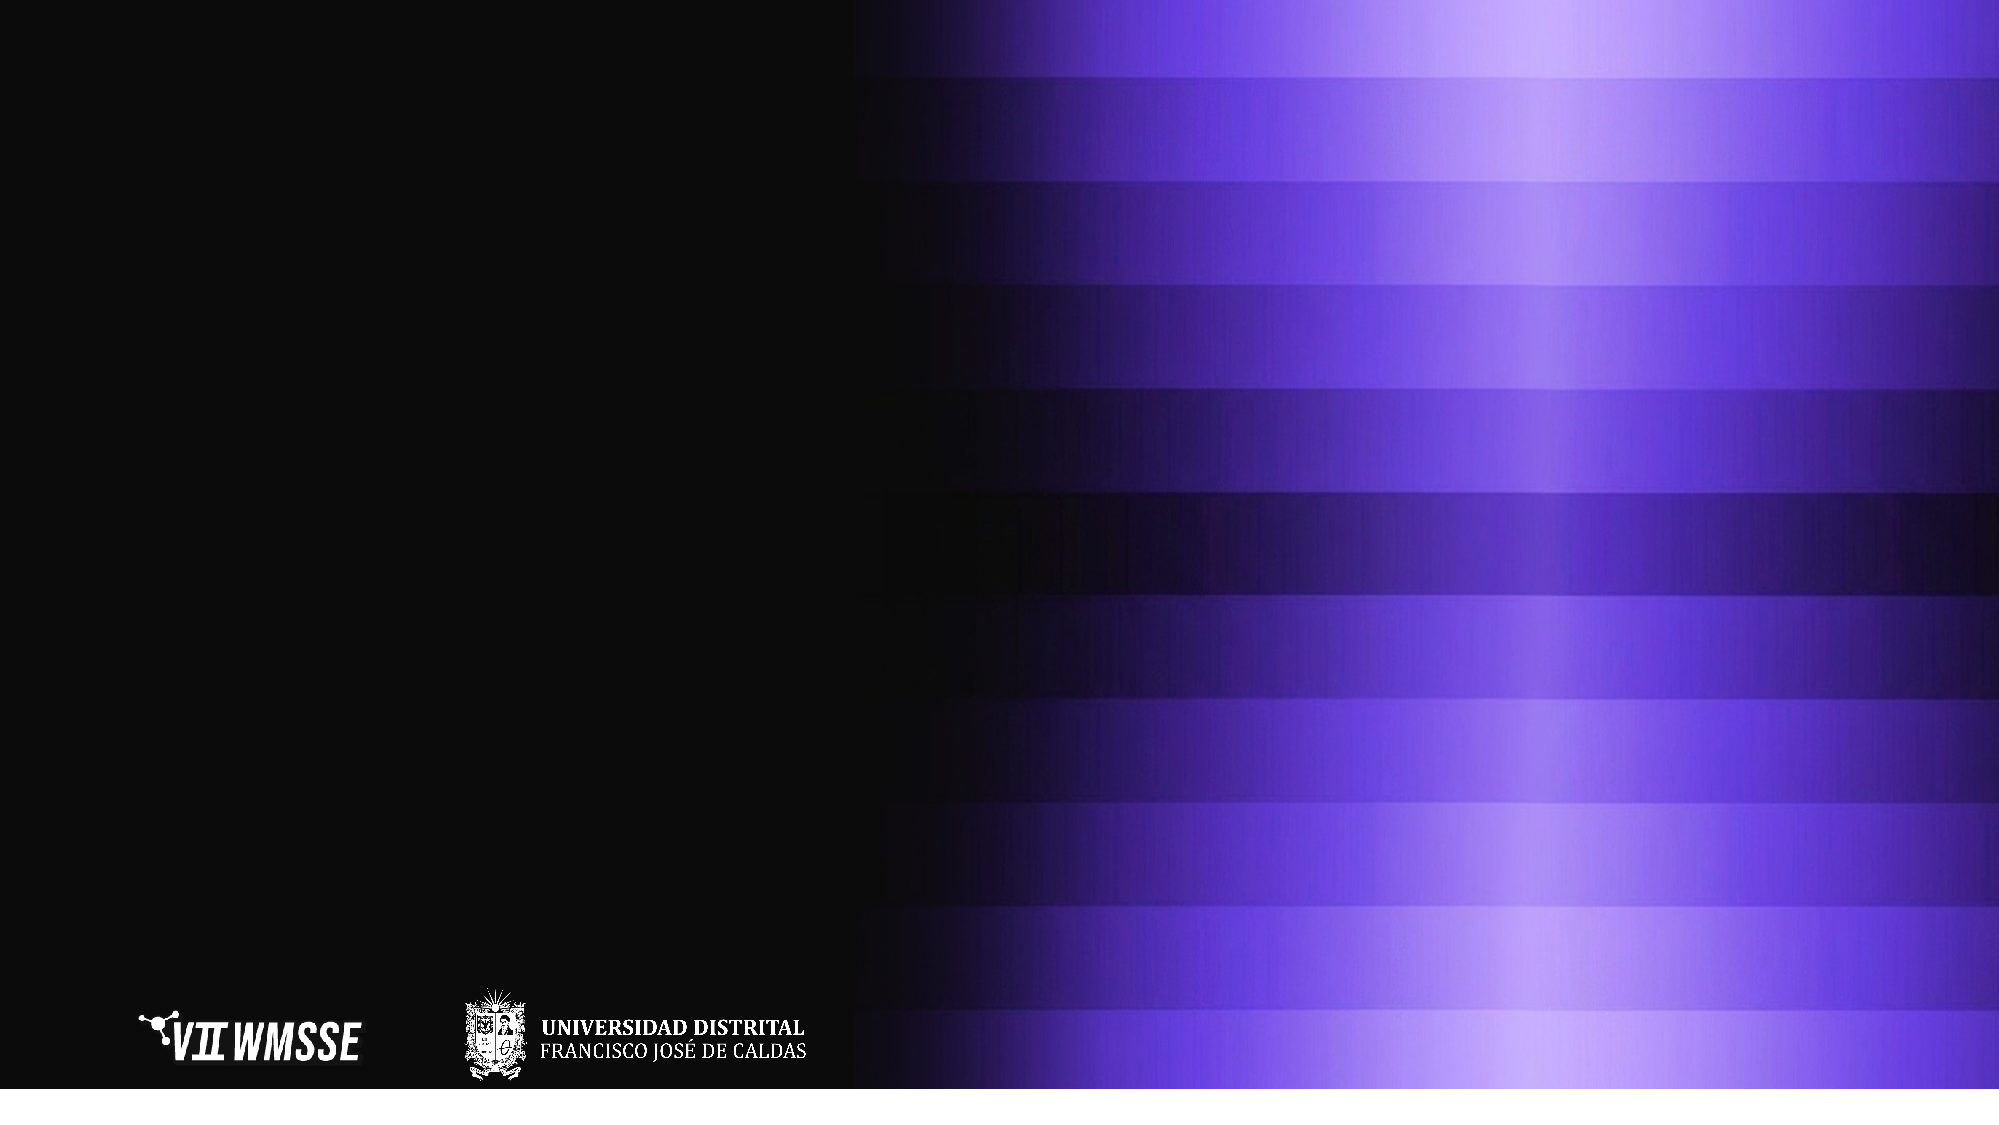
\includegraphics[width=\paperwidth,height=\paperheight]{Fondos/portada.pdf}}
  
  \setbeamercolor{title}{fg=backframe_color}
  \setbeamercolor{author}{fg=backframe_color}
  \setbeamercolor{institute}{fg=backframe_color}
  \setbeamercolor{date}{fg=backframe_color}

  \begin{frame}
      \titlepage
  \end{frame}
}

% ==========================================================
% Cuerpo: Letras Negras
% ==========================================================
{
  \usebackgroundtemplate{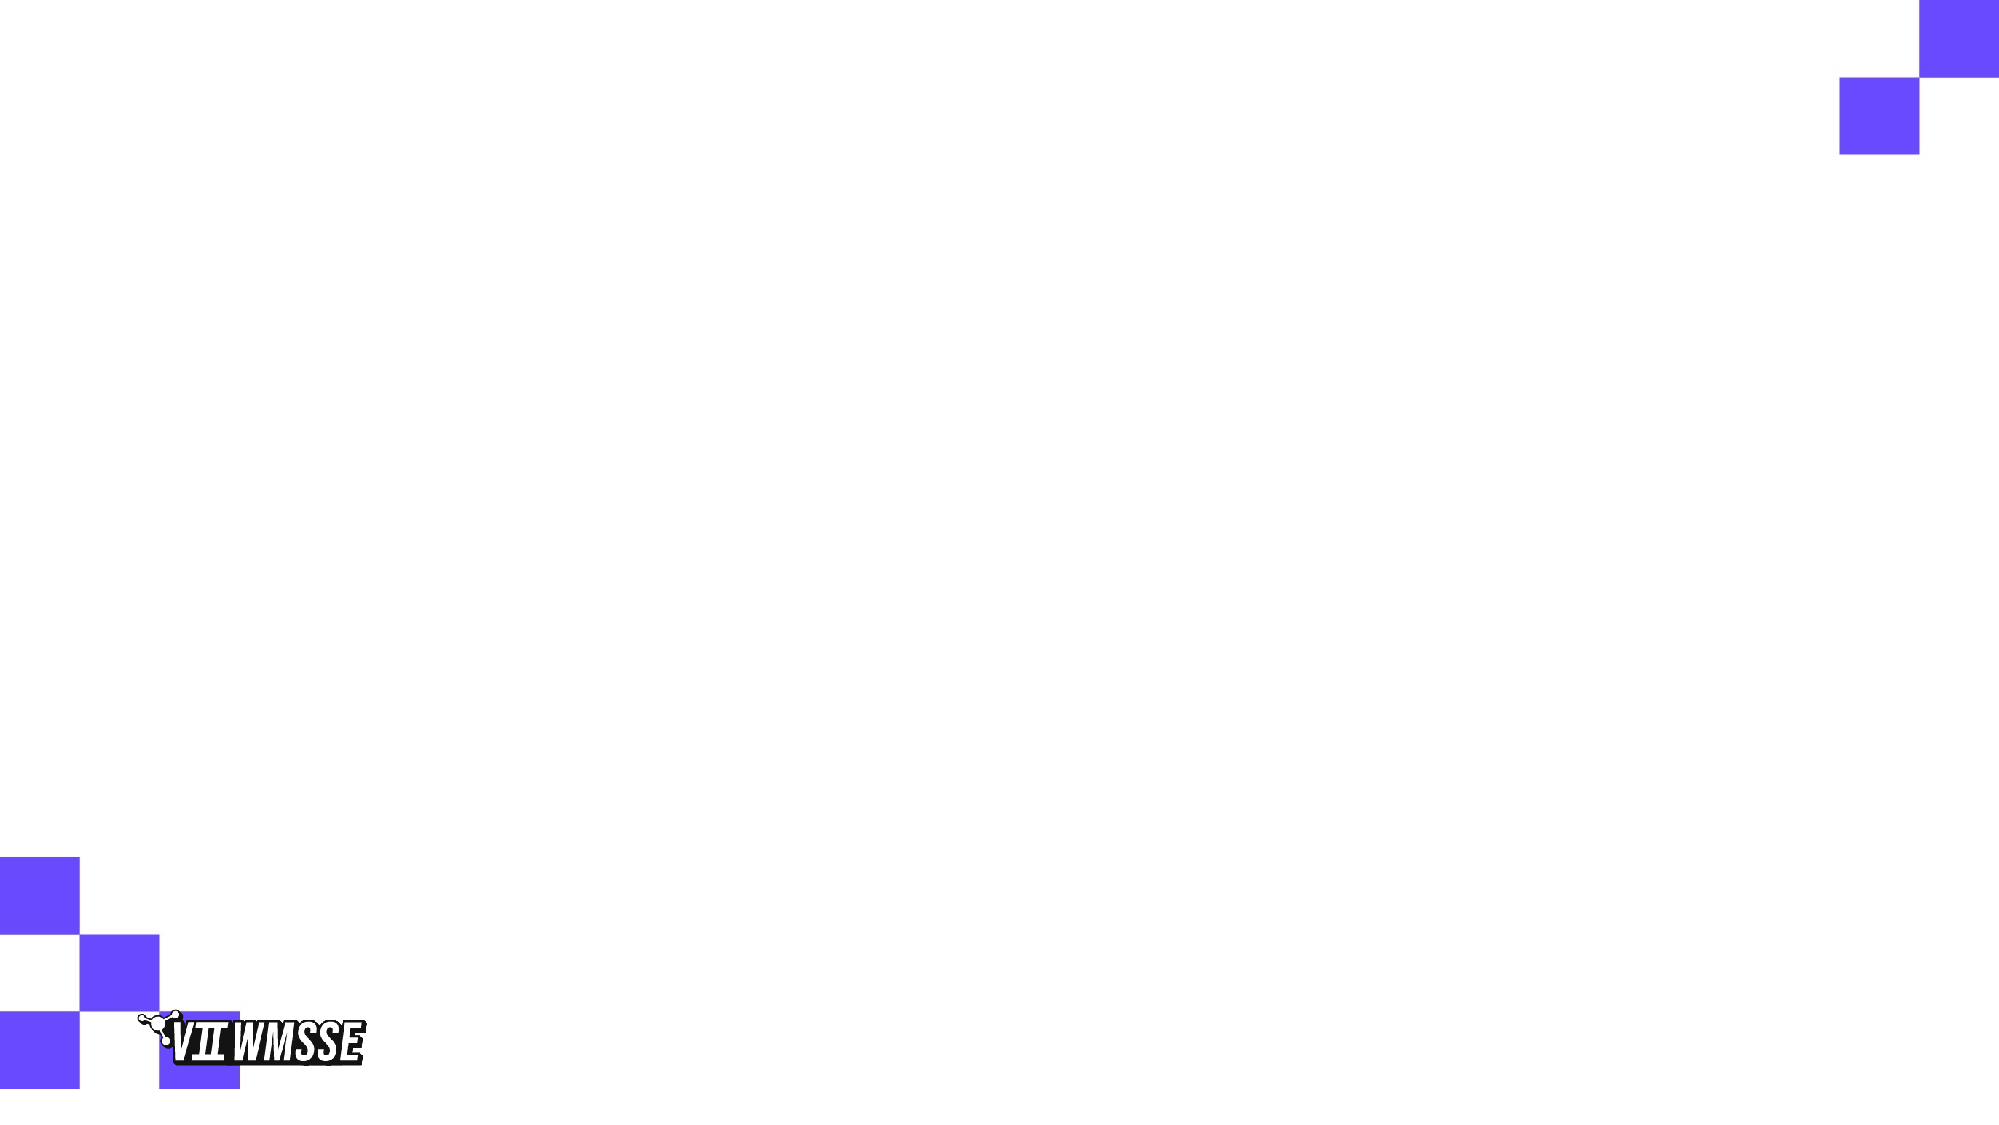
\includegraphics[width=\paperwidth,height=\paperheight]{Fondos/Cuerpo.pdf}hjzdbfkdfhaj}

  % Forzamos color negro
  \setbeamercolor{frametitle}{fg=white}
  \setbeamercolor{normal text}{fg=black}
  \setbeamercolor{structure}{fg=black}
  \setbeamercolor{itemize item}{fg=black}

%------------------------------------------------
% ÍNDICE
\begin{frame}{Contenido}
\tableofcontents
\end{frame}
}


%==========================================================
{
  \usebackgroundtemplate{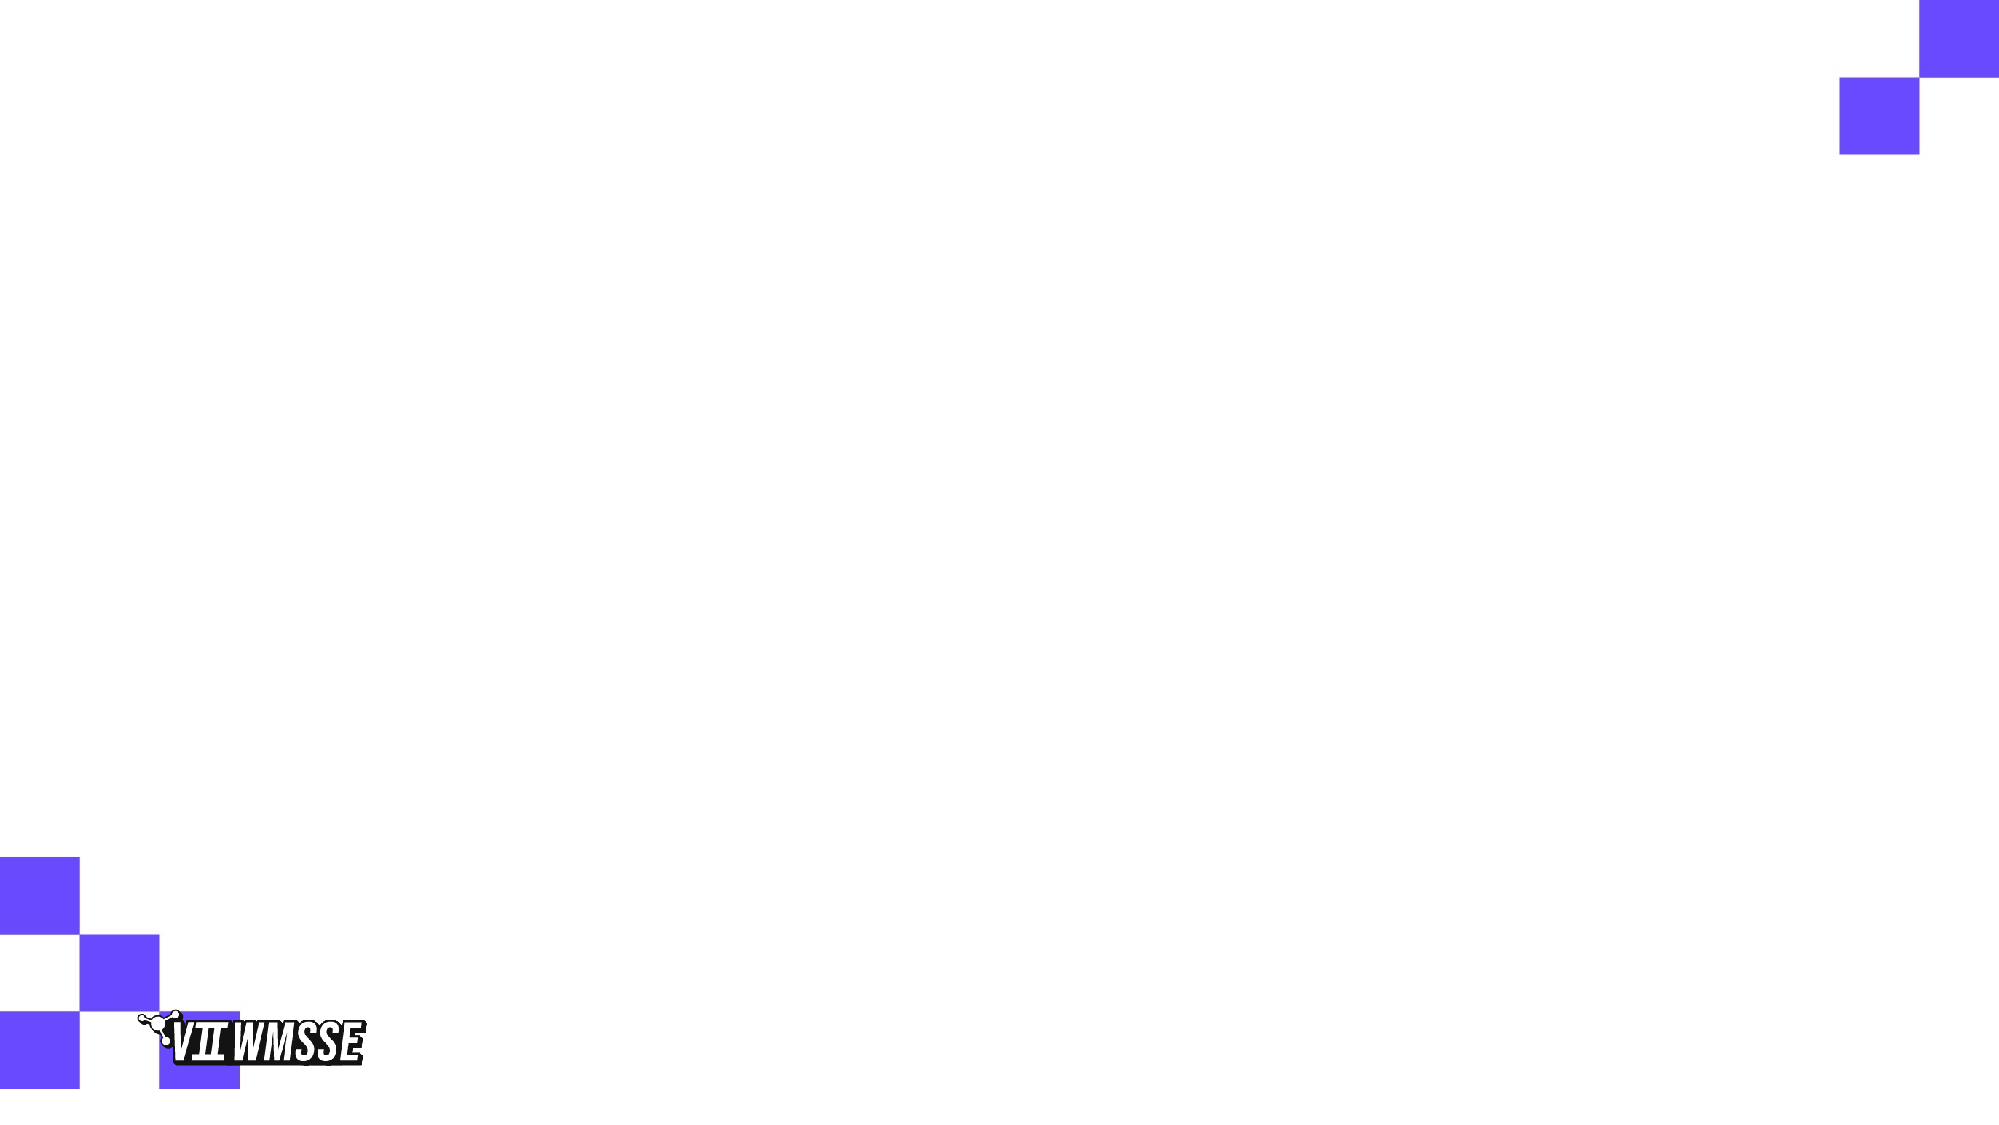
\includegraphics[width=\paperwidth,height=\paperheight]{Fondos/Cuerpo.pdf}}

  % Forzamos color negro
  \setbeamercolor{frametitle}{fg=white}
  \setbeamercolor{normal text}{fg=black}
  \setbeamercolor{structure}{fg=black}
  \setbeamercolor{itemize item}{fg=black}


\begin{frame}{Historia}

    \centering
    \begin{tikzpicture}[node distance=1cm, font=\small]

      % 1. Línea base horizontal (con el color de tu beamer)
      \draw[ultra thick, beamer_color, -latex] (-1,0) -- (14,0);

      % 2. HITOS (Círculos y Conectores)
      % Hito 1
      \filldraw[beamer_color] (1,0) circle (3pt);
      \draw[thick, gray, dashed] (1,0) -- (1,0.8);
      
      % Hito 2
      \filldraw[beamer_color] (3.5,0) circle (3pt);
      \draw[thick, gray, dashed] (3.5,0) -- (3.5,-0.8);
      
      % Hito 3
      \filldraw[beamer_color] (6,0) circle (3pt);
      \draw[thick, gray, dashed] (6,0) -- (6,0.8);
      
      % Hito 4
      \filldraw[beamer_color] (8.5,0) circle (3pt);
      \draw[thick, gray, dashed] (8.5,0) -- (8.5,-0.8);

      % Hito 5
      \filldraw[beamer_color] (11,0) circle (3pt);
      \draw[thick, gray, dashed] (11,0) -- (11,0.8);


      % 3. TEXTOS Y CAJAS (Alternados arriba y abajo para ganar espacio)
      
      % Año / Fase 1 (Arriba)
      \node[anchor=south, align=center] at (1, 0.8) {
        \textbf{\textcolor{beamer_color}{1911}} \\  
        \scriptsize Onnes licúa helio y descubre\\ \scriptsize que la resistividad del mercurio\\ \scriptsize colapsa a cero en T = 4.2 K.
      };

      % Año / Fase 2 (Abajo)
      \node[anchor=north, align=center] at (3.5, -0.8) {
        \textbf{\textcolor{beamer_color}{1933}}\\
        \scriptsize Meissner y Ochsenfeld descubren\\
        \scriptsize la expulsión perfecta del campo\\
        \scriptsize  magnético la superconductividad no es\\
        \scriptsize solo conductividad perfecta.
      };

      % Año / Fase 3 (Arriba)
      \node[anchor=south, align=center] at (6, 0.8) {
        \textbf{\textcolor{beamer_color}{1950}} \\ 
        \scriptsize Ginzburg y Landau proponen\\
        \scriptsize a teoría fenomenológica\\
        \scriptsize con parámetro de orden complejo $\psi$.
      };

      % Año / Fase 4 (Abajo)
      \node[anchor=north, align=center] at (8.5, -0.8) {
        \textbf{\textcolor{beamer_color}{1957}} \\ 
        \scriptsize Bardeen, Cooper y Schrieffer \\
        \scriptsize explican microscópicamente el\\
        \scriptsize mecanismo: pares de Cooper\\
        \scriptsize mediados por fonones, brecha\\
        \scriptsize de energía $\Delta$.
      };

      % Año / Fase 5 (Arriba)
      \node[anchor=south, align=center] at (11, 0.8) {
        \textbf{\textcolor{beamer_color}{1962}} \\ 
        \scriptsize Josephson predice el efecto\\
        \scriptsize túnel de pares de Cooper\\
        \scriptsize entre dos superconductores\\
        \scriptsize separados por una barrera delgada.
      };

    \end{tikzpicture}

  \end{frame}
}

%==========================================================
{
  \usebackgroundtemplate{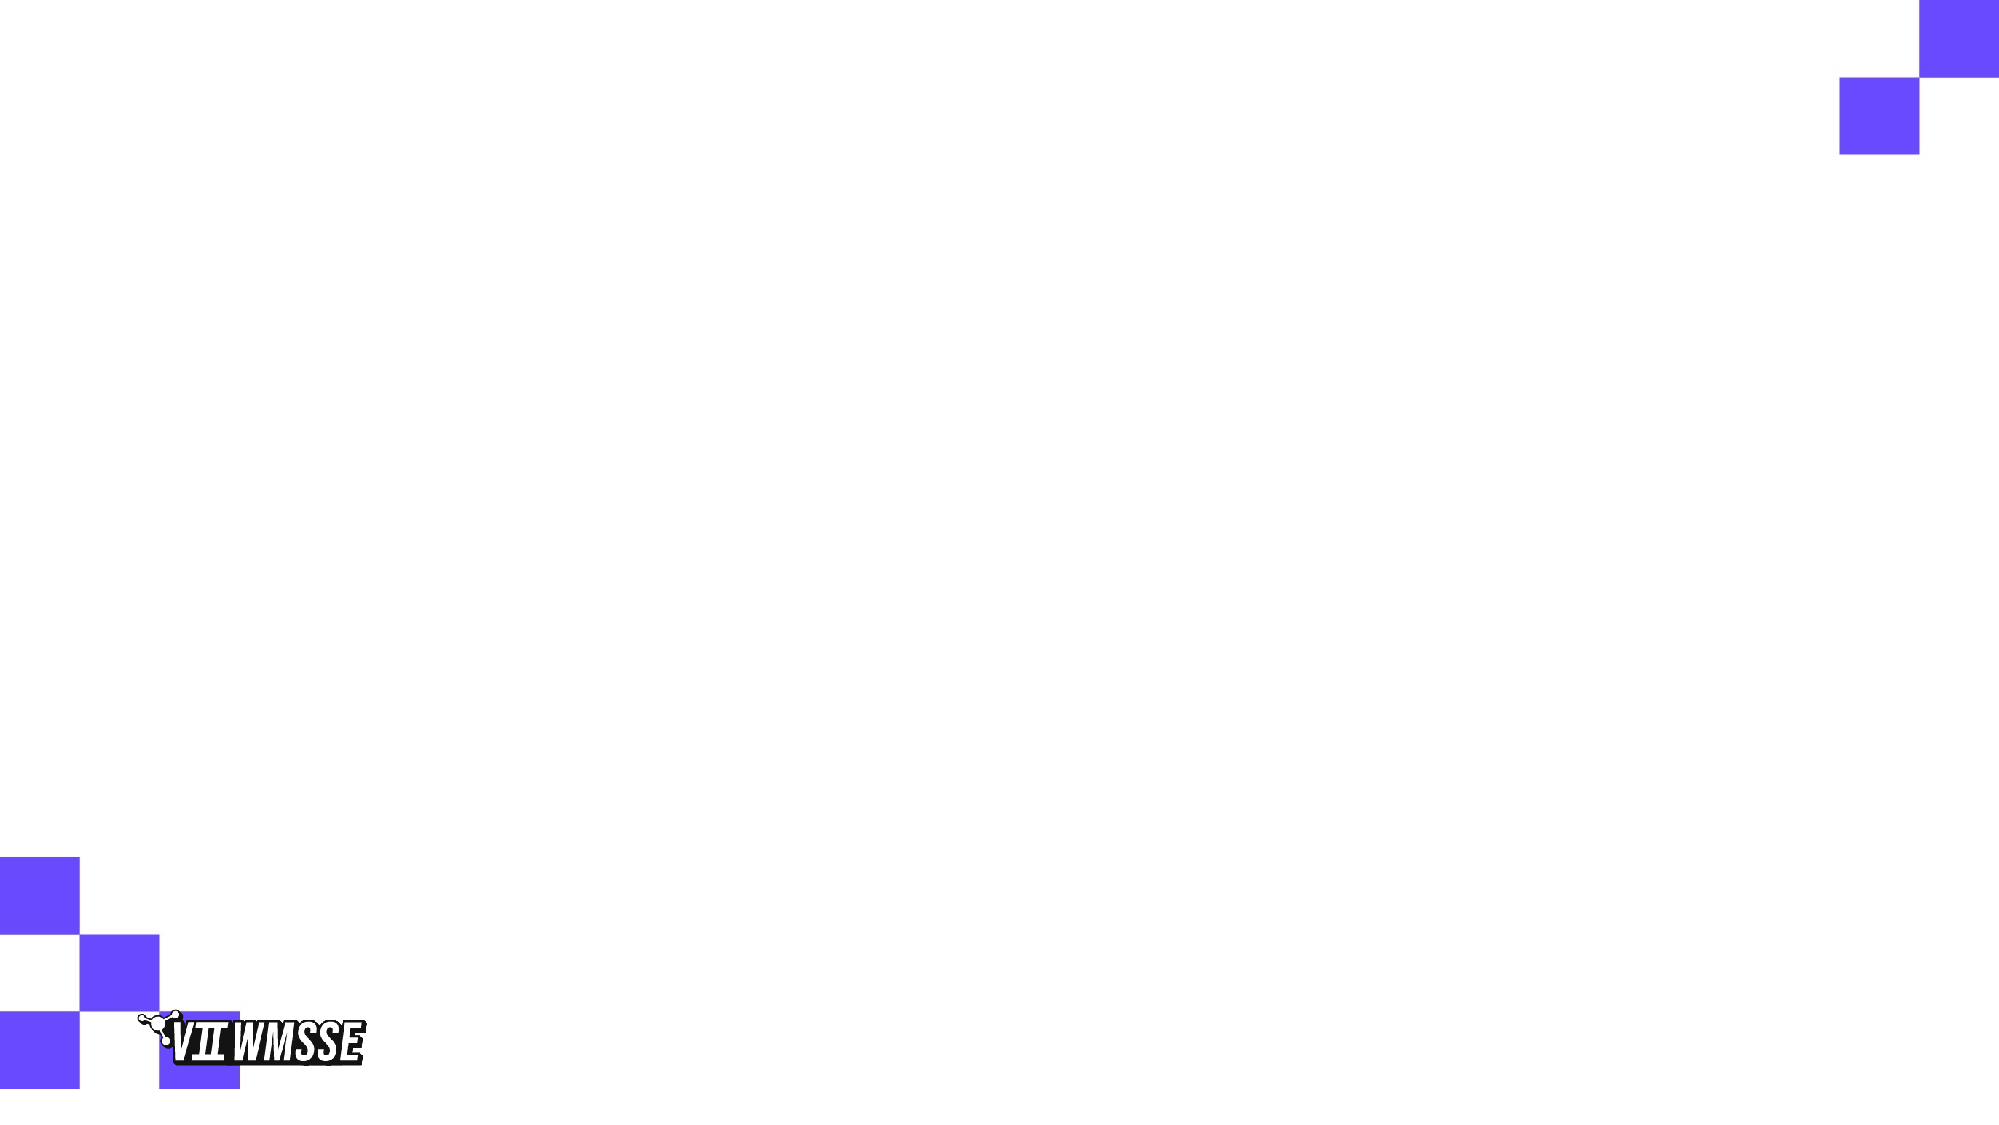
\includegraphics[width=\paperwidth,height=\paperheight]{Fondos/Cuerpo.pdf}}

  % Forzamos color negro
  \setbeamercolor{frametitle}{fg=white}
  \setbeamercolor{normal text}{fg=black}
  \setbeamercolor{structure}{fg=black}
  \setbeamercolor{itemize item}{fg=black}


\begin{frame}{Historia}

    \centering
    \begin{tikzpicture}[node distance=1cm, font=\small]

      % 2. HITOS (Círculos y Conectores)
      % 1. Línea base horizontal (con el color de tu beamer)
      \draw[ultra thick, beamer_color, -latex] (0,0) -- (13,0);

      % 2. HITOS (Círculos y Conectores)
      % Hito 1
      \filldraw[beamer_color] (1.5,0) circle (3pt);
      \draw[thick, gray, dashed] (1.5,0) -- (1.5,0.8);
      
      % Hito 2
      \filldraw[beamer_color] (4.5,0) circle (3pt);
      \draw[thick, gray, dashed] (4.5,0) -- (4.5,-0.8);
      
      % Hito 3
      \filldraw[beamer_color] (7.5,0) circle (3pt);
      \draw[thick, gray, dashed] (7.5,0) -- (7.5,0.8);
      
      % Hito 4
      \filldraw[beamer_color] (10.5,0) circle (3pt);
      \draw[thick, gray, dashed] (10.5,0) -- (10.5,-0.8);


      % 3. TEXTOS Y CAJAS (Alternados arriba y abajo para ganar espacio)
      
      % Año / Fase 1 (Arriba)
      \node[anchor=south, align=center] at (1.5, 0.8) {
        \textbf{\textcolor{beamer_color}{1986-1987}} \\  
        \scriptsize Bednorz y Müller descubren \\ 
        \scriptsize $La_2CuO_4$ con $Tc \approx 35$ K, catalizando\\
        \scriptsize la búsqueda de cupratos de alta Tc.
      };

      % Año / Fase 2 (Abajo)
      \node[anchor=north, align=center] at (4.5, -0.8) {
        \textbf{\textcolor{beamer_color}{2001}}\\
        \scriptsize Descubrimiento de $MgB_2$\\
        \scriptsize superconductor convencional \\
        \scriptsize  con Tc sorprendentemente alta.
      };

      % Año / Fase 3 (Arriba)
      \node[anchor=south, align=center] at (7.5, 0.8) {
        \textbf{\textcolor{beamer_color}{2008}} \\ 
        \scriptsize Superconductores de pnicturo\\
        \scriptsize de hierro (familia LaFeAsO).
      };

      % Año / Fase 4 (Abajo)
      \node[anchor=north, align=center] at (10.5, -0.8) {
        \textbf{\textcolor{beamer_color}{Actualidad}} \\ 
        \scriptsize Nanoarquitecturas mesoscópicas 3D, \\
        \scriptsize control de vórtices individual,\\
        \scriptsize electrónica superconductora de\\
        \scriptsize ultra-bajo consumo.
      };

    \end{tikzpicture}

  \end{frame}
}

%====================================1===============
{
  \usebackgroundtemplate{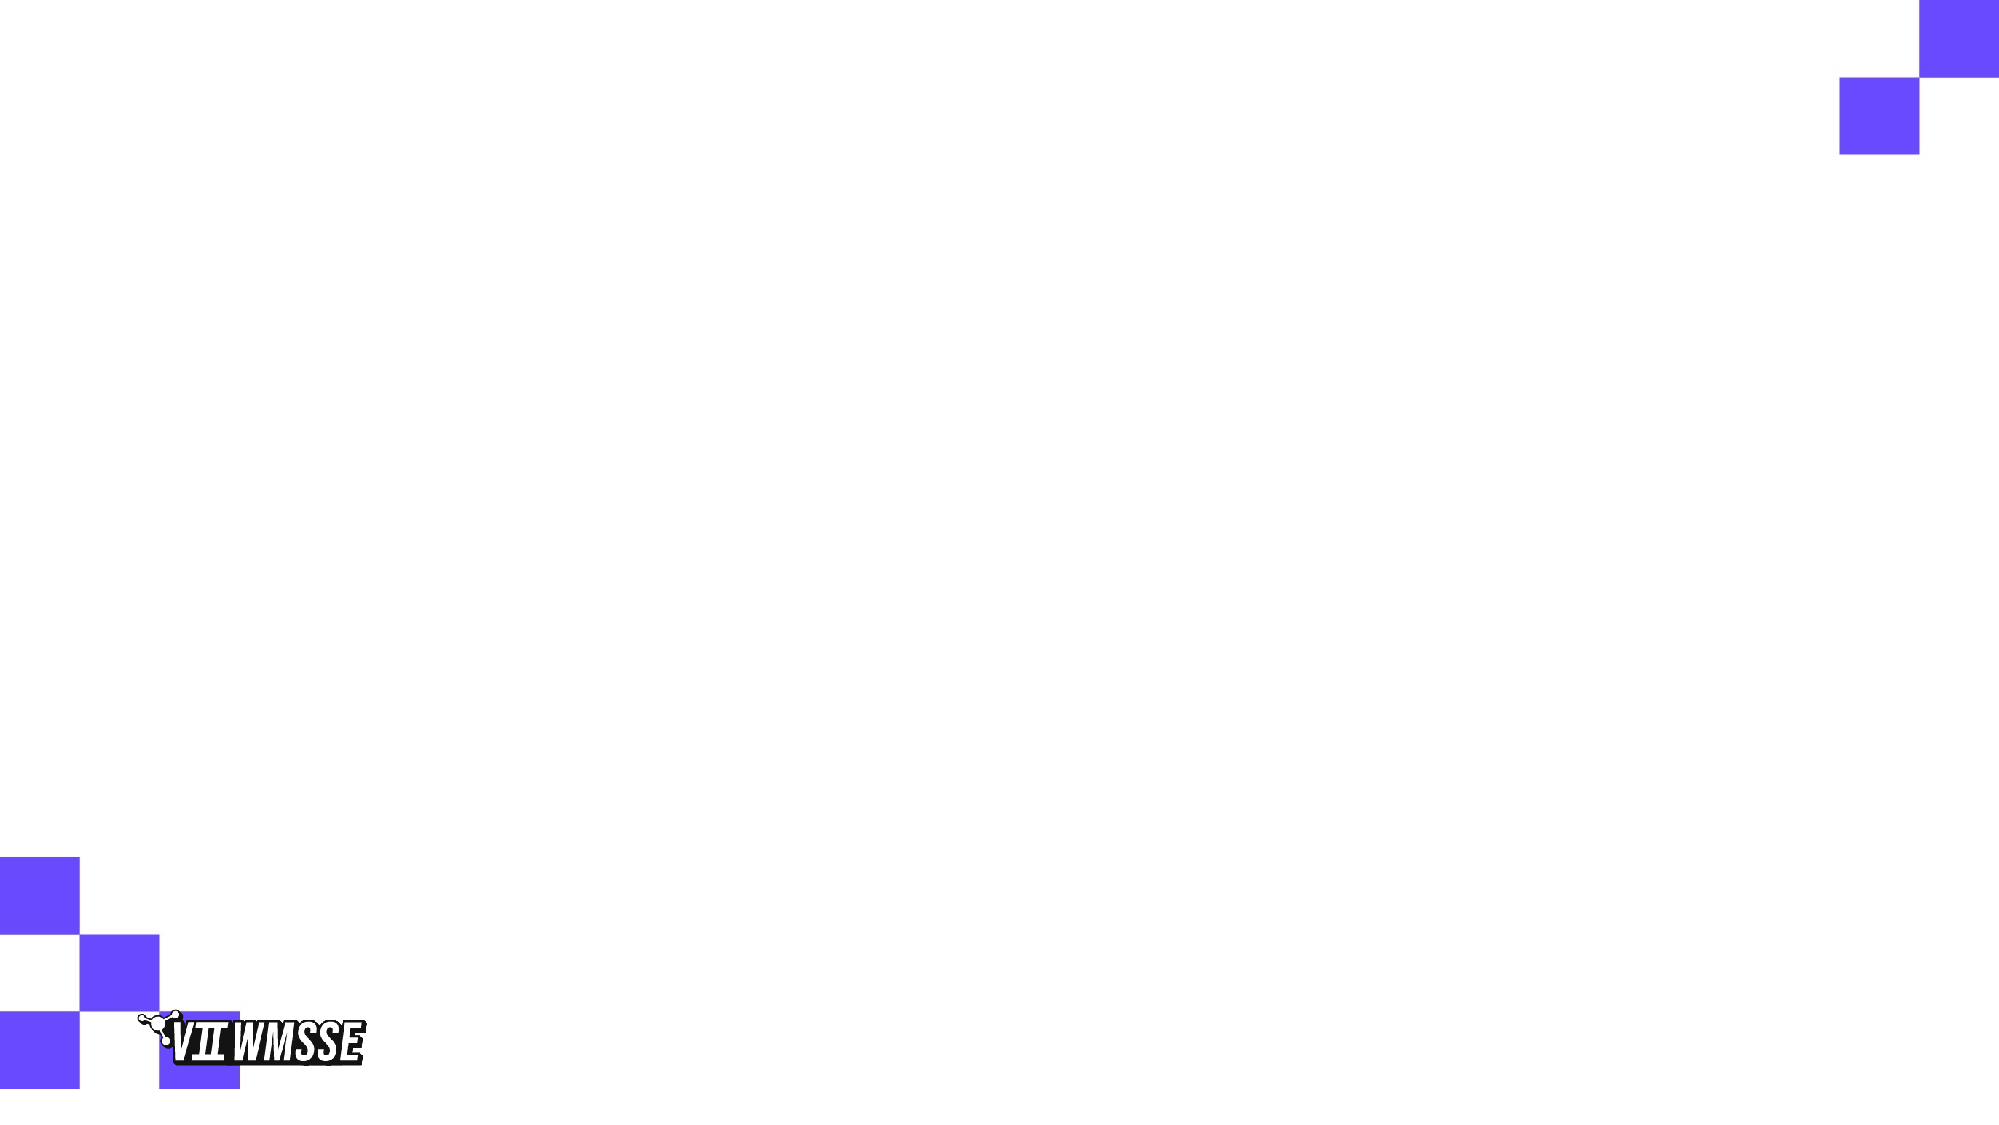
\includegraphics[width=\paperwidth,height=\paperheight]{Fondos/Cuerpo.pdf}}

  % Forzamos color negro
  \setbeamercolor{frametitle}{fg=white}
  \setbeamercolor{normal text}{fg=black}
  \setbeamercolor{structure}{fg=black}
  \setbeamercolor{itemize item}{fg=black}

  

\section{Historia y Premios Nobel de la Superconductividad}
\begin{frame}{Premios Nobel de la Superconductividad}

    \centering
    \begin{tikzpicture}[node distance=1cm, font=\small]

      % 1. Línea base horizontal (con el color de tu beamer)
      \draw[ultra thick, beamer_color, -latex] (0,0) -- (13,0);

      % 2. HITOS (Círculos y Conectores)
      % Hito 1
      \filldraw[beamer_color] (1.5,0) circle (3pt);
      \draw[thick, gray, dashed] (1.5,0) -- (1.5,0.8);
      
      % Hito 2
      \filldraw[beamer_color] (4.5,0) circle (3pt);
      \draw[thick, gray, dashed] (4.5,0) -- (4.5,-0.8);
      
      % Hito 3
      \filldraw[beamer_color] (7.5,0) circle (3pt);
      \draw[thick, gray, dashed] (7.5,0) -- (7.5,0.8);
      
      % Hito 4
      \filldraw[beamer_color] (10.5,0) circle (3pt);
      \draw[thick, gray, dashed] (10.5,0) -- (10.5,-0.8);


      % 3. TEXTOS Y CAJAS (Alternados arriba y abajo para ganar espacio)
      
      % Año / Fase 1 (Arriba)
      \node[anchor=south, align=center] at (1.5, 0.8) {
        \textbf{\textcolor{beamer_color}{1913}} \\ 
        \textbf{Heike Kamerlingh Onnes} \\ 
        \scriptsize Licuefacción del helio\\ \scriptsize y descubrimiento de la\\ \scriptsize superconductividad en Hg a 4.2 K
      };

      % Año / Fase 2 (Abajo)
      \node[anchor=north, align=center] at (4.5, -0.8) {
        \textbf{\textcolor{beamer_color}{1972}} \\ 
        \textbf{John Bardeen, Leon Cooper,}\\ \textbf{John R. Schrieffer} \\ 
        \scriptsize Teoría BCS microscópica\\ \scriptsize de la superconductividad
      };

      % Año / Fase 3 (Arriba)
      \node[anchor=south, align=center] at (7.5, 0.8) {
        \textbf{\textcolor{beamer_color}{1987}} \\ 
        \textbf{Georg Bednorz, K. Alex Müller} \\ 
        \scriptsize Contribuciones a la teoría de superconductores y\\ \scriptsize Descubrimiento de superconductividad\\ \scriptsize de alta temperatura en cupratos
      };

      % Año / Fase 4 (Abajo)
      \node[anchor=north, align=center] at (10.5, -0.8) {
        \textbf{\textcolor{beamer_color}{2003}} \\ 
        \textbf{Alexei Abrikosov, Vitaly Ginzburg,}\\ \textbf{Anthony Leggett} \\ 
        \scriptsize Contribuciones a la teoría de superconductores y\\ \scriptsize superfluidos (vórtices de\\ \scriptsize Abrikosov, teoría GL)
      };

    \end{tikzpicture}

  \end{frame}
}

%============================2=======================
{
  \usebackgroundtemplate{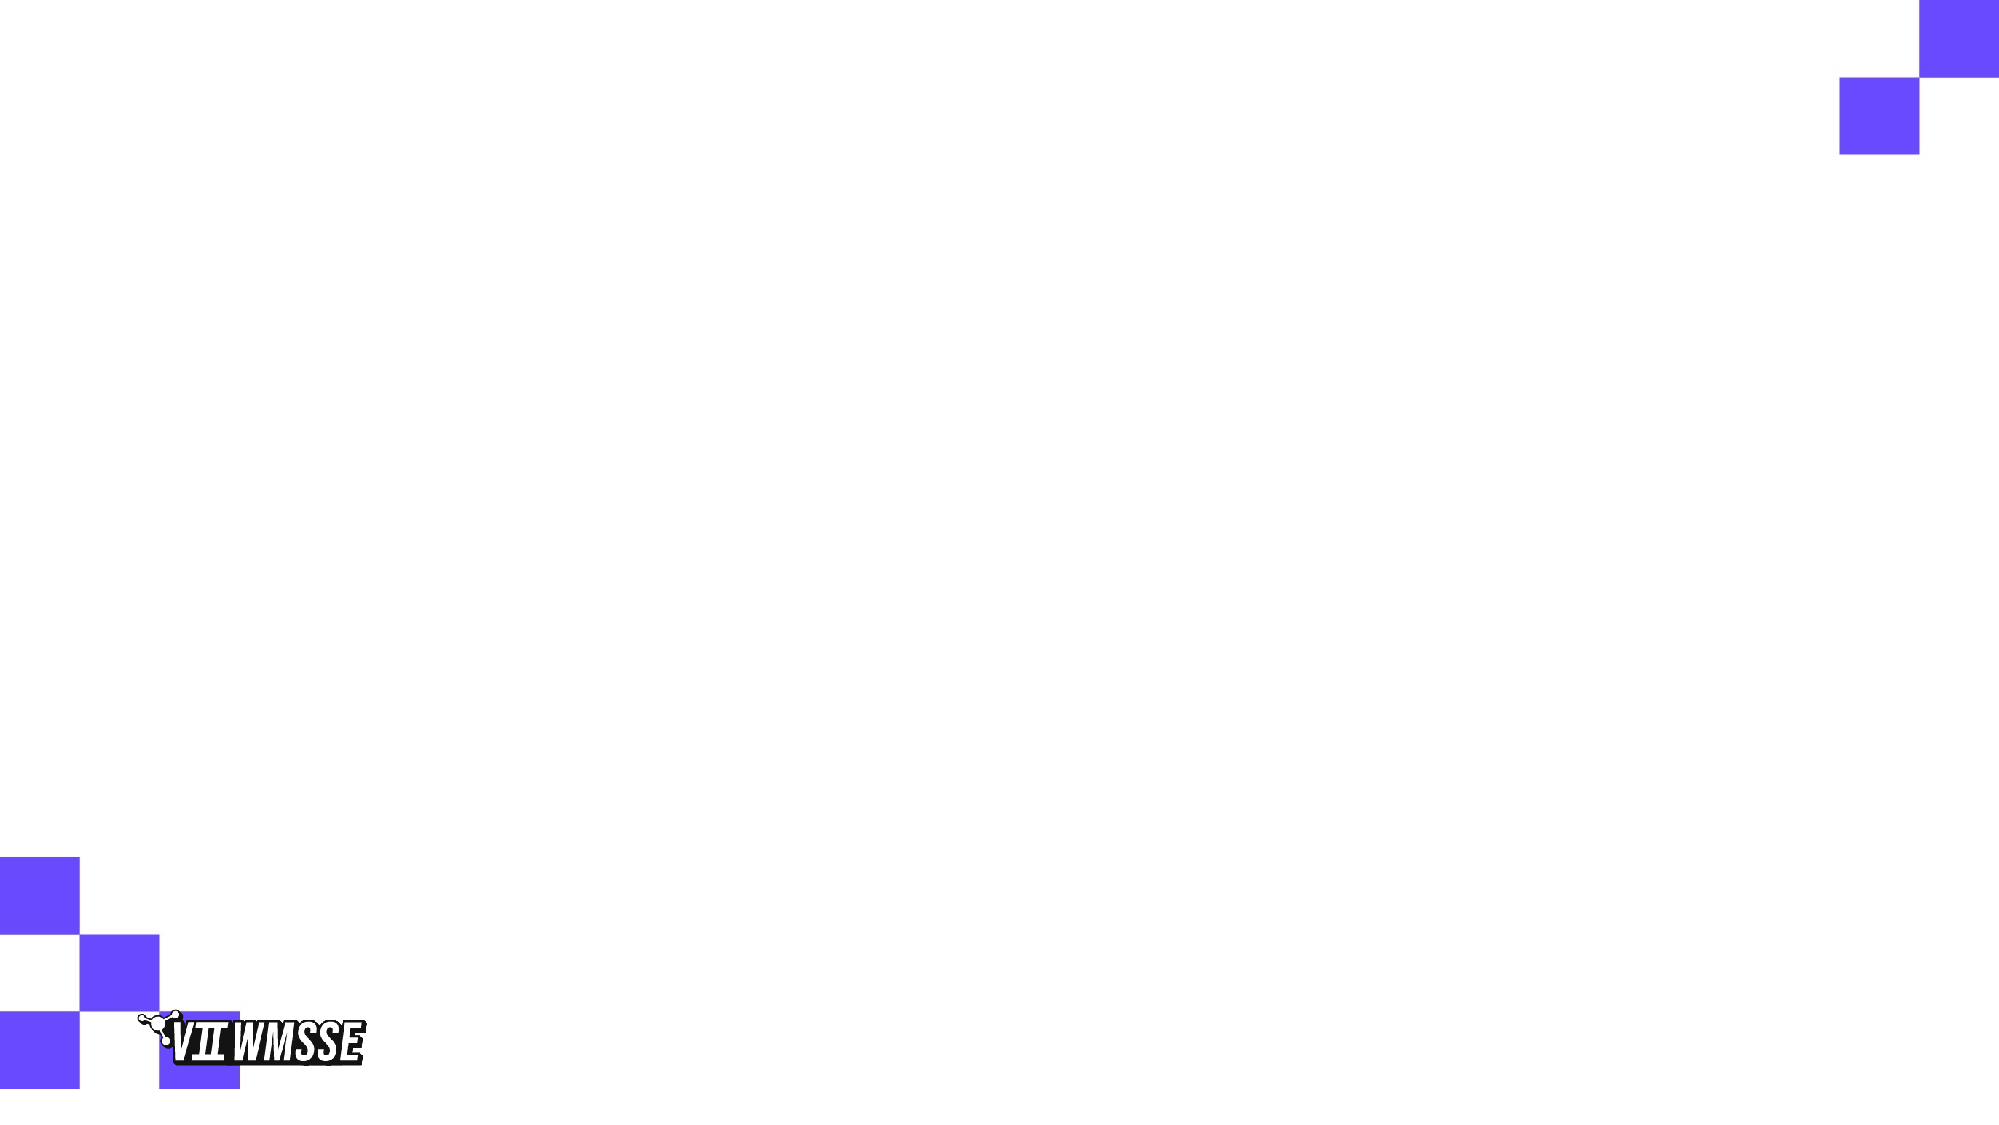
\includegraphics[width=\paperwidth,height=\paperheight]{Fondos/Cuerpo.pdf}}

  % Forzamos color negro
  \setbeamercolor{frametitle}{fg=white}
  \setbeamercolor{normal text}{fg=black}
  \setbeamercolor{structure}{fg=black}
  \setbeamercolor{itemize item}{fg=black}

\section{Marco Teórico y Formalismo Matemático}
  \begin{frame}{Bardeen, Cooper y Schrieffer (1957)}
    \framesubtitle{Subtítulo aquí}

    \begin{columns}[c]

        % Columna izquierda
        \begin{column}{0.58\textwidth}

            \begin{itemize}
                \item Electrones que se atraen debido a la interacción mediada por fonones.
                \item La atracción solo funciona para electrones cuya energía está dentro de una 'cáscara delgada' alrededor del nivel de Fermi.
                \item La atracción solo puede actuar sobre electrones en la superficie de Fermi, donde hay estados disponibles.
                \item Basta con una atracción débil para producir un par de Cooper.
            \end{itemize}

        \end{column}

        % Columna derecha
        \begin{column}{0.38\textwidth}

            \centering
            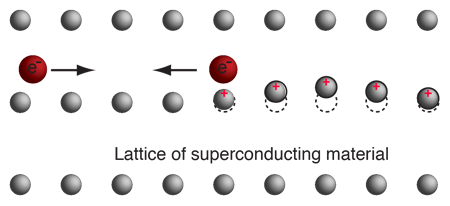
\includegraphics[width=1\linewidth]{Imagenes/BCS}

        \end{column}

    \end{columns}

\end{frame}
}

%=================================================
{
  \usebackgroundtemplate{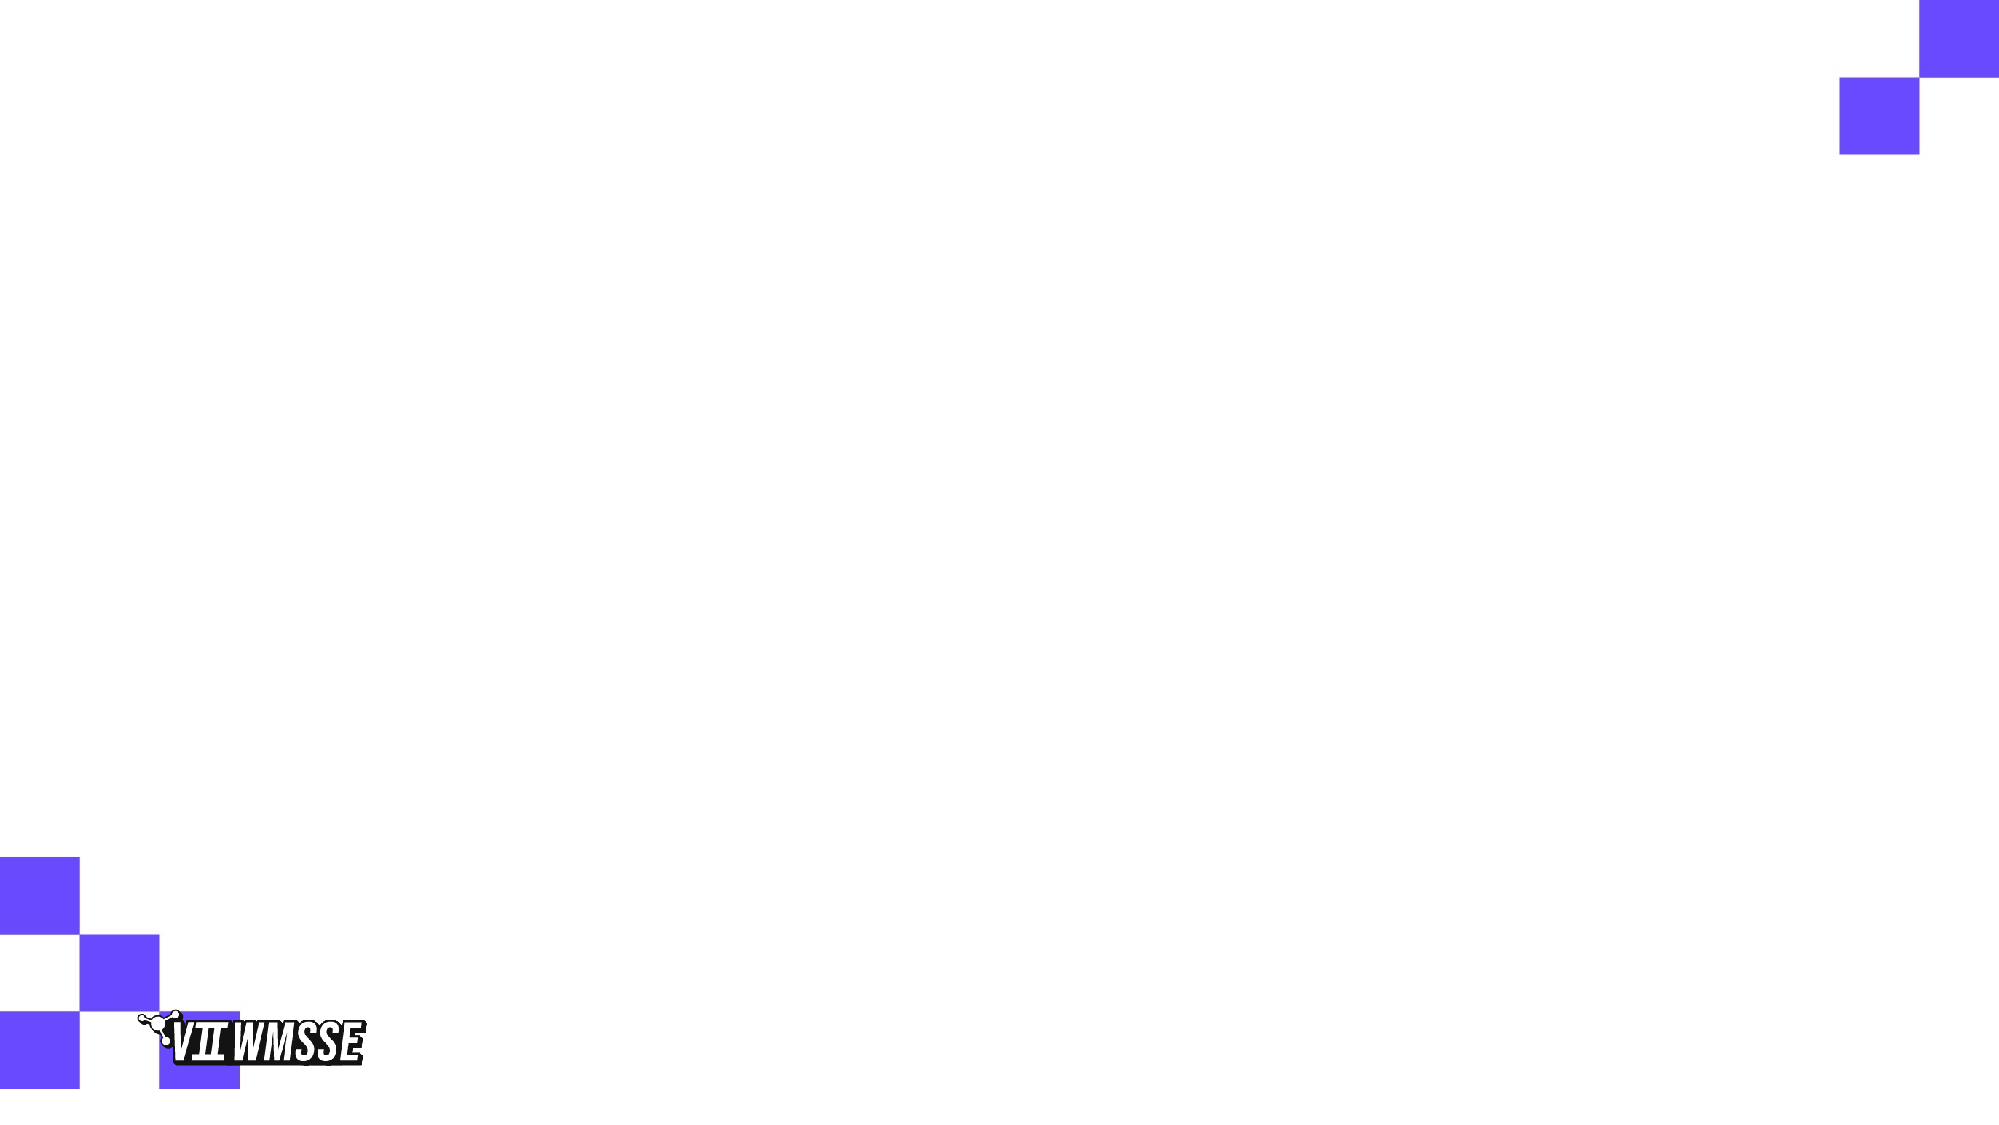
\includegraphics[width=\paperwidth,height=\paperheight]{Fondos/Cuerpo.pdf}}
  \setbeamercolor{frametitle}{fg=white}
  \setbeamercolor{normal text}{fg=black}
  \setbeamercolor{structure}{fg=black}
  \setbeamercolor{itemize item}{fg=black}

  \begin{frame}{BCS vs GL}
    \scriptsize 

    \begin{columns}[t]
      \begin{column}{0.48\textwidth}
        \begin{block}{\centering BCS}
          \centering
            \begin{itemize}
                \item Está formulada en el espacio de momentos
                \item Asume materiales homogéneos e infinitos
                \item Es realmente difícil tratar geometrías complejas, bordes, defectos o campos no uniformes
            \end{itemize}
        \end{block}
      \end{column}

      \begin{column}{0.48\textwidth}
        \begin{block}{\centering GL}
          \centering
            \begin{itemize}
                \item Ignora los electrones individuales
                \item Describe el estado superconductor con una sola función de onda macroscópica
                \item Se puede tratar cualquier geometría, cualquier inhomogeneidad, y cualquier distribución de campo
            \end{itemize}
        \end{block}
      \end{column}
    \end{columns}
  \end{frame}
}

%=========================3==========================
{
  \usebackgroundtemplate{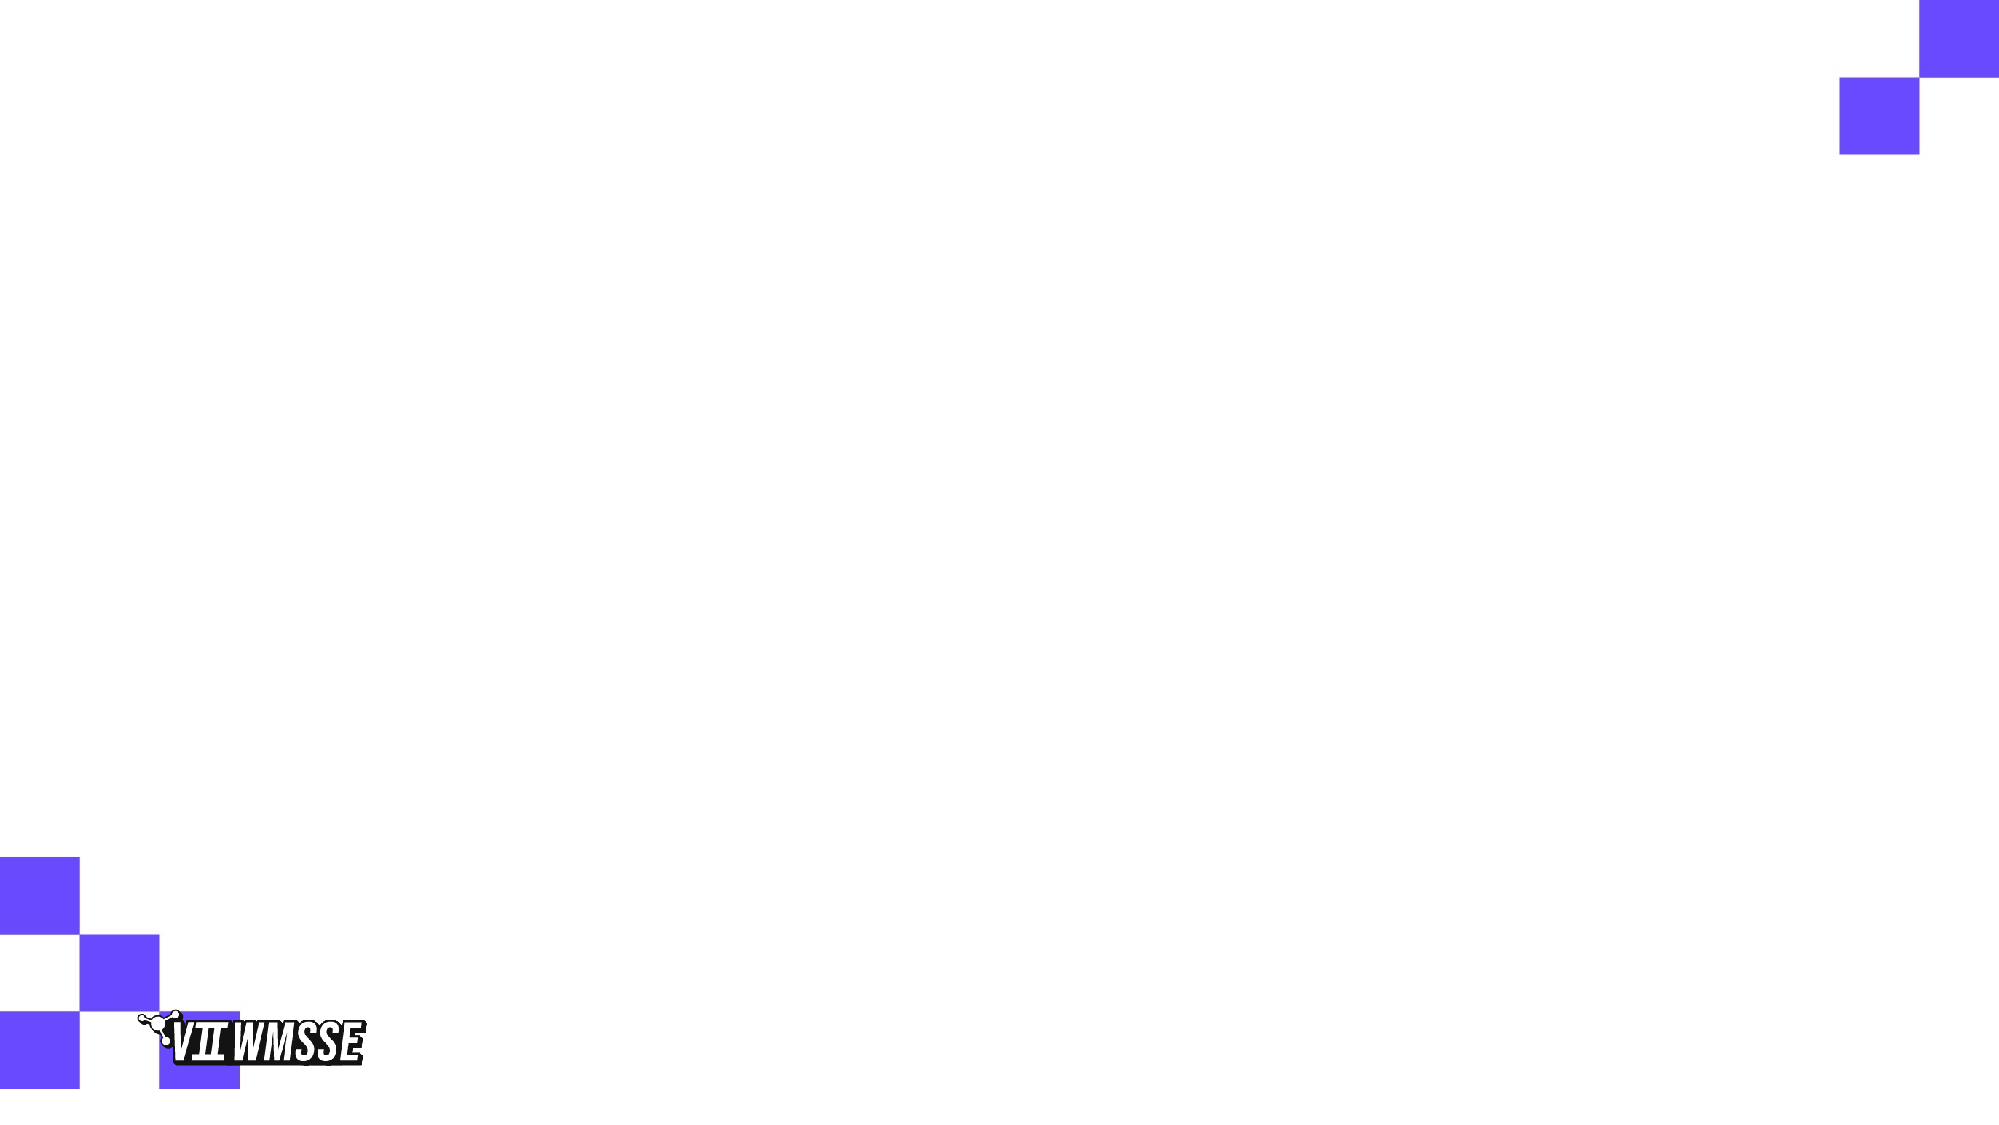
\includegraphics[width=\paperwidth,height=\paperheight]{Fondos/Cuerpo.pdf}}

  % Forzamos color negro
  \setbeamercolor{frametitle}{fg=white}
  \setbeamercolor{normal text}{fg=black}
  \setbeamercolor{structure}{fg=black}
  \setbeamercolor{itemize item}{fg=black}


  \begin{frame}{Teoría de Ginzburg-Landau (1950)}
  

    \begin{itemize}
        \item Landau propuso que toda transición de fase de segundo orden puede describirse introduciendo un parámetro de fase de orden que es 0 en la fase de alta simetría y distinto de 0 en la fase de baja simetría.
    
        \item Ginzburg y Landau propusieron que en un superconductor el parámetro de orden debe ser complejo:
        \begin{equation*}
            \psi (r) = \lvert \psi (r) \rvert e^{i\theta(r)}
        \end{equation*}

        
        \item La amplitud $\lvert \psi\rvert²$ mide la densidad local de pares de Cooper. La fase $\theta(r)$ contiene toda la información sobre el flujo de supercorriente y la coherencia cuántica.
    \end{itemize}

        
        
  \end{frame}
}


%=========================4==========================
{
  \usebackgroundtemplate{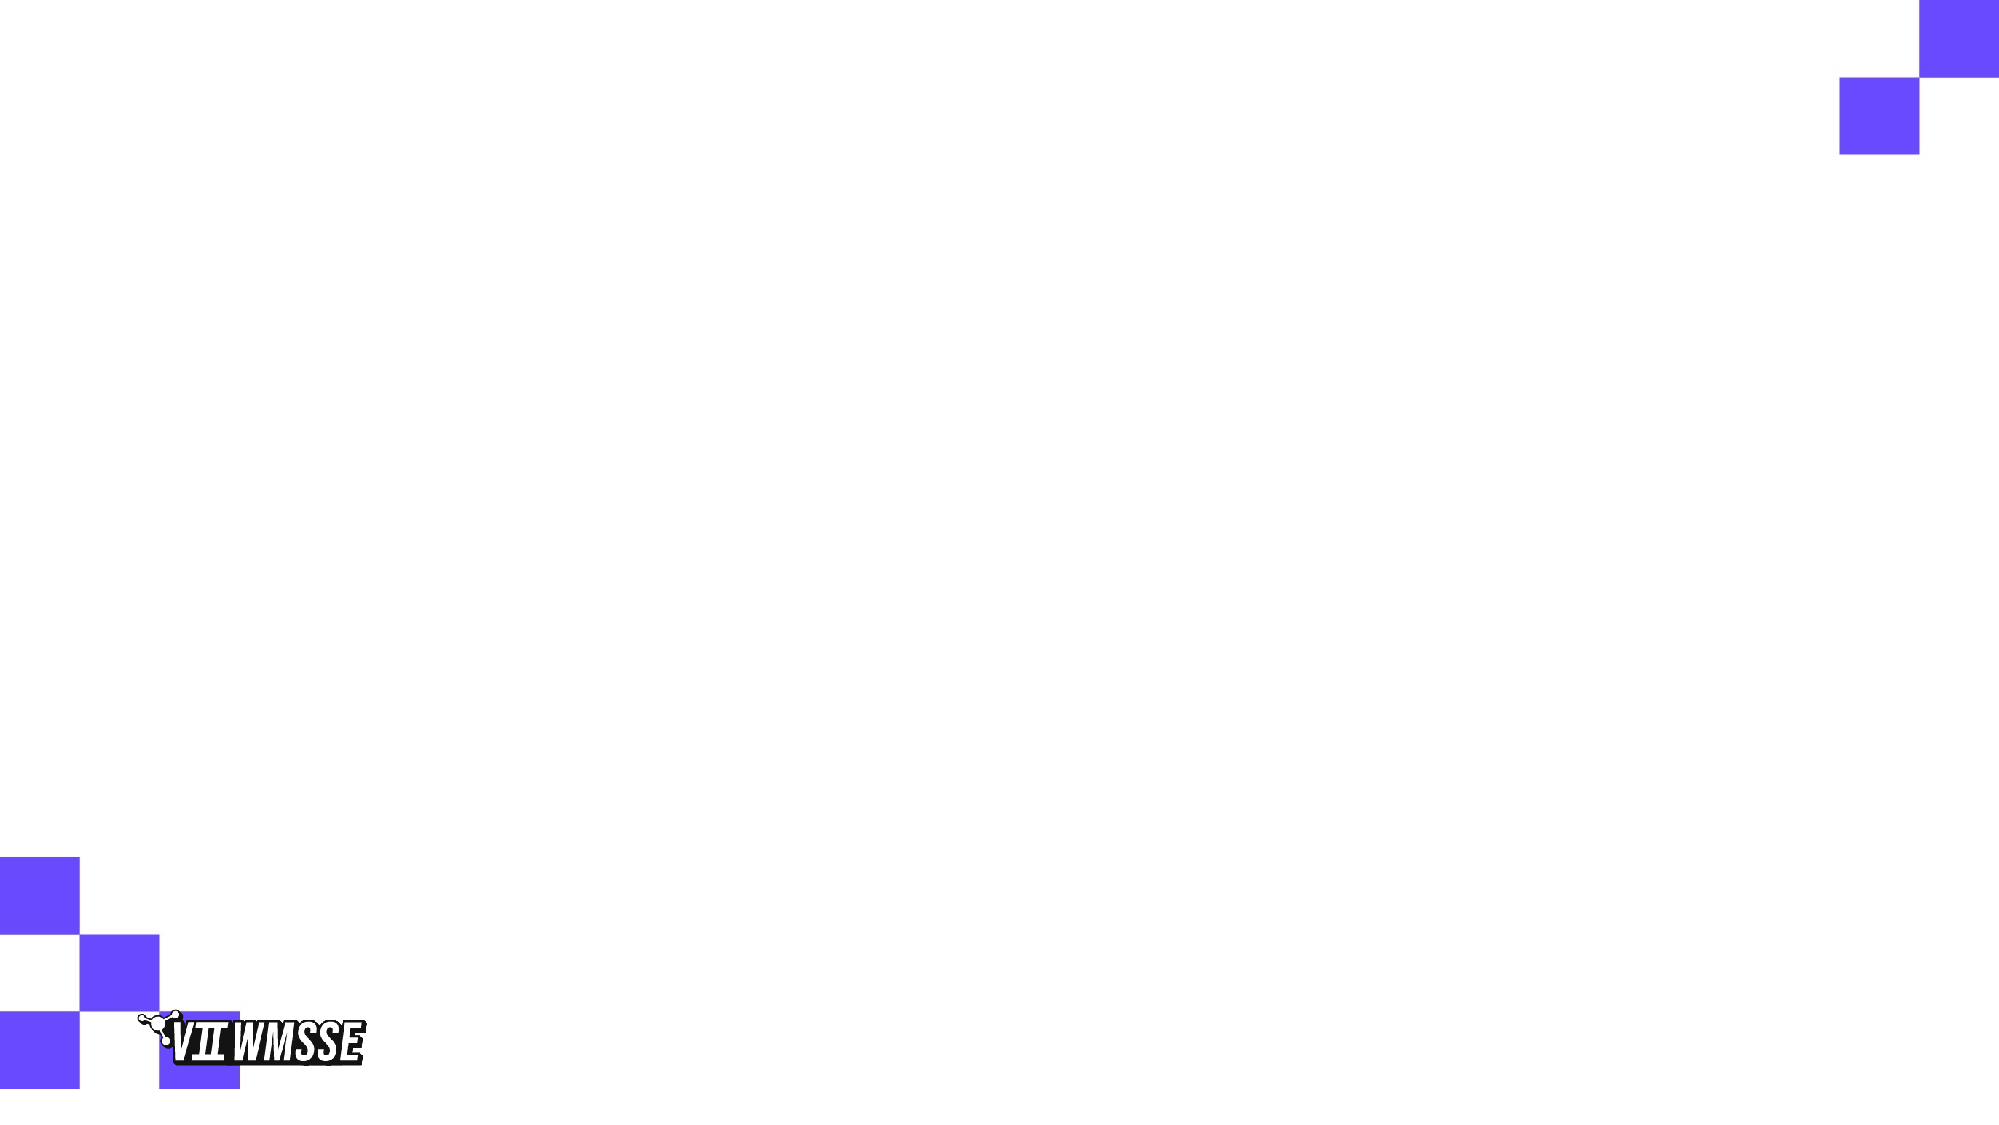
\includegraphics[width=\paperwidth,height=\paperheight]{Fondos/Cuerpo.pdf}}

  % Forzamos color negro
  \setbeamercolor{frametitle}{fg=white}
  \setbeamercolor{normal text}{fg=black}
  \setbeamercolor{structure}{fg=black}
  \setbeamercolor{itemize item}{fg=black}


  \begin{frame}{Longitudes características}
  \begin{columns}[t]
      \begin{column}{0.48\textwidth}
        \begin{block}{Longitud de coherencia $\xi(T)$}
          \centering
            Longitud mínima sobre la que $\lvert \psi\rvert$ puede variar.
            \begin{equation*}
                \xi(T)=\sqrt{\frac{\hbar^2}{2m^*\lvert\alpha\rvert}}=\frac{\xi_0}{\sqrt{1-T/T_c}}
            \end{equation*}
            $\xi$ es el tamaño del núcleo del vórtice.
        \end{block}
        \end{column}

        \begin{column}{0.48\textwidth}
            \begin{block}{Longitud de penetración $\lambda(T)$}
          \centering
            Profundidad a la que el campo magnético penetra en el superconductor. 
            \begin{equation*}
                \lambda(T)=\sqrt{\frac{m^*}{\mu_0e^{*2}\lvert\psi_{\infty}\rvert^2}}=\frac{\lambda_0}{\sqrt{1-T/T_c}}
            \end{equation*}
            $\lambda$ es la escala de decaimiento del $\vec{B}$ desde la superficie del superconductor hacia el interior.
        \end{block}
        \end{column}
    \end{columns}
  \end{frame}
}

%=========================4==========================
{
  \usebackgroundtemplate{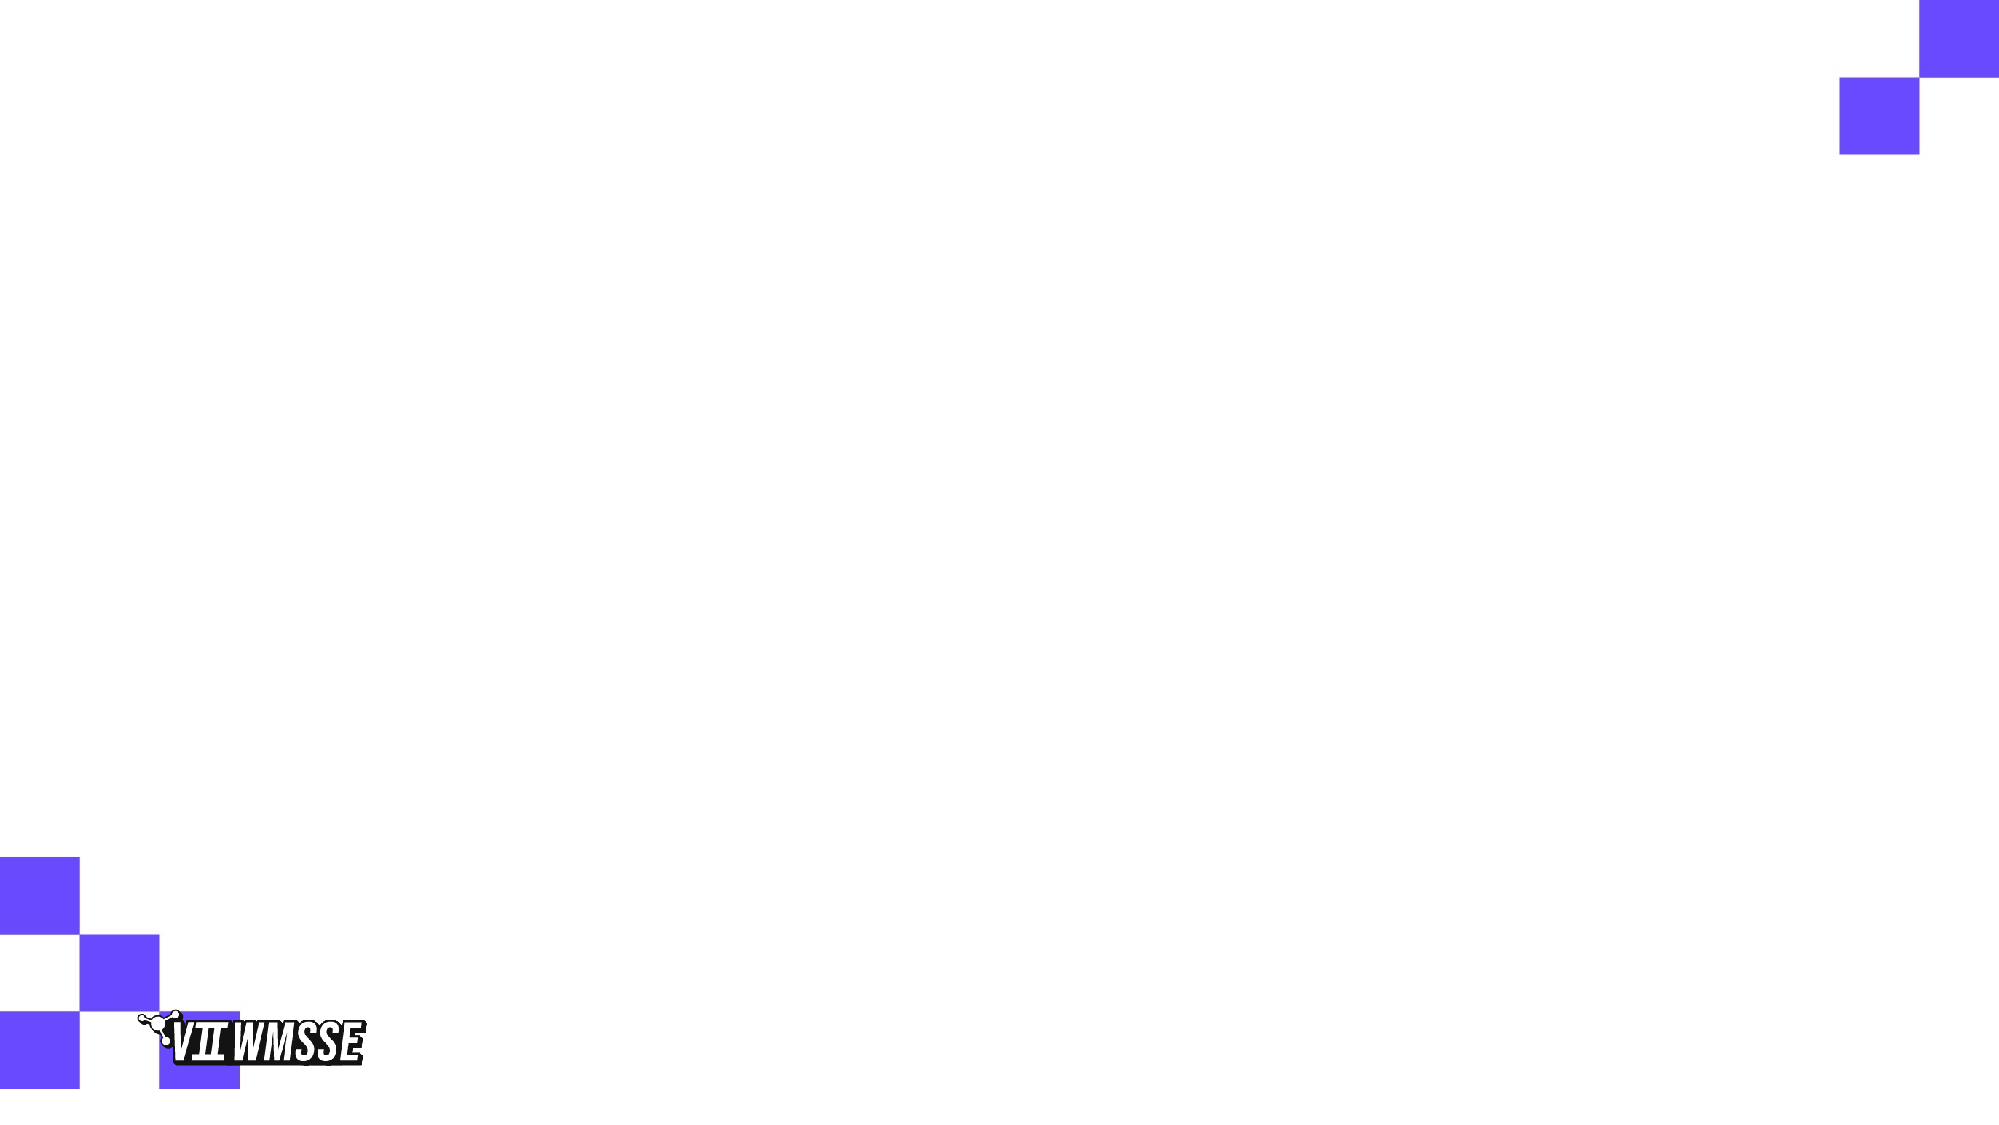
\includegraphics[width=\paperwidth,height=\paperheight]{Fondos/Cuerpo.pdf}}

  % Forzamos color negro
  \setbeamercolor{frametitle}{fg=white}
  \setbeamercolor{normal text}{fg=black}
  \setbeamercolor{structure}{fg=black}
  \setbeamercolor{itemize item}{fg=black}


  \begin{frame}{Longitudes características}
  \begin{columns}[t]
      \begin{column}{0.48\textwidth}
      \vspace{-0.4cm}
        \begin{block}{Parámetro de Ginzburg-Landau $\kappa$}
        \begin{equation*}
            \kappa=\frac{\lambda}{\xi}
        \end{equation*}
            Es una propiedad intrínseca del material. Es el parámetro más importante de GL porque determina el tipo de superconductor:

            \begin{align*}
                \kappa & < \frac{1}{\sqrt{2}} : Tipo \ I & \kappa & >\frac{1}{\sqrt{2}}: Tipo \ II
            \end{align*}
        \end{block}
        \end{column}

        \begin{column}{0.48\textwidth}
        La frontera o pared entre Tipo I y Tipo II viene de la energía de superficie entre una región normal y una superconductora:
            \begin{itemize}
                \item Si $\xi>\lambda$: La pared tiene energía positiva $\rightarrow$ el sistema prefiere minimizar el área de la frontera $\rightarrow$ el campo entra todo de golpe
                \item Si $\xi<\lambda$: La pared  tiene energía negativa $\rightarrow$ el sistema prefiere maximizar el área de la frontera $\rightarrow$ conviene dividir el flujo en vórtices individuales
            \end{itemize}
        \end{column}
    \end{columns}
  \end{frame}
}

%===========================5========================
{
  \usebackgroundtemplate{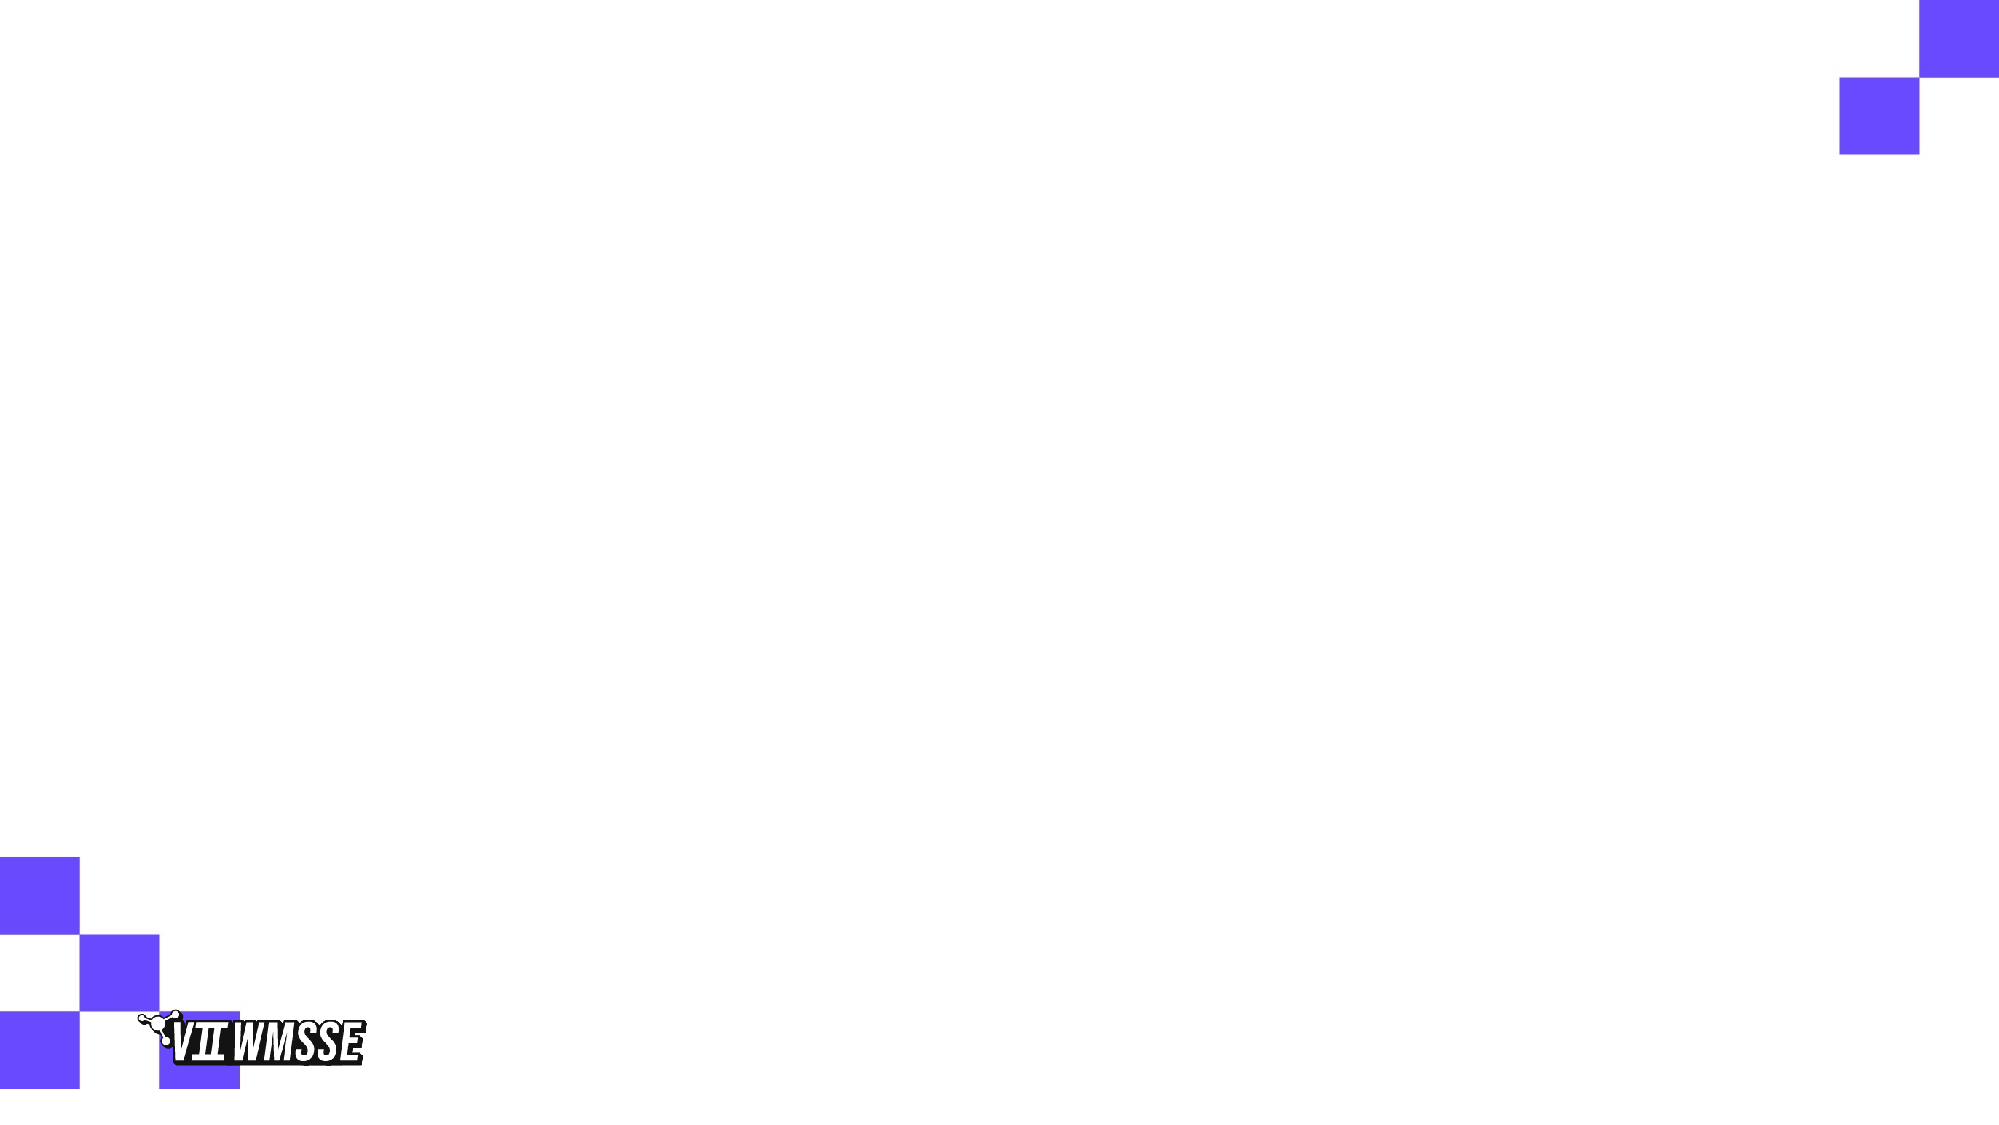
\includegraphics[width=\paperwidth,height=\paperheight]{Fondos/Cuerpo.pdf}}

  % Forzamos color negro
  \setbeamercolor{frametitle}{fg=white}
  \setbeamercolor{normal text}{fg=black}
  \setbeamercolor{structure}{fg=black}
  \setbeamercolor{itemize item}{fg=black}


  \begin{frame}{Ginzburg-Landau Dependiente del Tiempo (TDGL)}
  \vspace{0cm}
    \begin{block}{}
    \begin{equation*}
        \frac{u}{\sqrt{1+\gamma^2\lvert\psi\rvert^2}}\left [ \frac{\partial\psi}{\partial t}+i\mu\psi+\frac{\gamma^2}{2}\frac{\partial\lvert\psi\rvert^2}{\partial t}\psi\right]= (\nabla - iA)^2\psi+\psi(\epsilon(r)-\lvert\psi\lvert^2)
    \end{equation*}
    \end{block}
    \begin{columns}[t]
      \begin{column}{0.48\textwidth}
      \vspace{-0.4cm}
      \begin{block}{Derecha:¿Hacia dónde quiere ir $\psi$?}
          
        \begin{itemize}
            \item El potencial de Landau $\psi(\epsilon-\lvert\psi\rvert^2)$, la función $\epsilon(r)$ es la válvula geométrica de la simulación.
            \item La difusión gauge-invariante $(\nabla-iA)^2\psi$, en presencia de campo se produce el efecto Meissner y las corrientes alrededor de los vórtices.
        \end{itemize}
      \end{block}
    \end{column}

        \begin{column}{0.48\textwidth}
        \vspace{-0.4cm}
            \begin{block}{Izquierda: inercia con que se mueve $\psi$}
                \begin{itemize}
                    \item $\partial\psi/\partial t$: Cambio temporal
                    \item $i\mu\psi$: Acople con el potencial electrostático $\mu$
    
                    \item $\frac{\gamma^2}{2}\frac{\partial\lvert\psi\rvert^2}{\partial t}\psi$ relajación del gap de energía
                    \item $u/{\sqrt{1+\gamma^2\lvert\psi\rvert^2}}$ reduce la velocidad de relajación cuando la densidad de pares es alta
                \end{itemize}
            \end{block}
        \end{column}
    \end{columns}
  \end{frame}
}




{
  \usebackgroundtemplate{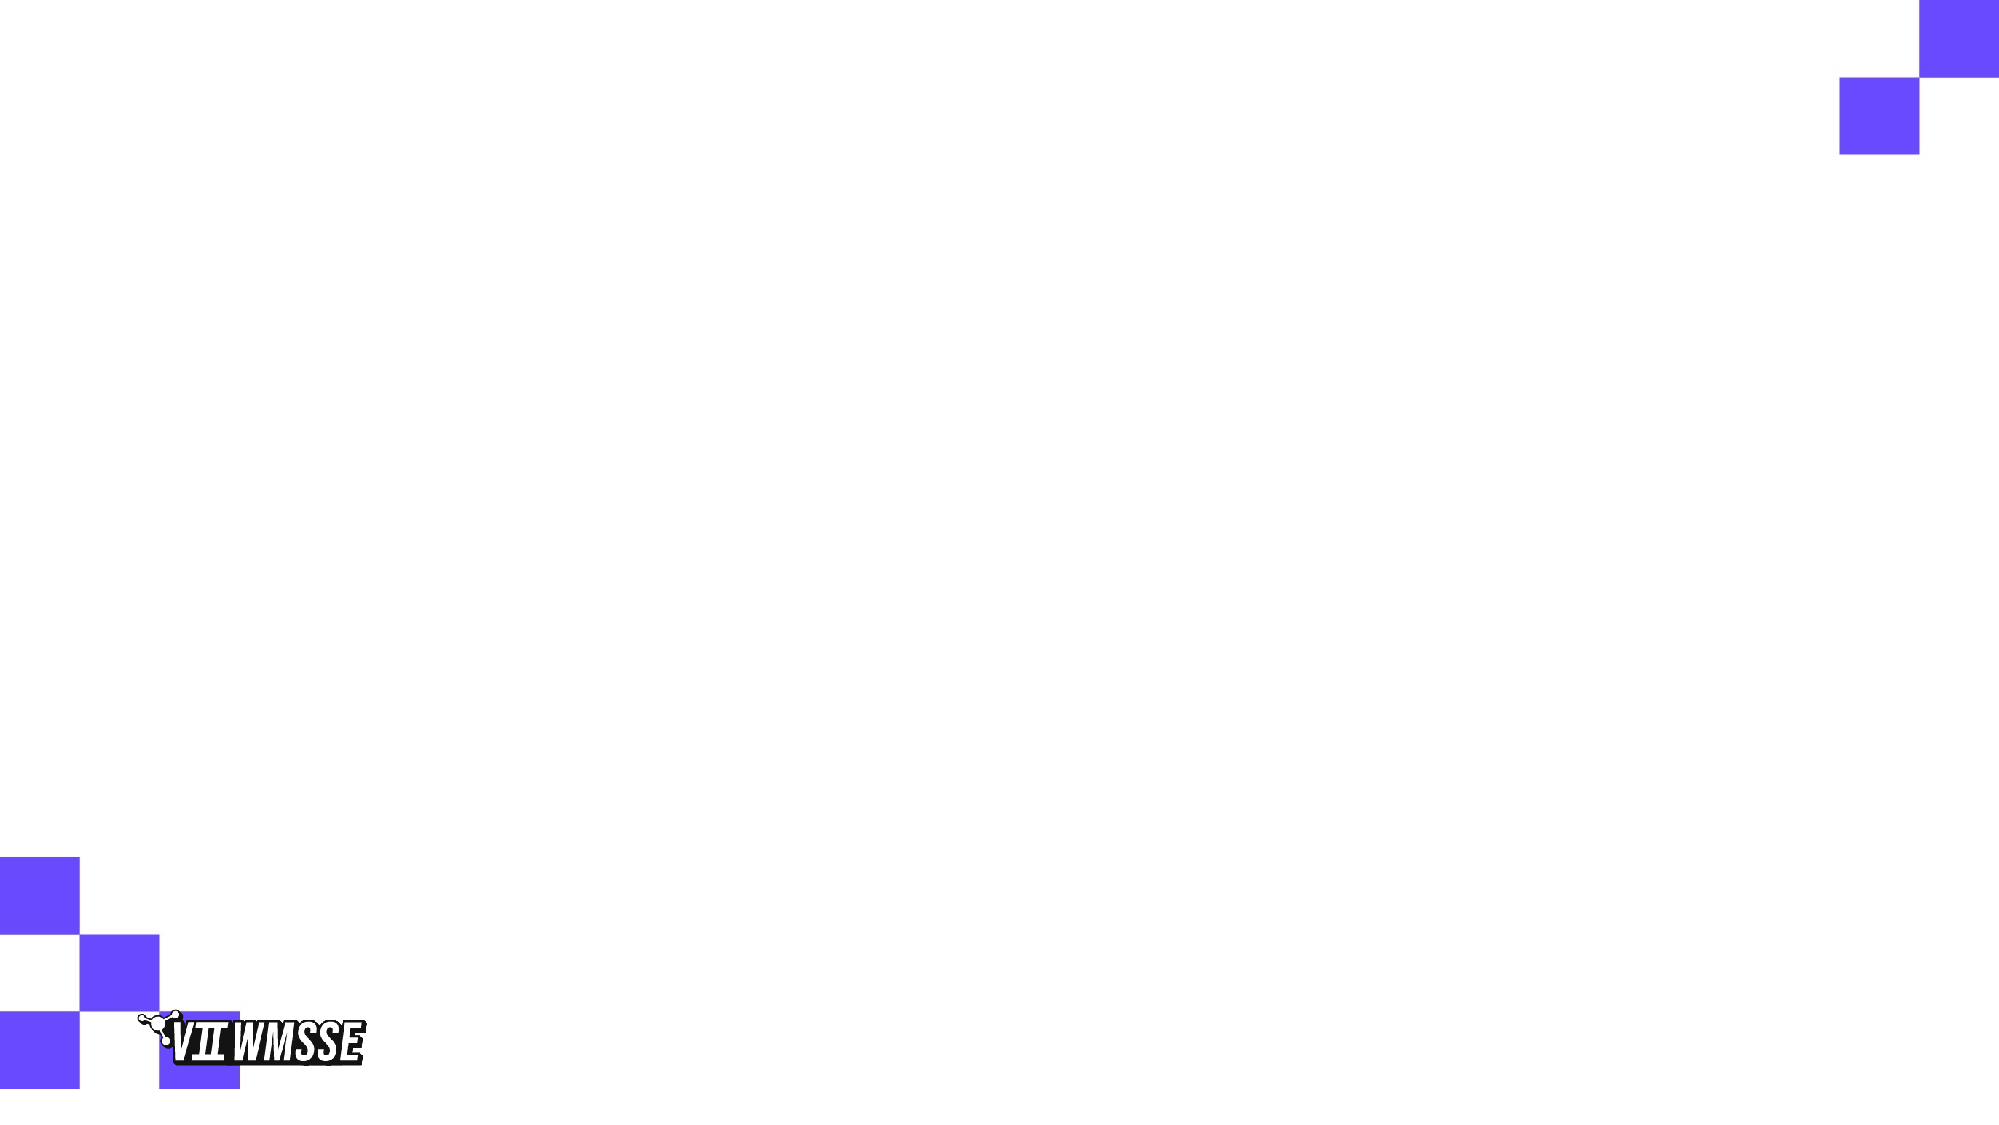
\includegraphics[width=\paperwidth,height=\paperheight]{Fondos/Cuerpo.pdf}}

  % Forzamos color negro
  \setbeamercolor{frametitle}{fg=white}
  \setbeamercolor{normal text}{fg=black}
  \setbeamercolor{structure}{fg=black}
  \setbeamercolor{itemize item}{fg=black}


\begin{frame}{Vórtices: De la Estructura a la Dinámica}
    \scriptsize 

    \begin{columns}[t]
      \begin{column}{0.48\textwidth}
        \begin{block}{Vórtices de Abrikosov (Estáticos)}
          \centering
          \begin{itemize}
            \item \textbf{Origen}: Estado fundamental en superconductores tipo-II ante un campo $H > H_{c1}$.
            \item \textbf{Estructura}: Núcleo normal rodeado por supercorrientes de apantallamiento.
            \item \textbf{Rol}: Definen la 'red de vórtices' que interactúa con las geometrías de anclaje.
          \end{itemize}
        \end{block}
      \end{column}

      \begin{column}{0.48\textwidth}
        \begin{block}{Vórtices Cinemáticos (Dinámicos)}
          \centering
          \begin{itemize}
            \item \textbf{Origen}: Desplazamiento forzado de vórtices por fuerza de Lorentz ($F_L = j \times B$).
            \item \textbf{Estructura}: Estado disipativo temporal donde se rompe la fase superconductora local.
            \item \textbf{Rol}: Generan el voltaje resistivo ($R_{flow}$) responsable de la no-linealidad en el diodo.
          \end{itemize}
        \end{block}
      \end{column}
    \end{columns}

    \vspace{0.4cm}
    \centering
    \textit{La rectificación en el SDE surge de la competencia entre el anclaje de vórtices de Abrikosov y el movimiento de los vórtices cinemáticos.}
  \end{frame}
}








%===========================5========================

{
  \usebackgroundtemplate{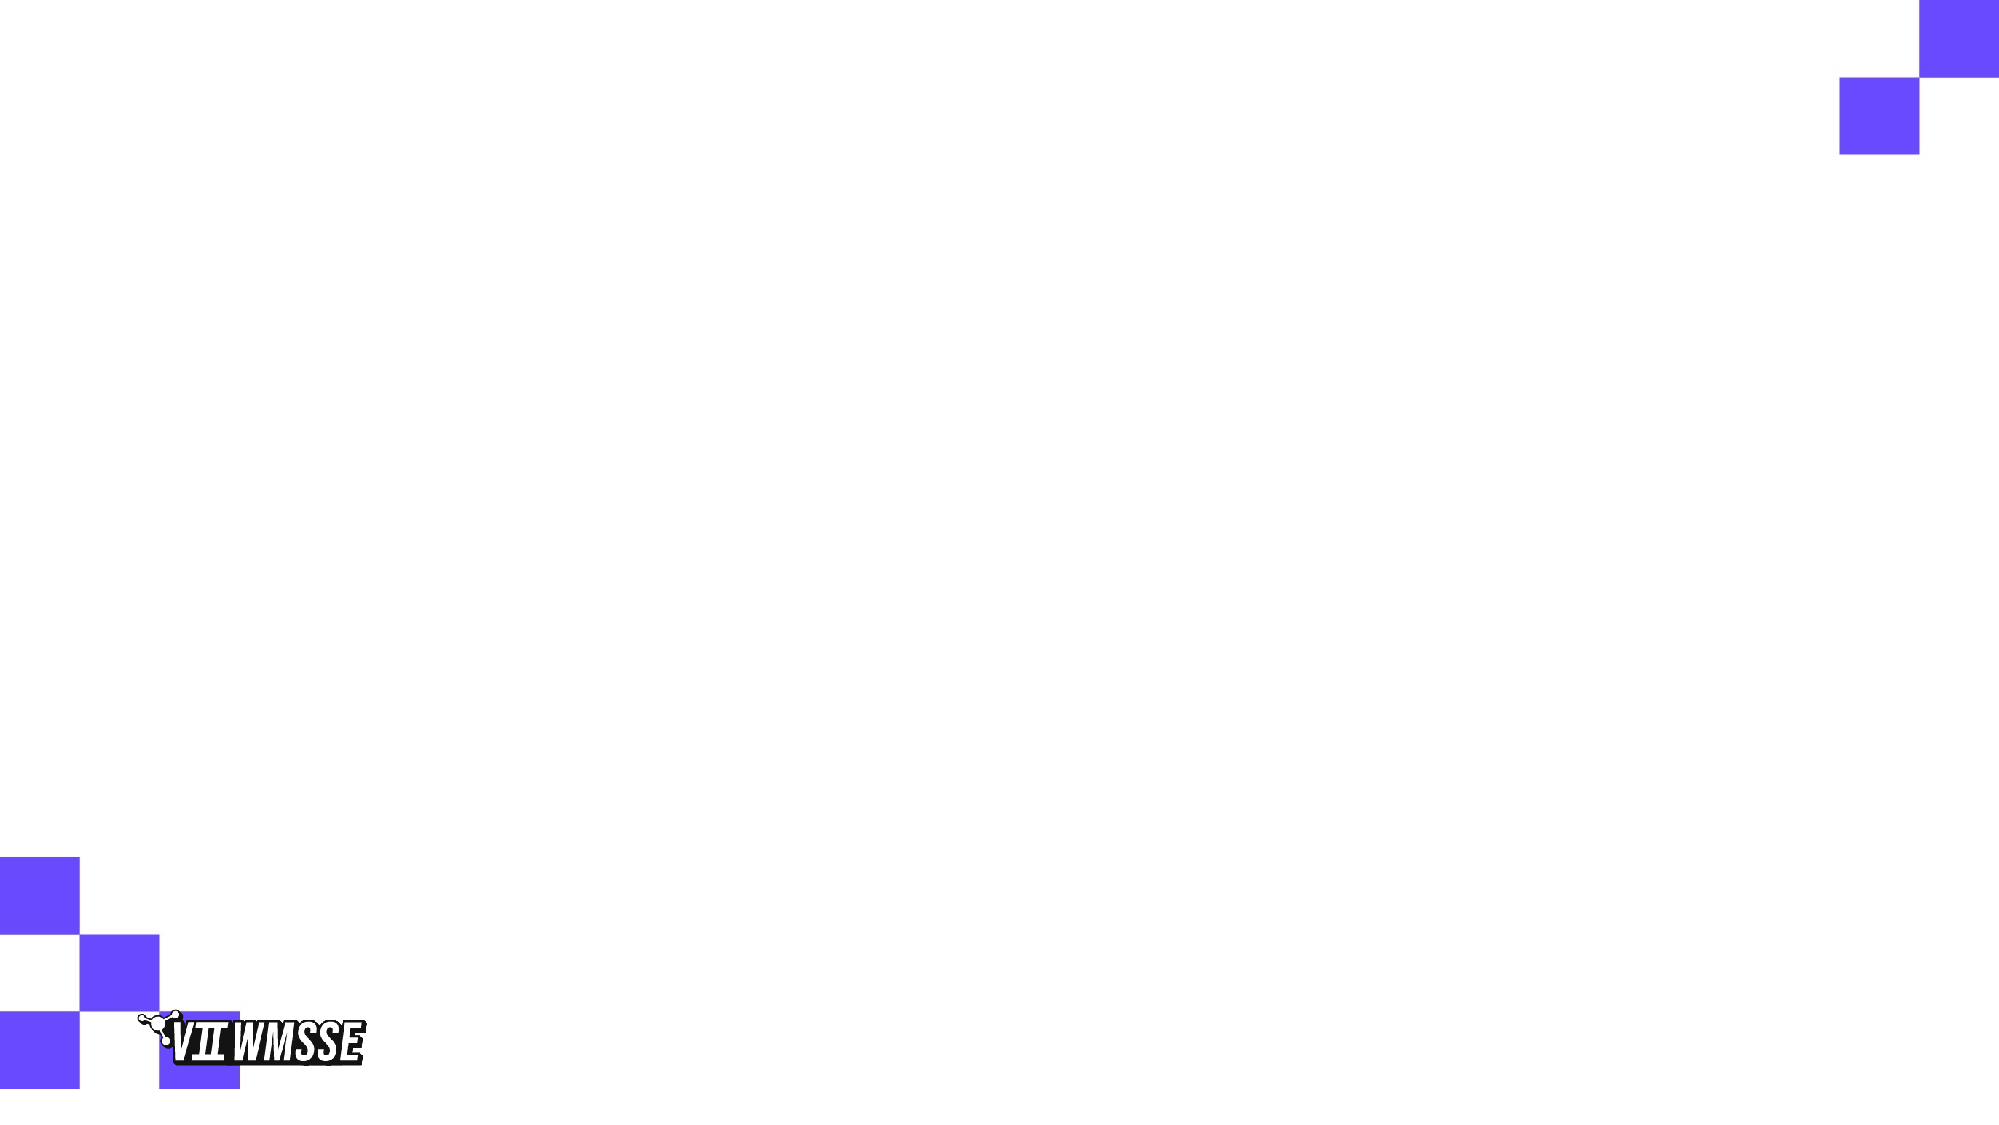
\includegraphics[width=\paperwidth,height=\paperheight]{Fondos/Cuerpo.pdf}}

  % Forzamos color negro
  \setbeamercolor{frametitle}{fg=white}
  \setbeamercolor{normal text}{fg=black}
  \setbeamercolor{structure}{fg=black}
  \setbeamercolor{itemize item}{fg=black}

\begin{frame}{El Diodo}
    \scriptsize
    % Cambiamos [t] por [c] para centrar verticalmente toda la diapositiva
    \begin{columns}[c]

      % COLUMNA IZQUIERDA
\begin{column}{0.48\textwidth}
        \centering
        \vfill 
        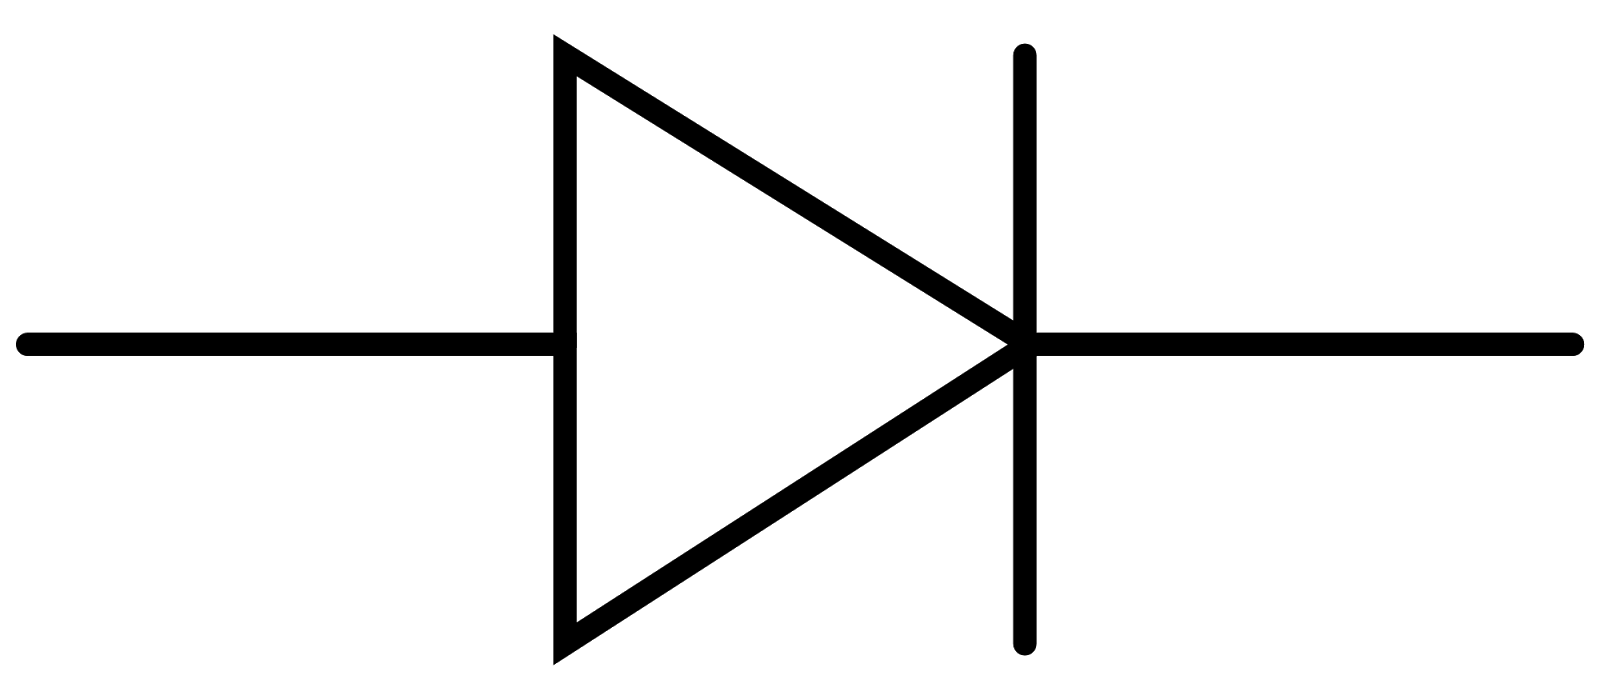
\includegraphics[width=0.8\linewidth]{Imagenes/diodo.png}
        \\[0.2cm]
        \textit{Figura: Representación del Diodo}
        \vfill 
      \end{column}

      % COLUMNA DERECHA
      \begin{column}{0.48\textwidth}
        \begin{block}{Diodo Semiconductor (Unión p-n)}
          \centering
          Basado en barrera electrostática.
        \end{block}
        
        \vspace{0.2cm}
        
        \begin{itemize}
          \item \textbf{Región p}: Exceso de huecos (+).
          \item \textbf{Región n}: Exceso de electrones (-).
          \item \textbf{Limitación}: Caída de tensión fija ($V \approx 0.7V$) $\rightarrow$ \textbf{Efecto Joule} inevitable.
        \end{itemize}
        
        \vspace{0.5cm}
        \centering
        \textit{La unión p-n disipa calor por naturaleza; el diodo de vórtices lo anula.}
      \end{column}

    \end{columns}
  \end{frame}
}







%==========================6=========================
%=================================================
% DIAPOSITIVA: ¿Por Qué Necesitamos el Diodo Superconductor?
%=================================================
{
  \usebackgroundtemplate{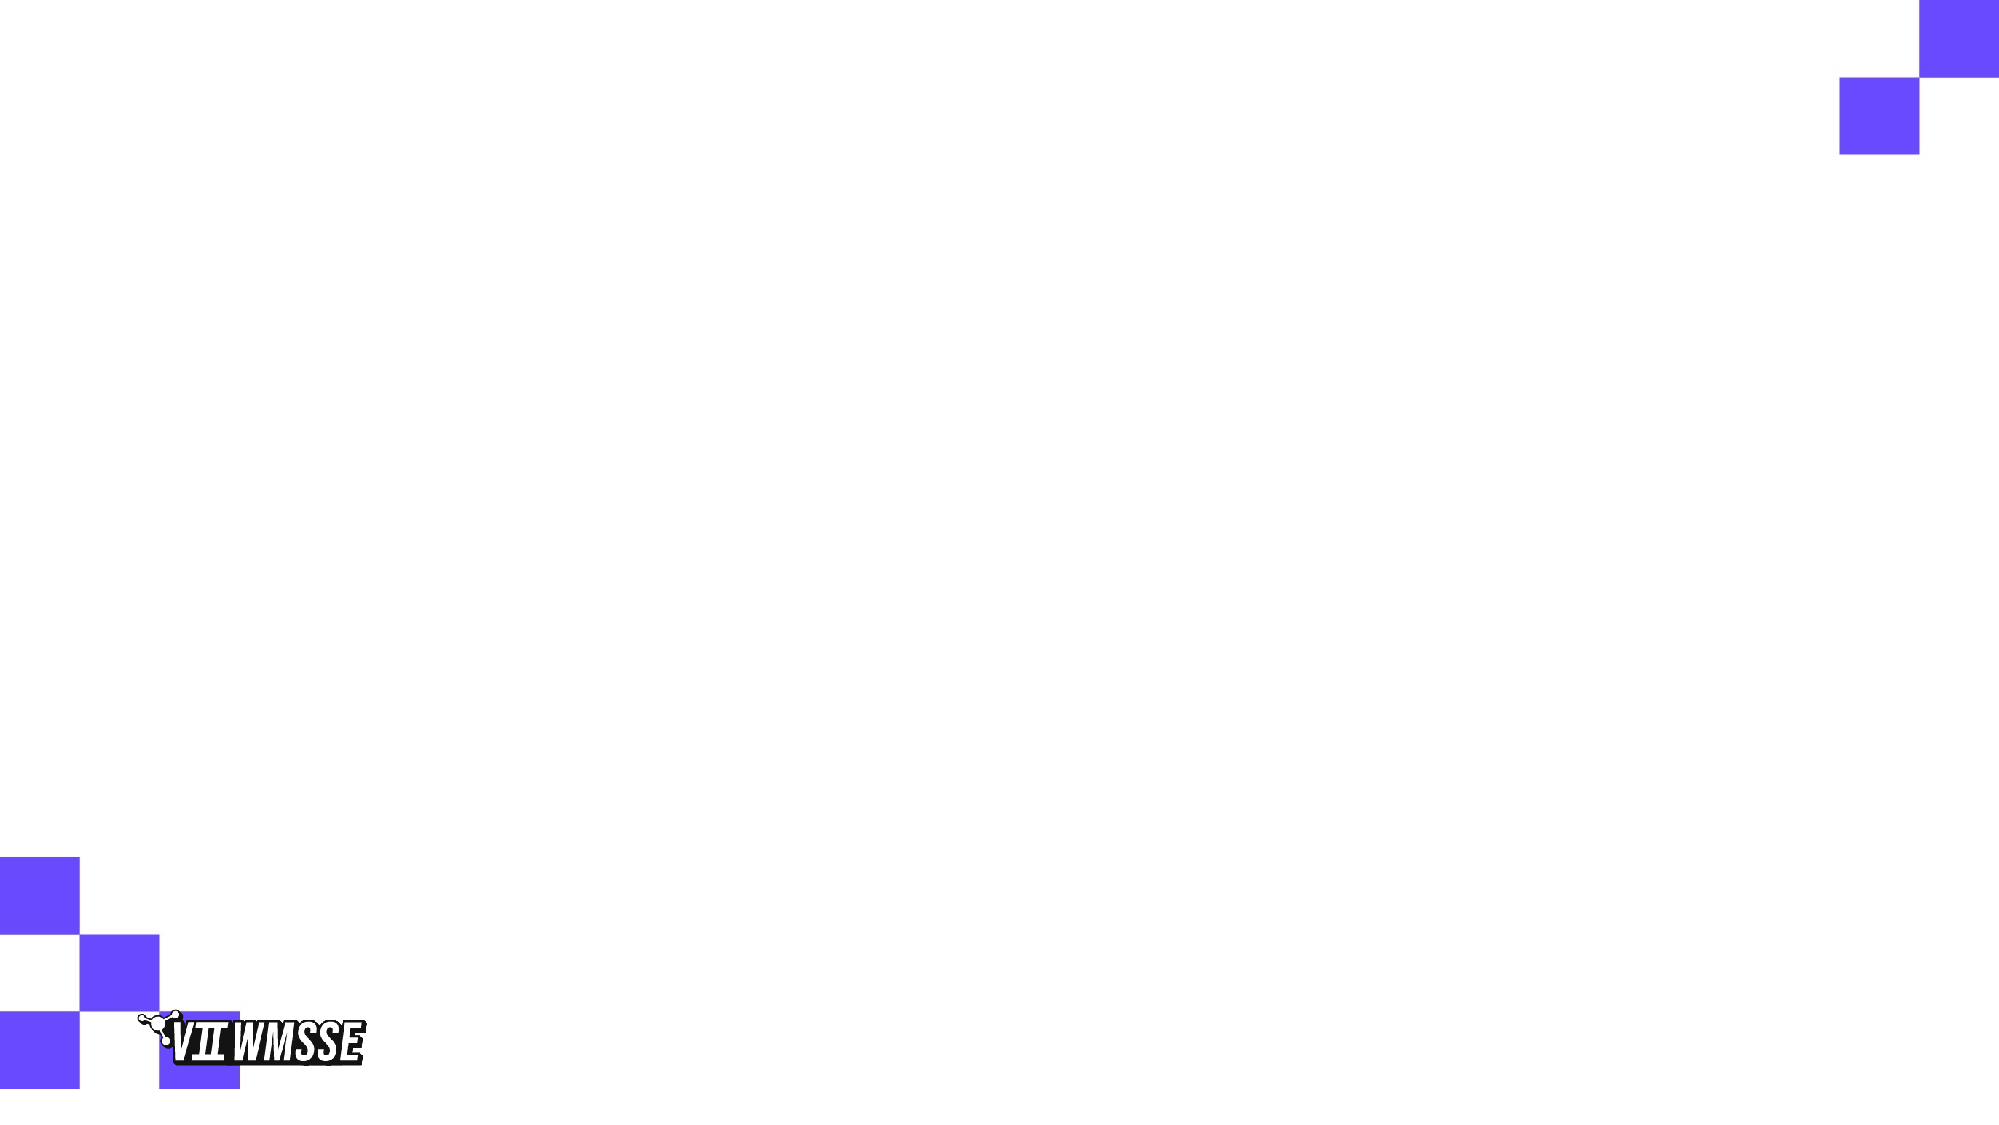
\includegraphics[width=\paperwidth,height=\paperheight]{Fondos/Cuerpo.pdf}}
  \setbeamercolor{frametitle}{fg=white}
  \setbeamercolor{normal text}{fg=black}
  \setbeamercolor{structure}{fg=black}

  \begin{frame}{El Gasto Energético de la Refrigeración}
    \framesubtitle{}
    \scriptsize
    \begin{columns}[t]
      \begin{column}{0.48\textwidth}
        \begin{block}{Escala de la Demanda (TWh)}
          \centering
          \begin{tabular}{lc}
            \hline
            \textbf{Año} & \textbf{Consumo Global} \\ \hline
            2024 (Base) & 415 - 460 \\
            2030 (Proj.) & 945 - 1.065 \\
            2035 (Límite) & 1.300 \\ \hline
          \end{tabular}
        \end{block}
        \begin{itemize}
          \item \textbf{Costo IA}: GPT-4 requiere 50 GWh/entrenamiento (40k hogares/año).
          \item \textbf{Ineficiencia}: ~40\% de la energía se pierde exclusivamente en disipar calor (PUE ineficiente).
        \end{itemize}
      \end{column}

      \begin{column}{0.48\textwidth}
        \begin{block}{Crisis Hídrica y Local}
          \centering
          \vspace{0.1cm}
          IA Generativa: 500 ml de agua evaporada por cada 100 palabras redactadas.
        \end{block}
        \begin{itemize}
          \item \textbf{Canelones, Uruguay}: Google proyectó 7,6M de litros/día (consumo de 55,000 hab).
          \item \textbf{Clementina XXI}: Limitaciones estructurales en Argentina por demanda de potencia ($P_{TDP} = 600W/chip$).
        \end{itemize}
      \end{column}
    \end{columns}
  \end{frame}
}



{
  \usebackgroundtemplate{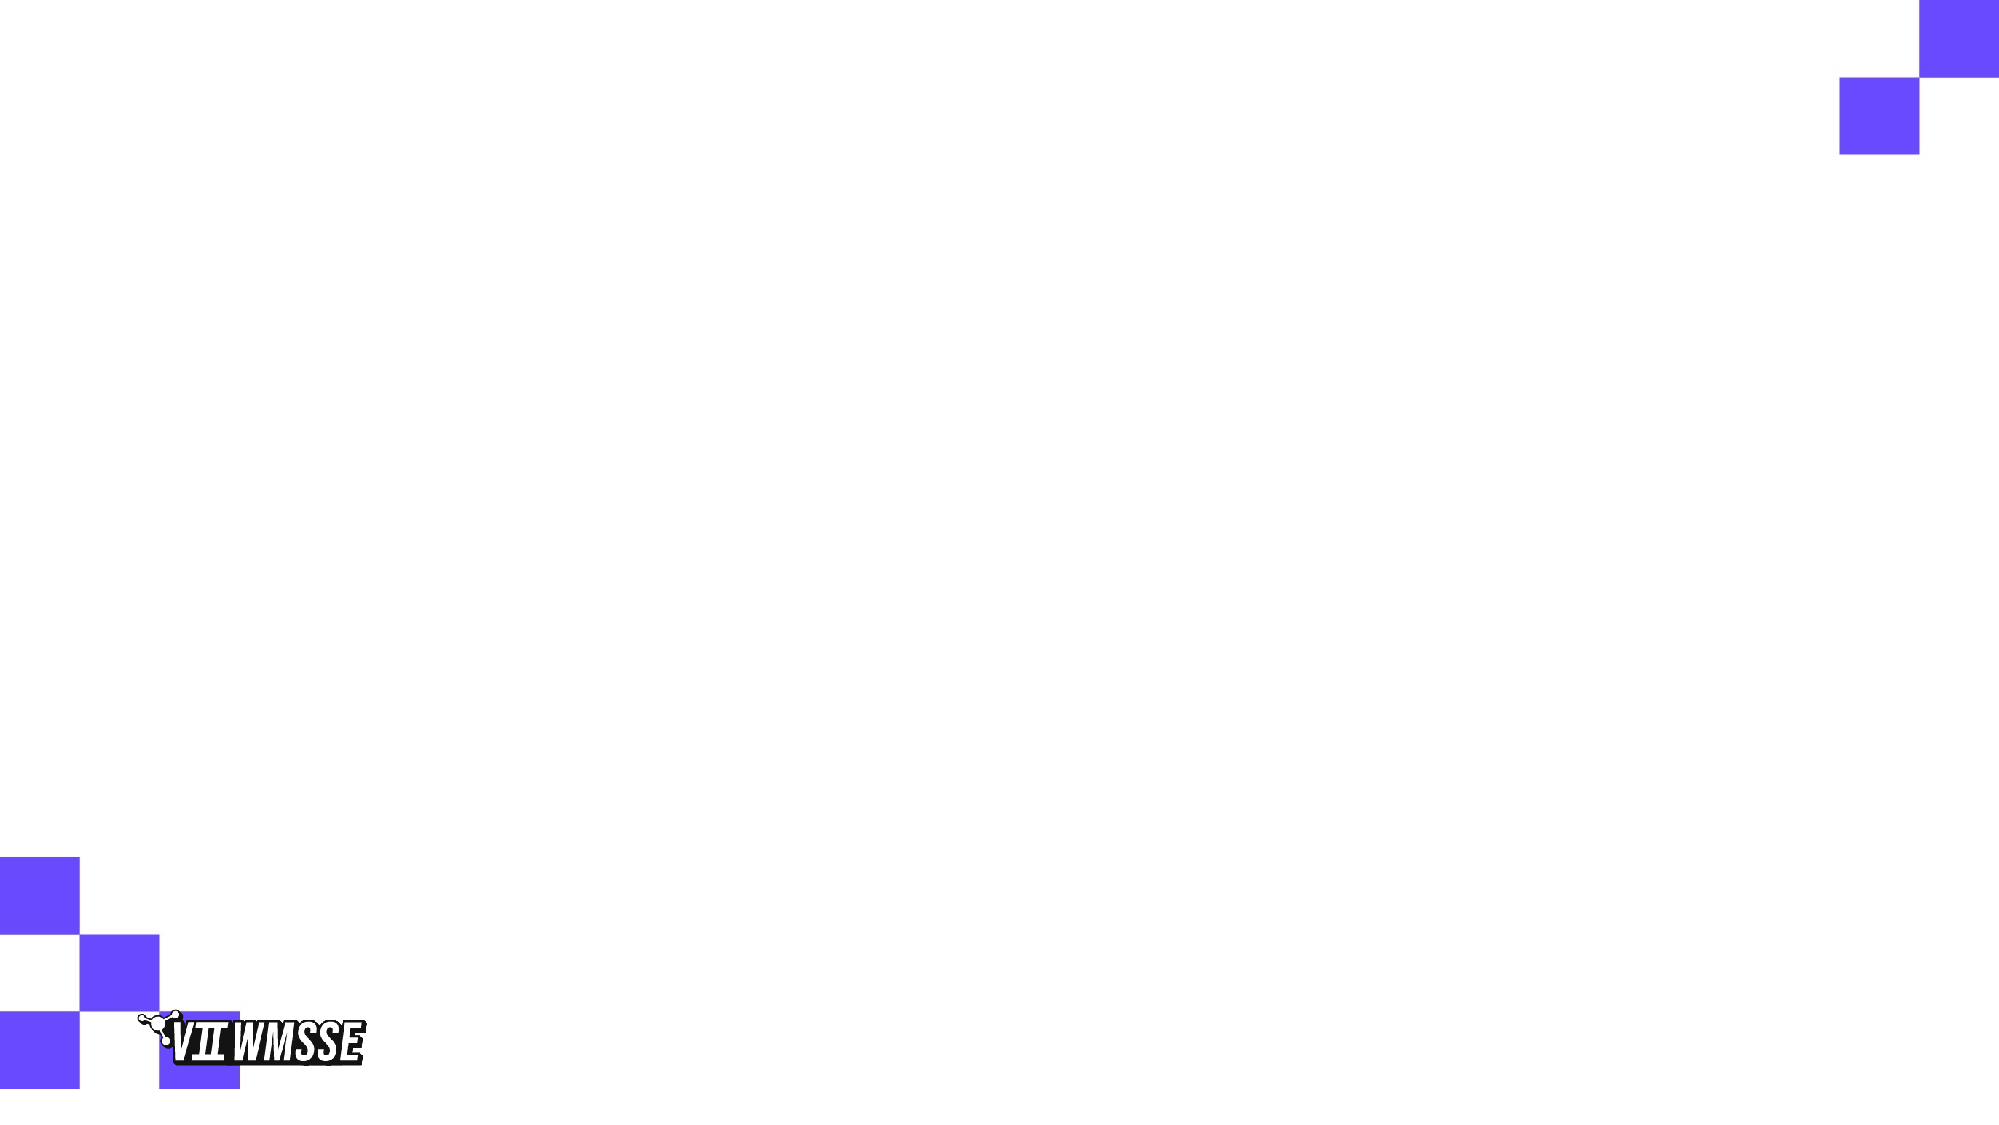
\includegraphics[width=\paperwidth,height=\paperheight]{Fondos/Cuerpo.pdf}}
  \setbeamercolor{frametitle}{fg=white}
  \setbeamercolor{normal text}{fg=black}
  \setbeamercolor{structure}{fg=black}

  \begin{frame}{La Solución en la Superconducción}
    \framesubtitle{}
    \scriptsize
    \begin{columns}[t]
      \begin{column}{0.48\textwidth}
        \begin{block}{Control del Efecto Diodo (SDE)}
          \centering
          Basado en ecuaciones gTDGL:
          \[ \text{Ruptura de simetría: IRS + TRS} \]
          \vspace{-0.2cm}
          \begin{itemize}
            \item \textbf{Optimización}: Resonancia entre profundidad de penetración ($\lambda_L$) y red de vórtices.
            \item \textbf{Geometría}: Uso de 'peines' asimétricos para controlar el anclaje de vórtices.
          \end{itemize}
        \end{block}
      \end{column}

      \begin{column}{0.48\textwidth}
        \begin{block}{Desacople Termodinámico}
          \centering
          \begin{tabular}{l|c|c}
            \textbf{Atributo} & \textbf{Semiconductor} & \textbf{SDE} \\ \hline
            Resistencia ($R$) & $R > 0$ & $R = 0$ \\
            Calor ($P$) & $V \cdot I$ & $0$ \\
            Frecuencia & GHz & THz \\ \hline
          \end{tabular}
        \end{block}
        \centering
        \vspace{0.2cm}
        \textit{La implementación de diodos de vórtices permite lógica digital sin disipación Joule, rompiendo el ciclo de refrigeración activa.}
      \end{column}
    \end{columns}
  \end{frame}
}


%===============================7====================
{
  \usebackgroundtemplate{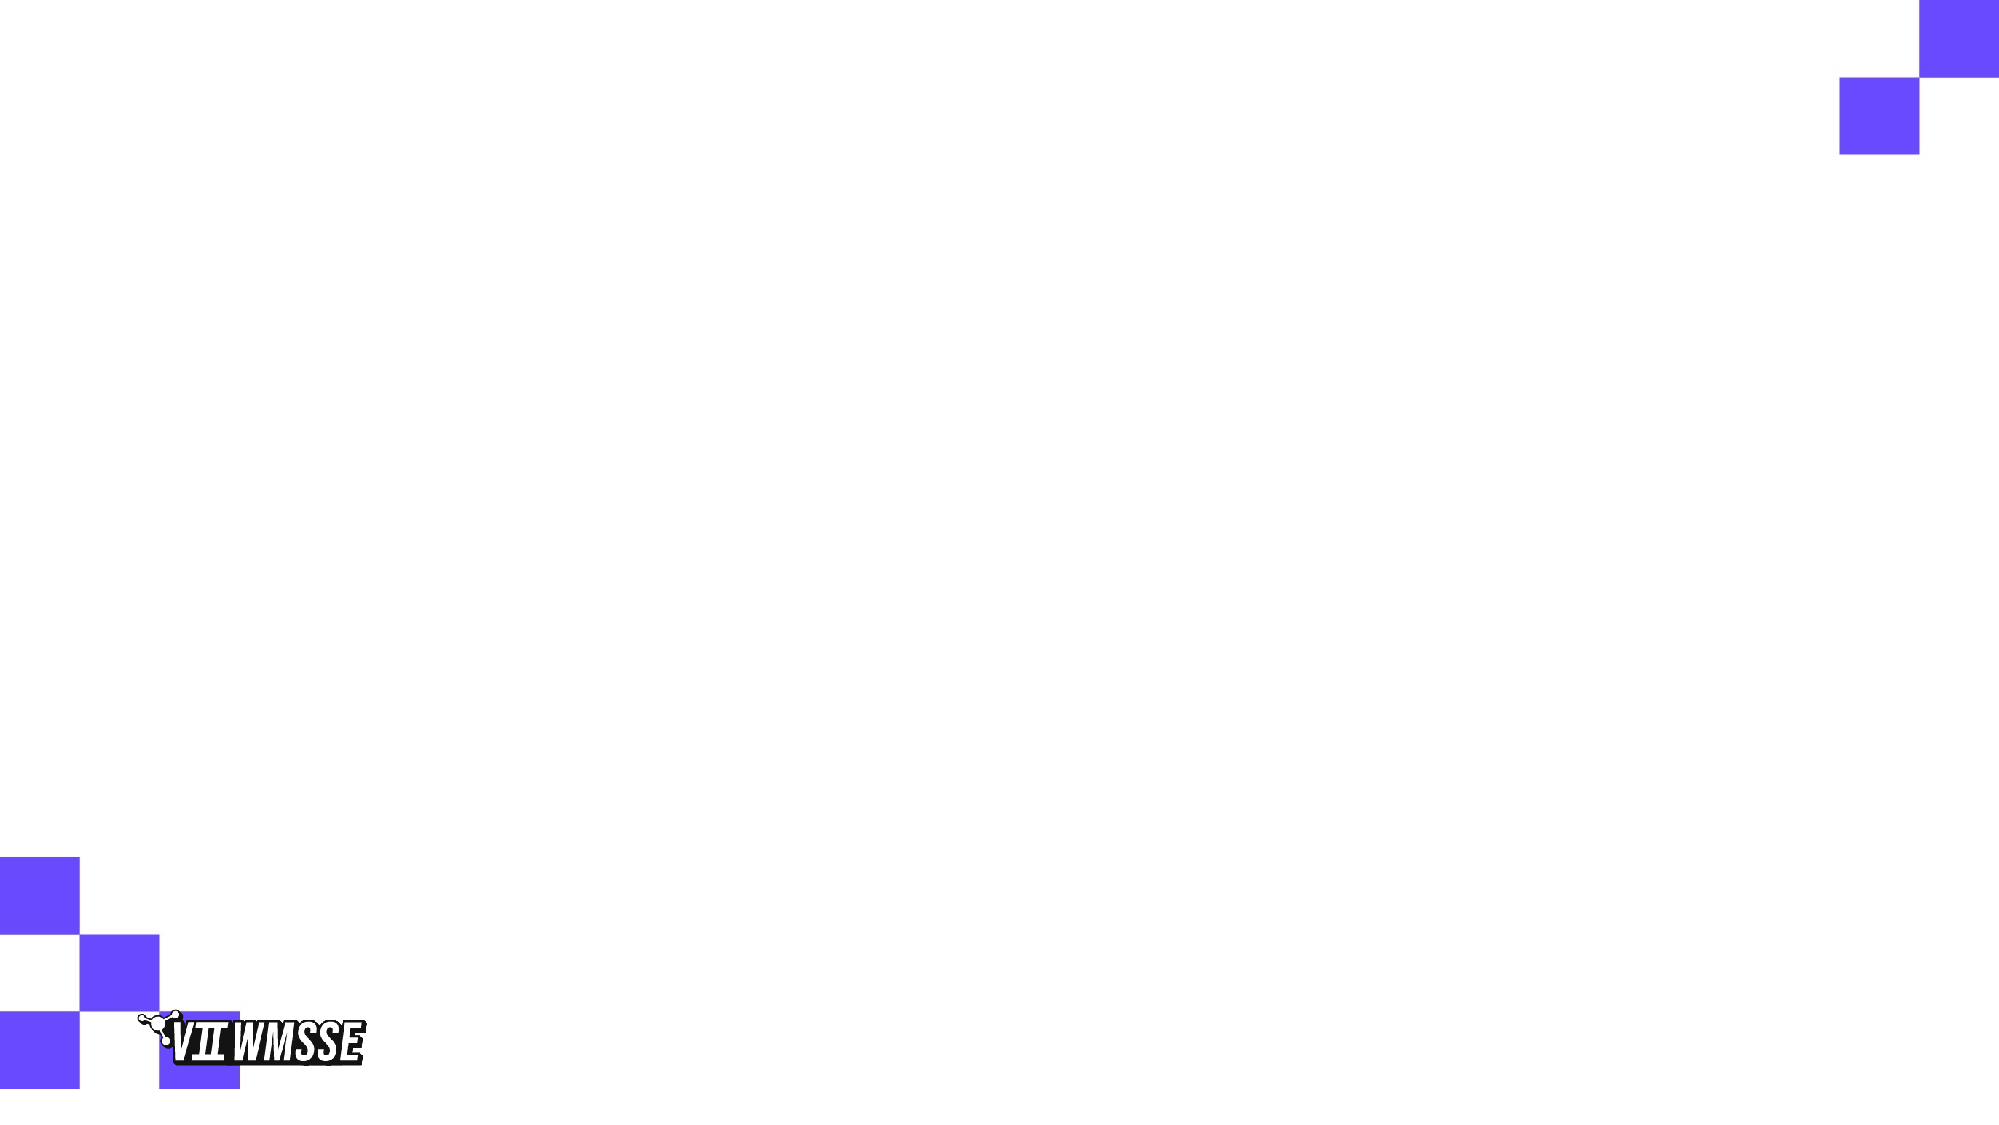
\includegraphics[width=\paperwidth,height=\paperheight]{Fondos/Cuerpo.pdf}}

  % Forzamos color negro
  \setbeamercolor{frametitle}{fg=white}
  \setbeamercolor{normal text}{fg=black}
  \setbeamercolor{structure}{fg=black}
  \setbeamercolor{itemize item}{fg=black}

\section{Geometría, Parámetros y Simulación}
  \begin{frame}{Geometría}
    \framesubtitle{Subtítulo aquí}

    \begin{columns}[c]

        % Columna izquierda
        \begin{column}{0.58\textwidth}
             \centering
            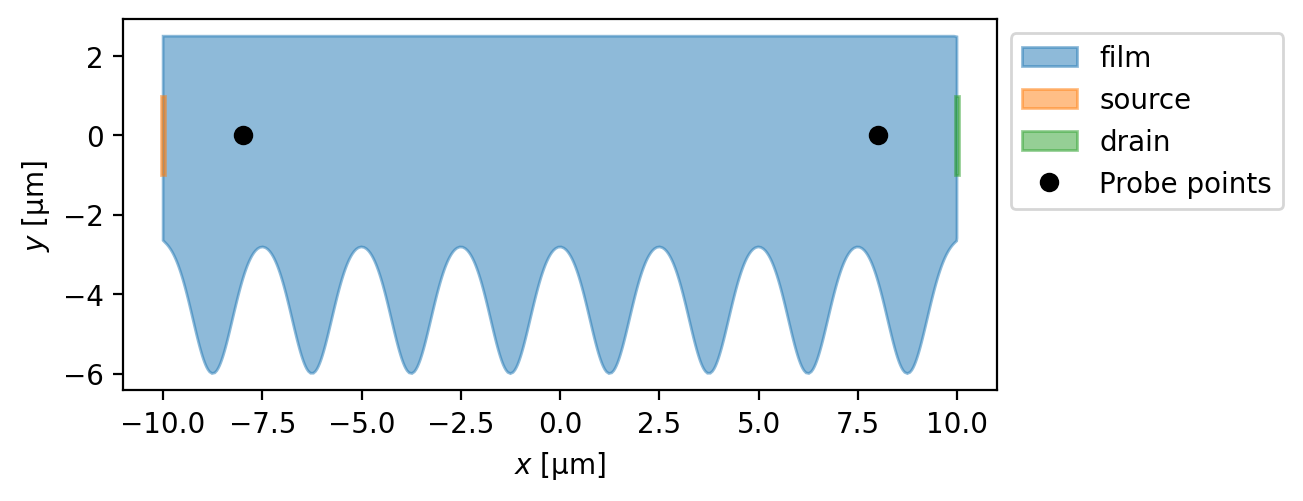
\includegraphics[width=1\linewidth]{Imagenes/Geometria.png}

        \end{column}

        % Columna derecha
        \begin{column}{0.38\textwidth}

            \small

            \[
            y(x)= -h_d \sum_{i=1}^{N}
            \exp\left[
            -\frac{(x-x_i)^2}{2\delta^2}
            \right]
            \]

            \vspace{0.3cm}

            \[
            \delta = 0.20\Delta x
            \]

            \vspace{0.4cm}

            \begin{itemize}
                \item Perfil inferior generado por gaussianas.
                \item $N$: número de dientes.
                \item Ruptura de simetría $\Rightarrow$ SDE.
            \end{itemize}

        \end{column}

    \end{columns}

\end{frame}
}

%=================================================
% BLOQUE 1: Parámetros de simulación
%=================================================
{
  \usebackgroundtemplate{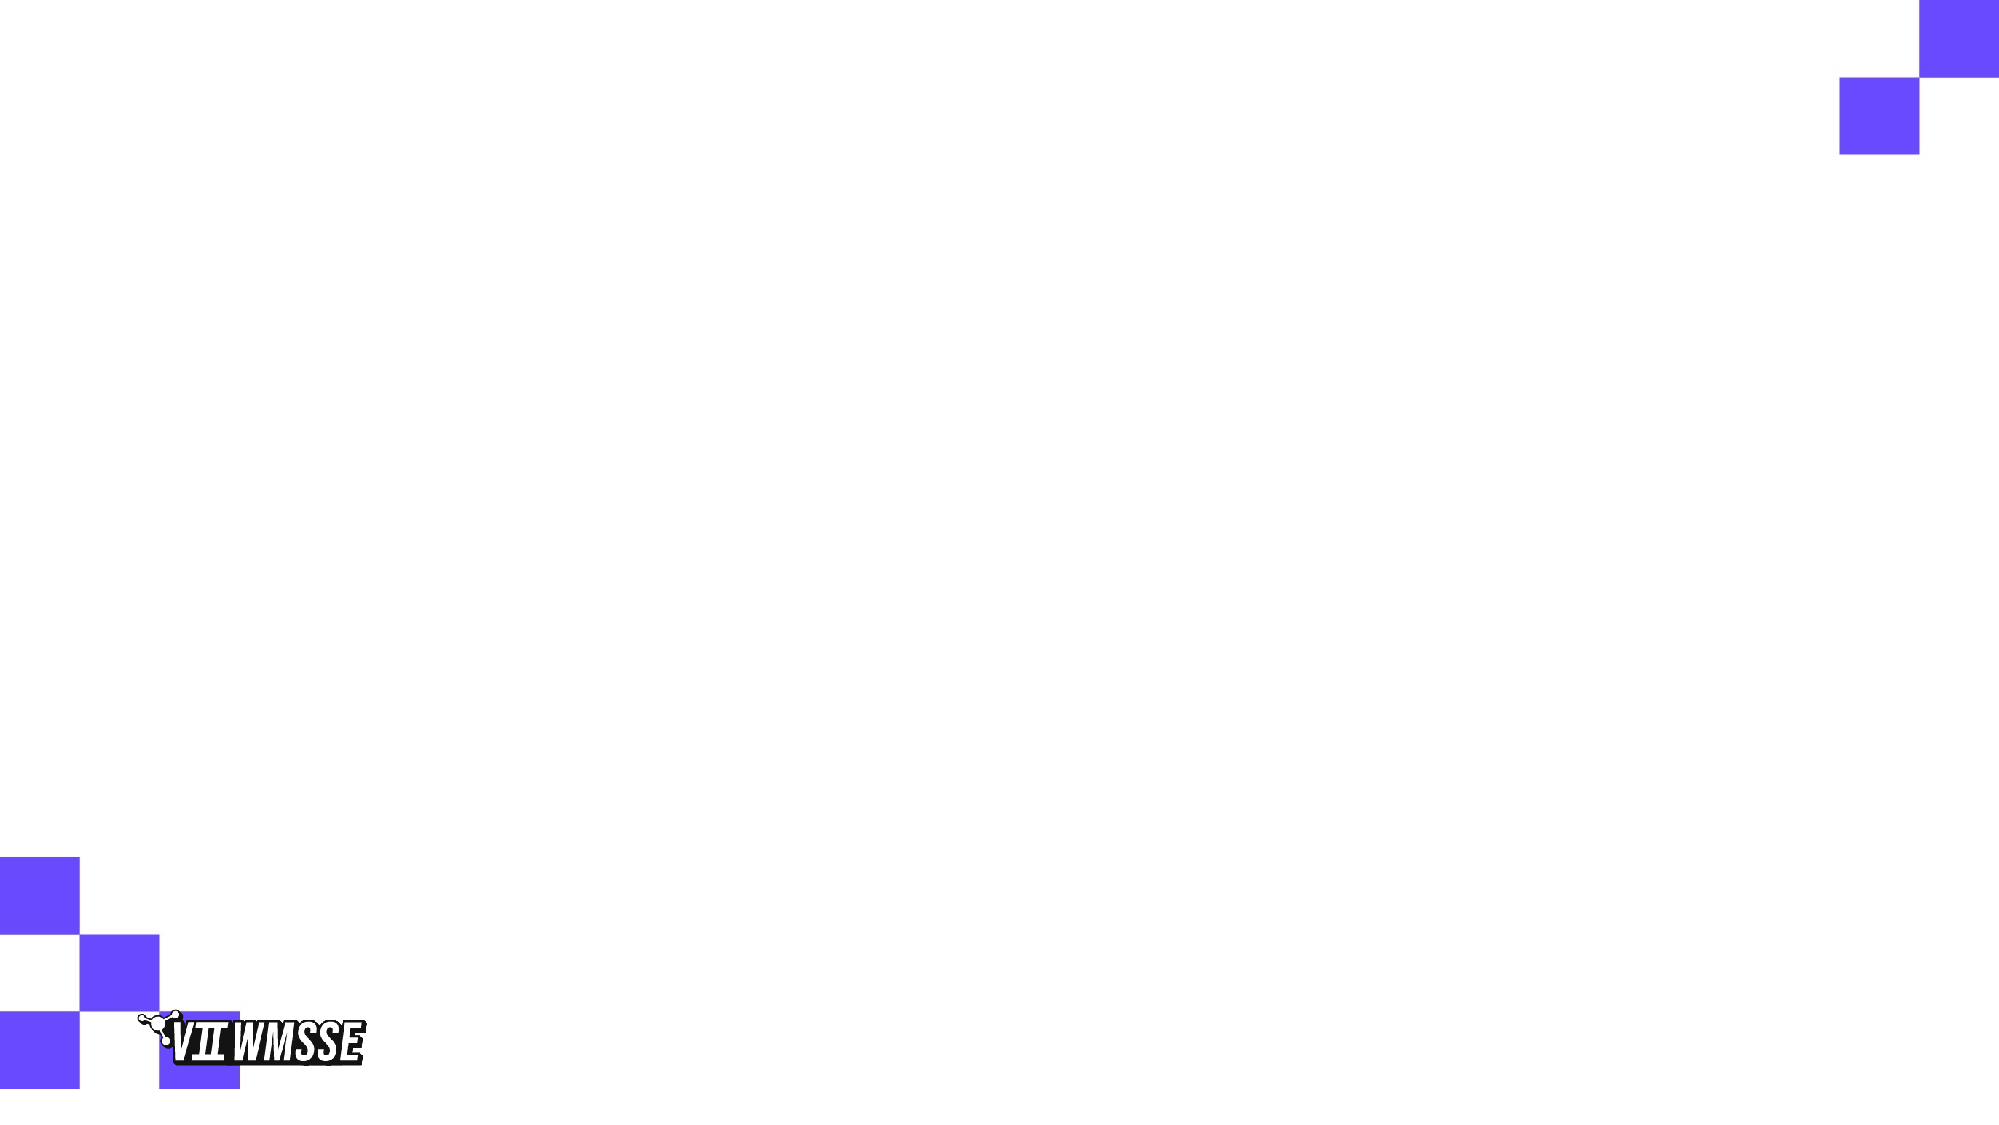
\includegraphics[width=\paperwidth,height=\paperheight]{Fondos/Cuerpo.pdf}}
  \setbeamercolor{frametitle}{fg=white}
  \setbeamercolor{normal text}{fg=black}
  \setbeamercolor{structure}{fg=black}
  \setbeamercolor{itemize item}{fg=black}

  \begin{frame}{Parámetros de Simulación}
    \scriptsize 

    \begin{columns}[t]
      \begin{column}{0.48\textwidth}
        \begin{block}{\centering Material}
          \centering
          \begin{tabular}{lc}
            \hline
            \textbf{Parámetro} & \textbf{Valor} \\
            \hline
            $\xi$ & $0.5~\mu m$ \\
            $\lambda_L$ & $2.0~\mu m$ \\
            $d$ & $0.1~\mu m$ \\
            $\gamma$ & $1.0$ \\
            \hline
          \end{tabular}
        \end{block}
        \centering\textit{Tabla: Propiedades del material.}
      \end{column}

      \begin{column}{0.48\textwidth}
        \begin{block}{\centering Configuración simulada}
          \centering
          \begin{tabular}{lc}
            \hline
            \textbf{Parámetro} & \textbf{Valor} \\
            \hline
            $N$ dientes & $2$ \\
            $B$ & $0.0-1.2~mT$ \\
            Polaridades & $\pm$ \\
            \hline
          \end{tabular}
        \end{block}
        \centering\textit{Tabla: Parámetros de configuración.}
      \end{column}
    \end{columns}
  \end{frame}
}

%=================================================
% BLOQUE 2: Parámetros numéricos y geométricos
%=================================================
{
  \usebackgroundtemplate{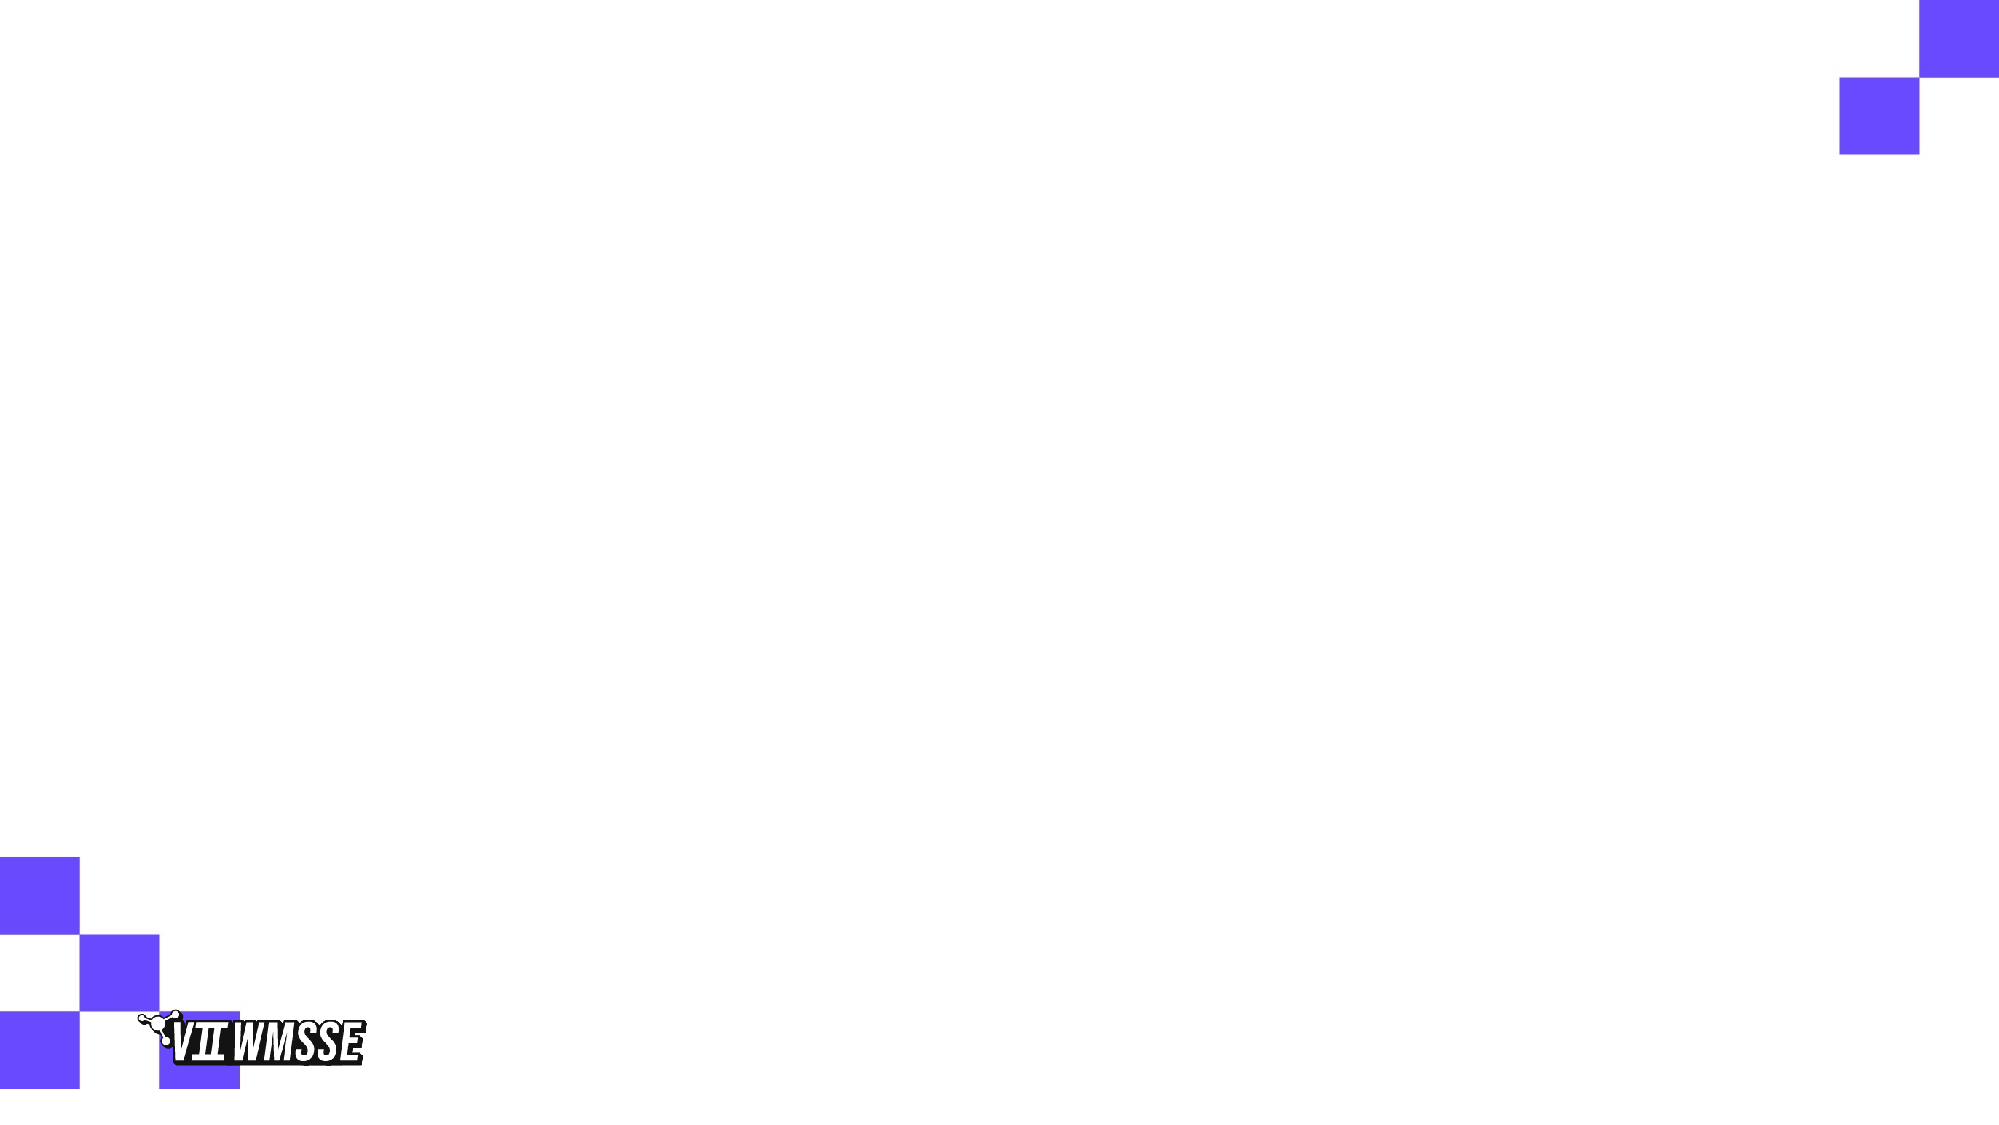
\includegraphics[width=\paperwidth,height=\paperheight]{Fondos/Cuerpo.pdf}}
  \setbeamercolor{frametitle}{fg=white}
  \setbeamercolor{normal text}{fg=black}
  \setbeamercolor{structure}{fg=black}
  \setbeamercolor{itemize item}{fg=black}

  \begin{frame}{Parámetros Numéricos y Geométricos}
    \scriptsize 

    \begin{columns}[t]
      \begin{column}{0.48\textwidth}
        \begin{block}{\centering Geometría}
          \centering
          \begin{tabular}{lc}
            \hline
            \textbf{Parámetro} & \textbf{Valor} \\
            \hline
            $L_x$ & $20.0~\mu m$ \\
            $L_y$ & $5.0~\mu m$ \\
            $h_d$ & $3.5~\mu m$ \\
            $L_y-h_d$ & $1.5~\mu m$ \\
            $L_c$ & $5.0~\mu m$ \\
            $w_c$ & $0.1~\mu m$ \\
            \hline
          \end{tabular}
        \end{block}
        \centering\textit{Tabla: Dimensiones físicas del sistema.}
      \end{column}

      \begin{column}{0.48\textwidth}
        \begin{block}{\centering Barrido de corriente}
          \centering
          \begin{tabular}{lc}
            \hline
            \textbf{Parámetro} & \textbf{Valor} \\
            \hline
            $I_{\min}$ & $-50~\mu A$ \\
            $I_{\max}$ & $50~\mu A$ \\
            $\Delta I$ & $1~\mu A$ \\
            Puntos & $100$ \\
            \hline
          \end{tabular}
        \end{block}
        \centering\textit{Tabla: Rango y resolución del barrido.}

        \vspace{0.25cm}

        \begin{block}{\centering Solver}
          \centering
          \begin{tabular}{lc}
            \hline
            \textbf{Parámetro} & \textbf{Valor} \\
            \hline
            skip\_time & $50$ \\
            solve\_time & $100$ \\
            $h_{\max}$ & $0.25~\mu m$ \\
            \hline
          \end{tabular}
        \end{block}
        \centering\textit{Tabla: Configuración del solver.}
      \end{column}
    \end{columns}
  \end{frame}
}
%=================================================
% BLOQUE 10: Implementación computacional
%=================================================
{
  \usebackgroundtemplate{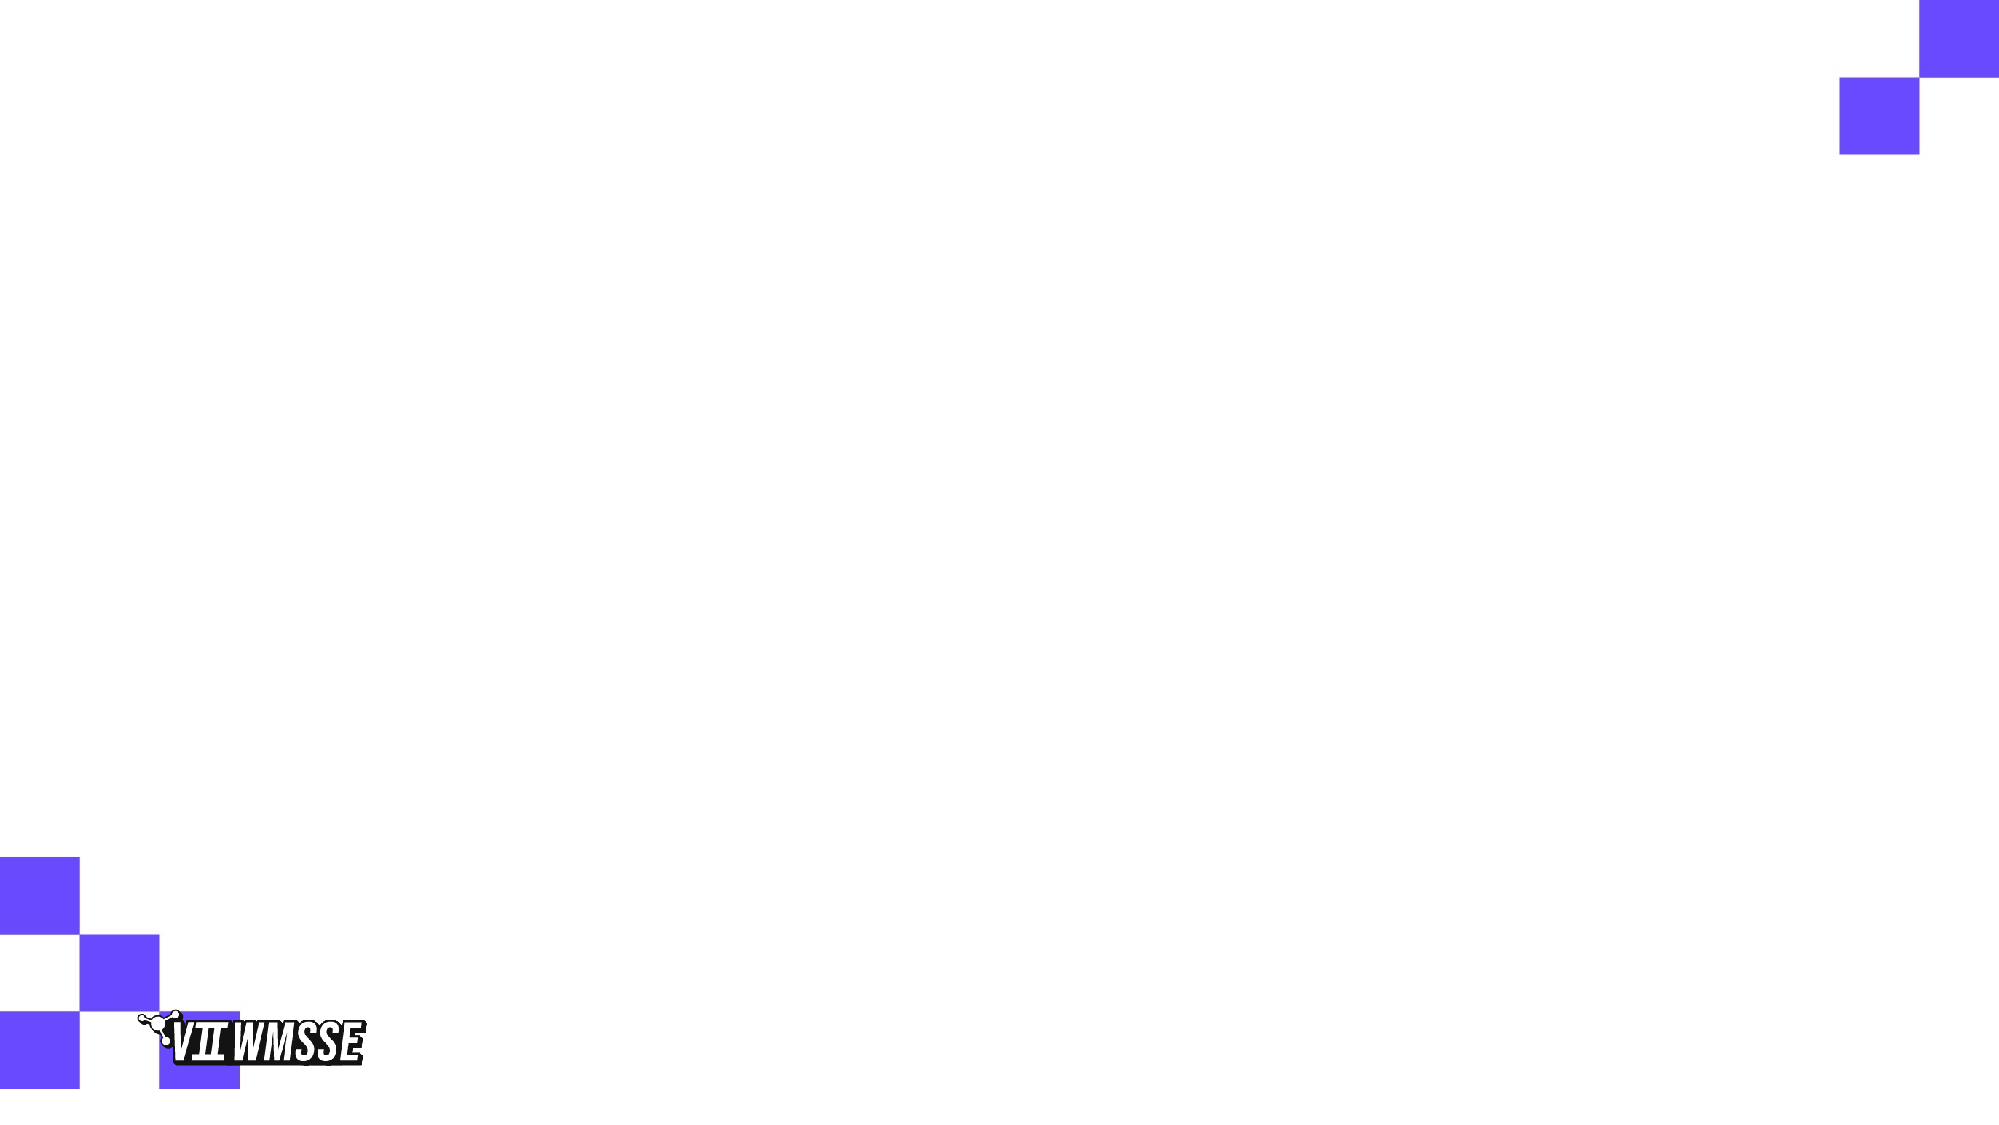
\includegraphics[width=\paperwidth,height=\paperheight]{Fondos/Cuerpo.pdf}}

  % Forzamos color negro
  \setbeamercolor{frametitle}{fg=white}
  \setbeamercolor{normal text}{fg=black}
  \setbeamercolor{structure}{fg=black}

  \begin{frame}{Implementación Computacional}
    \scriptsize

    \begin{columns}[c]

      %=================================================
      % COLUMNA IZQUIERDA
      %=================================================
      \begin{column}{0.45\textwidth}

        %------------- HARDWARE ----------------
        \begin{block}{\centering \scriptsize Paralelización}
          \centering
          \begin{tabular}{lc}
            \hline
            \textbf{Parámetro} & \textbf{Valor} \\
            \hline
            CPUs disponibles & $128$ \\
            $n_{\mathrm{jobs}}$ & $65$ \\
            \hline
          \end{tabular}
        \end{block}
        \centering\textit{Tabla: Recursos de cómputo empleados.}

        \vspace{0cm}

        %------------- TIEMPOS ----------------
        \begin{block}{\centering \scriptsize Resultado para $N=2$}
          \centering
          \begin{tabular}{lc}
            \hline
            \textbf{Parámetro} & \textbf{Valor} \\
            \hline
            Tiempo total & $15475.5~s$ \\
            Duración & $4h~17m~55s$ \\
            Casos exitosos & $26/26$ \\
            \hline
          \end{tabular}
        \end{block}
        \centering\textit{Tabla: Tiempos de ejecución.}

        \vspace{0.25cm}
        \centering
        Simulaciones resueltas mediante\\
        gTDGL usando \texttt{pyTDGL}

      \end{column}

      %=================================================
      % COLUMNA DERECHA
      %=================================================
      \begin{column}{0.5\textwidth}

        \begin{block}{\centering \scriptsize Magnitudes obtenidas}
          \vspace{0.1cm}
          \begin{itemize}
            \item Mapas de densidad de pares de Cooper
            \item Distribución espacial de corrientes
            \item Curvas $V-I$
            \item Extracción de corrientes críticas
            \item Cálculo de eficiencia del diodo:
          \end{itemize}
          \vspace{0.2cm}
          \centering
          \[
            \eta = \frac{\left|\, |J_c^+|-|J_c^-| \,\right|}{|J_c^+|+|J_c^-|} \times 100
          \]
          \vspace{0.1cm}
        \end{block}
        \centering\textit{Tabla: Magnitudes y métrica de eficiencia.}

      \end{column}

    \end{columns}
  \end{frame}
}





%========================9===========================

{
  \usebackgroundtemplate{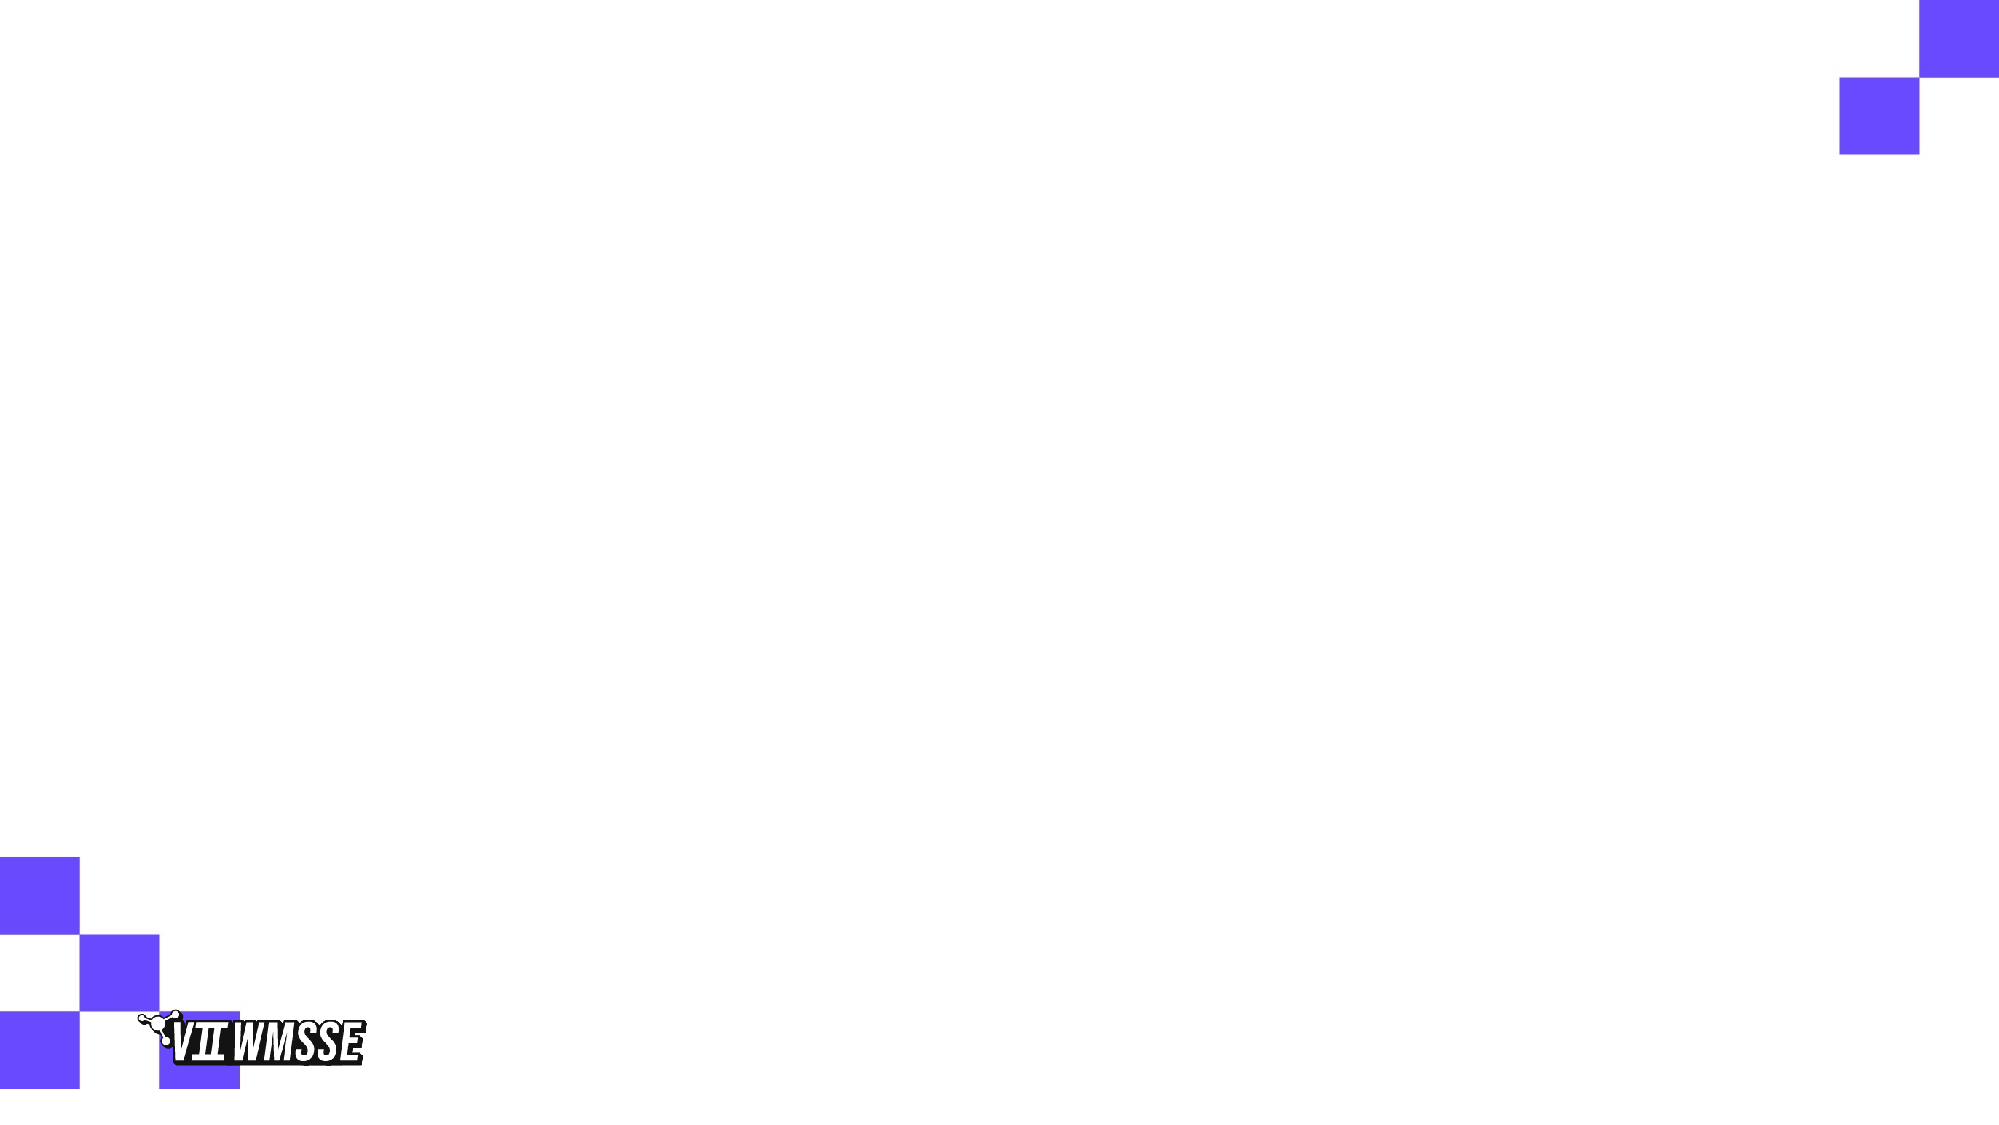
\includegraphics[width=\paperwidth,height=\paperheight]{Fondos/Cuerpo.pdf}}

  % Forzamos color negro
  \setbeamercolor{frametitle}{fg=white}
  \setbeamercolor{normal text}{fg=black}
  \setbeamercolor{structure}{fg=black}
  \setbeamercolor{itemize item}{fg=black}

\section{Resultados}
\begin{frame}{Resultados}
    \framesubtitle{Subtítulo aquí}
    
    \scriptsize
    \begin{columns}[t]
      
      % COLUMNA IZQUIERDA
      \begin{column}{0.48\textwidth}
        \begin{block}{\centering Densidad de Pares de Cooper}
          \centering
          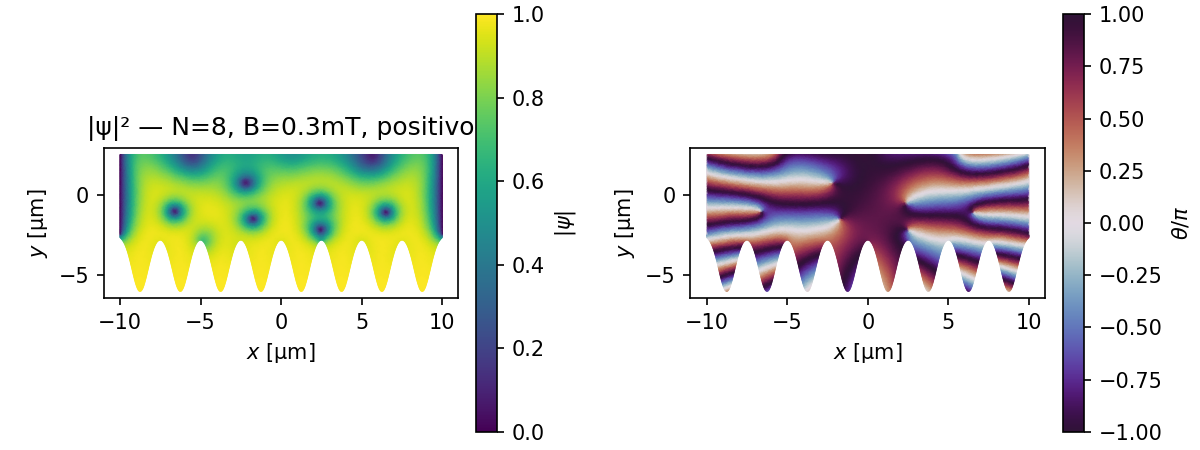
\includegraphics[width=\textwidth]{Imagenes/0.3_densidad_cooper.png}
        \end{block}
        \centering\textit{Figura: Representación densidad pares de Cooper.}
        
        \vspace{0.3cm}
        Aparición de vórtices de Abrikosov.
      \end{column}

      % COLUMNA DERECHA
      \begin{column}{0.48\textwidth}
        \begin{block}{\centering Mapa de corrientes}
          \centering
          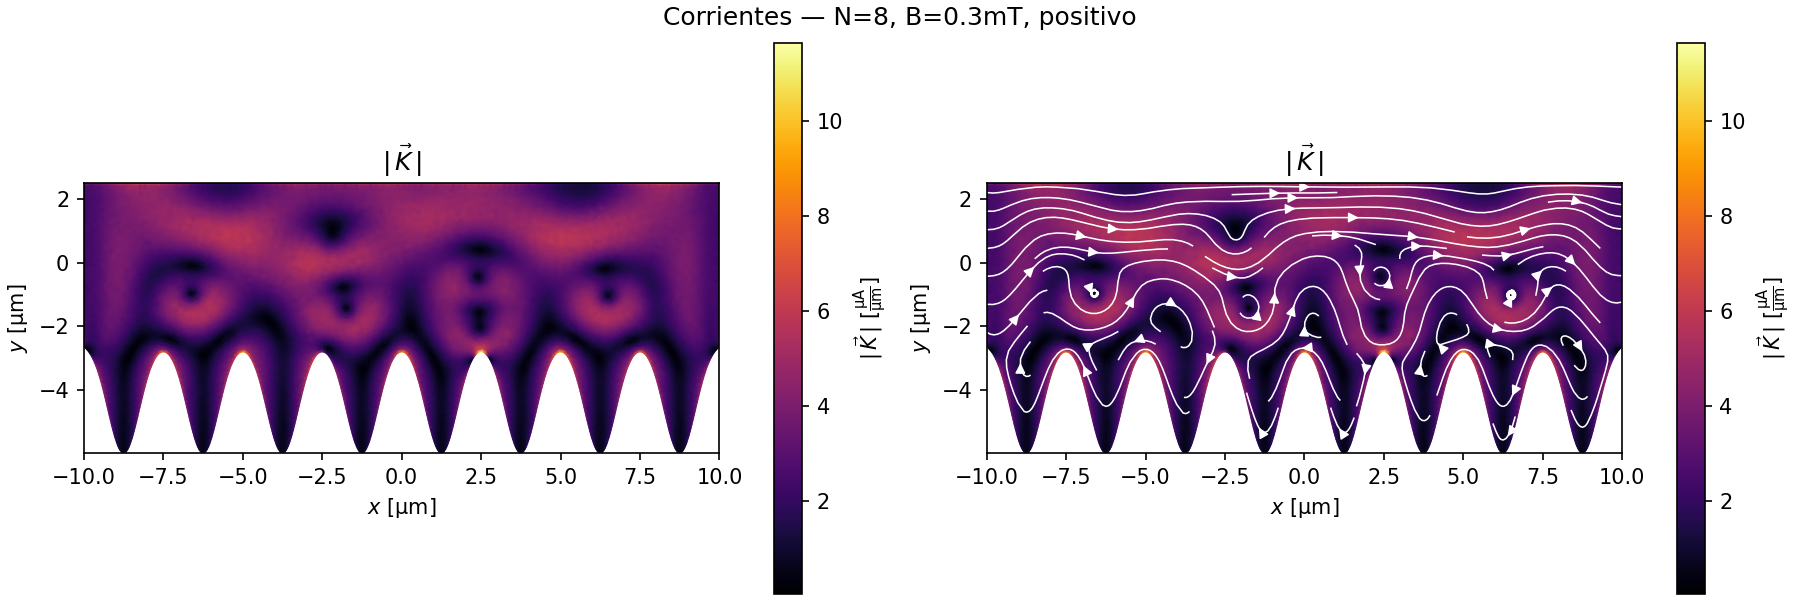
\includegraphics[width=\textwidth]{Imagenes/0.3_mapa_corrientes.png}
        \end{block}
        \centering\textit{Figura: Mapa de corrientes con visualizacion de vórtices.}
        
        \vspace{0.3cm}
        Se observa la dinámica de la corriente dentro del diodo.
      \end{column}

    \end{columns}
  \end{frame}
}

{
  \usebackgroundtemplate{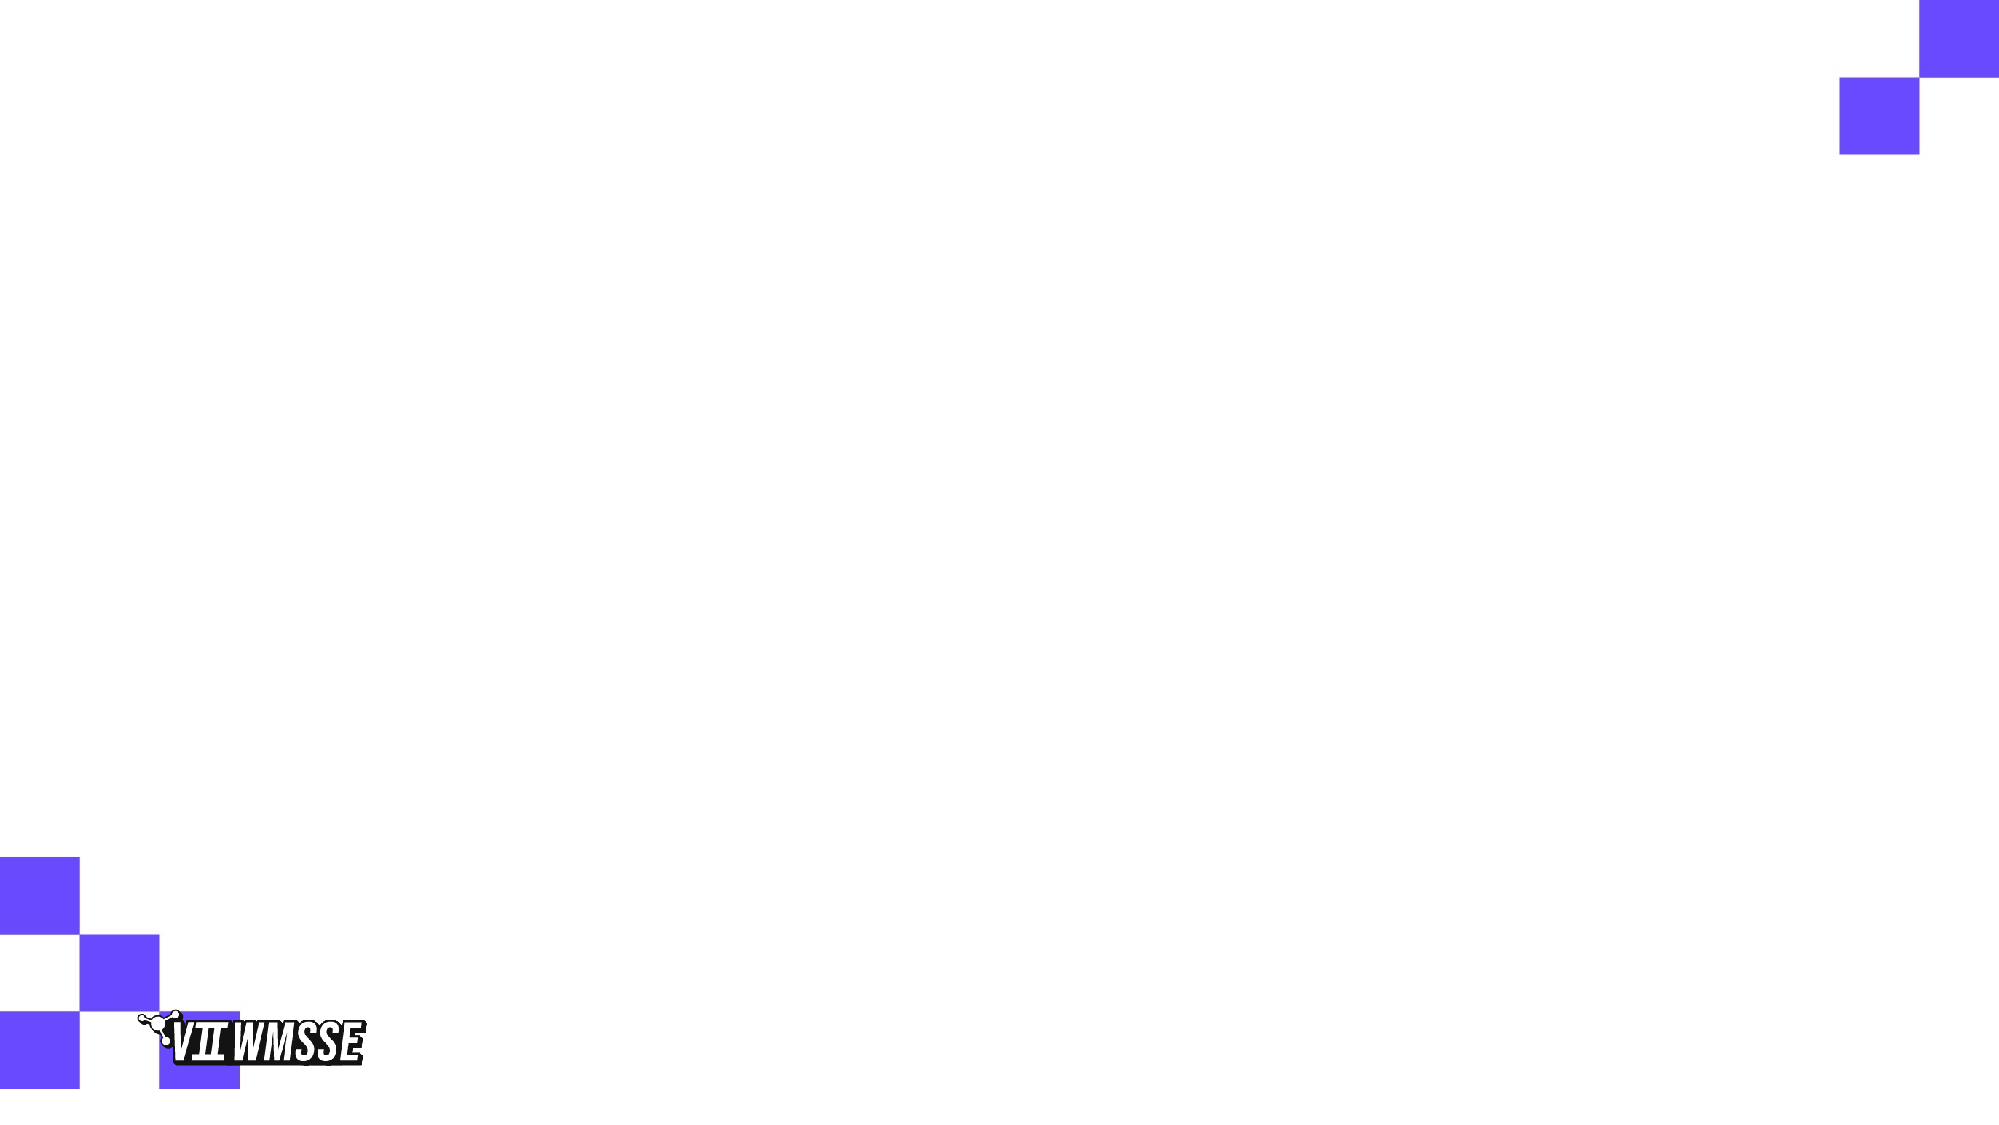
\includegraphics[width=\paperwidth,height=\paperheight]{Fondos/Cuerpo.pdf}}

  % Forzamos color negro
  \setbeamercolor{frametitle}{fg=white}
  \setbeamercolor{normal text}{fg=black}
  \setbeamercolor{structure}{fg=black}
  \setbeamercolor{itemize item}{fg=black}

\begin{frame}{Resultados}
    \framesubtitle{Subtítulo aquí}
    
    \scriptsize
    \begin{columns}[t]
      
      % COLUMNA IZQUIERDA
      \begin{column}{0.48\textwidth}
        \begin{block}{\centering Curva V vs I}
          \centering
          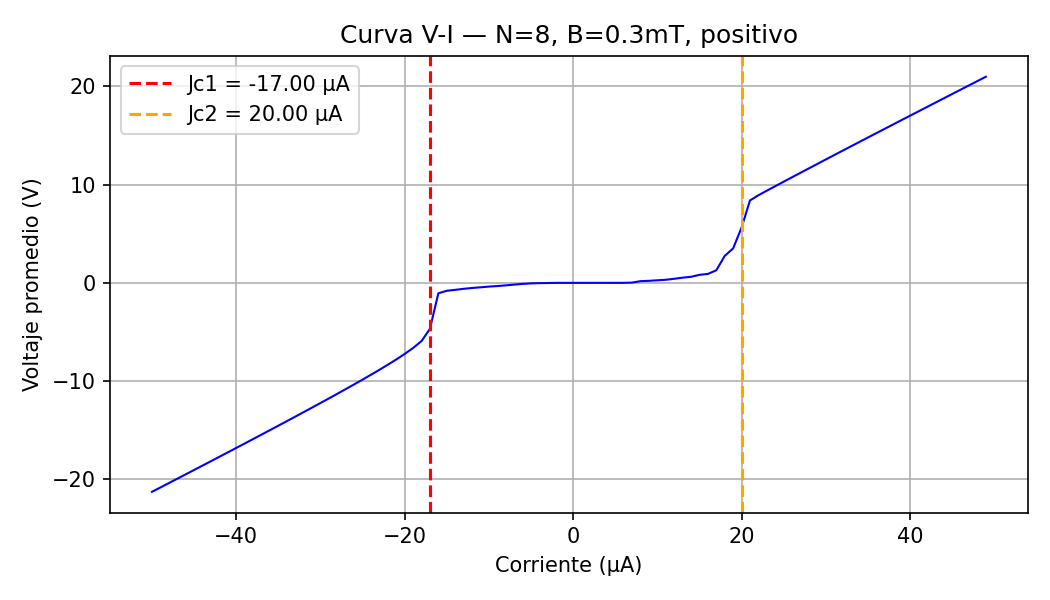
\includegraphics[width=\textwidth]{Imagenes/0.3_curva_VI.png}
        \end{block}
        \centering\textit{Figura: Corrientes con los saltos de Shapiro (asimetría).}

      \end{column}

      % COLUMNA DERECHA
      \begin{column}{0.48\textwidth}
        \begin{block}{\centering Eficiencia de 8 Crestas}
          \centering
          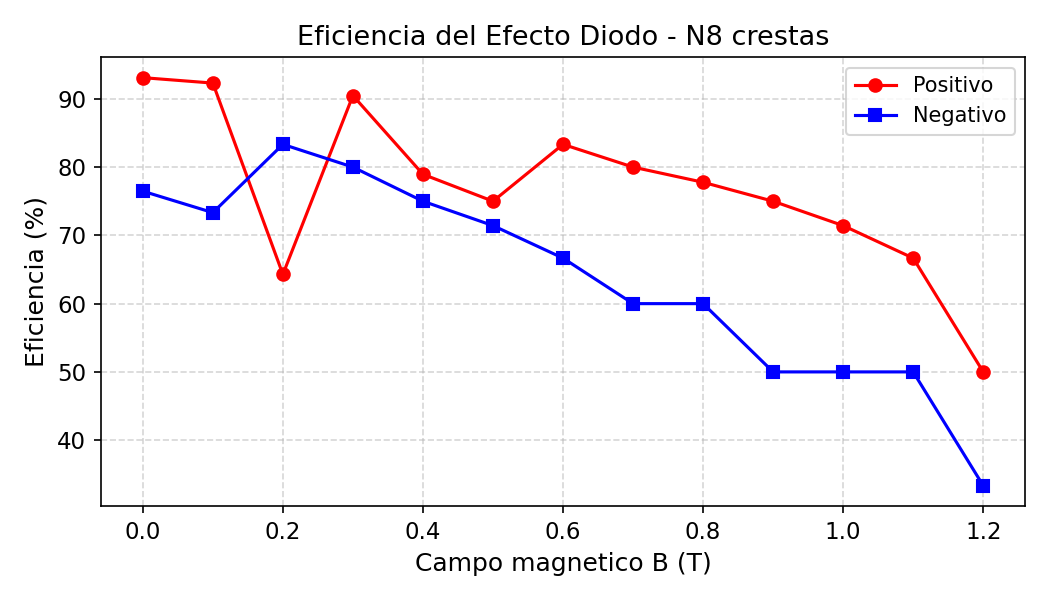
\includegraphics[width=\textwidth]{Imagenes/eficiencia_N8_crestas.png}
        \end{block}
        \centering\textit{Figura: Resultados de variaciones de campo magnético.}

      \end{column}

    \end{columns}
  \end{frame}
}


{
  \usebackgroundtemplate{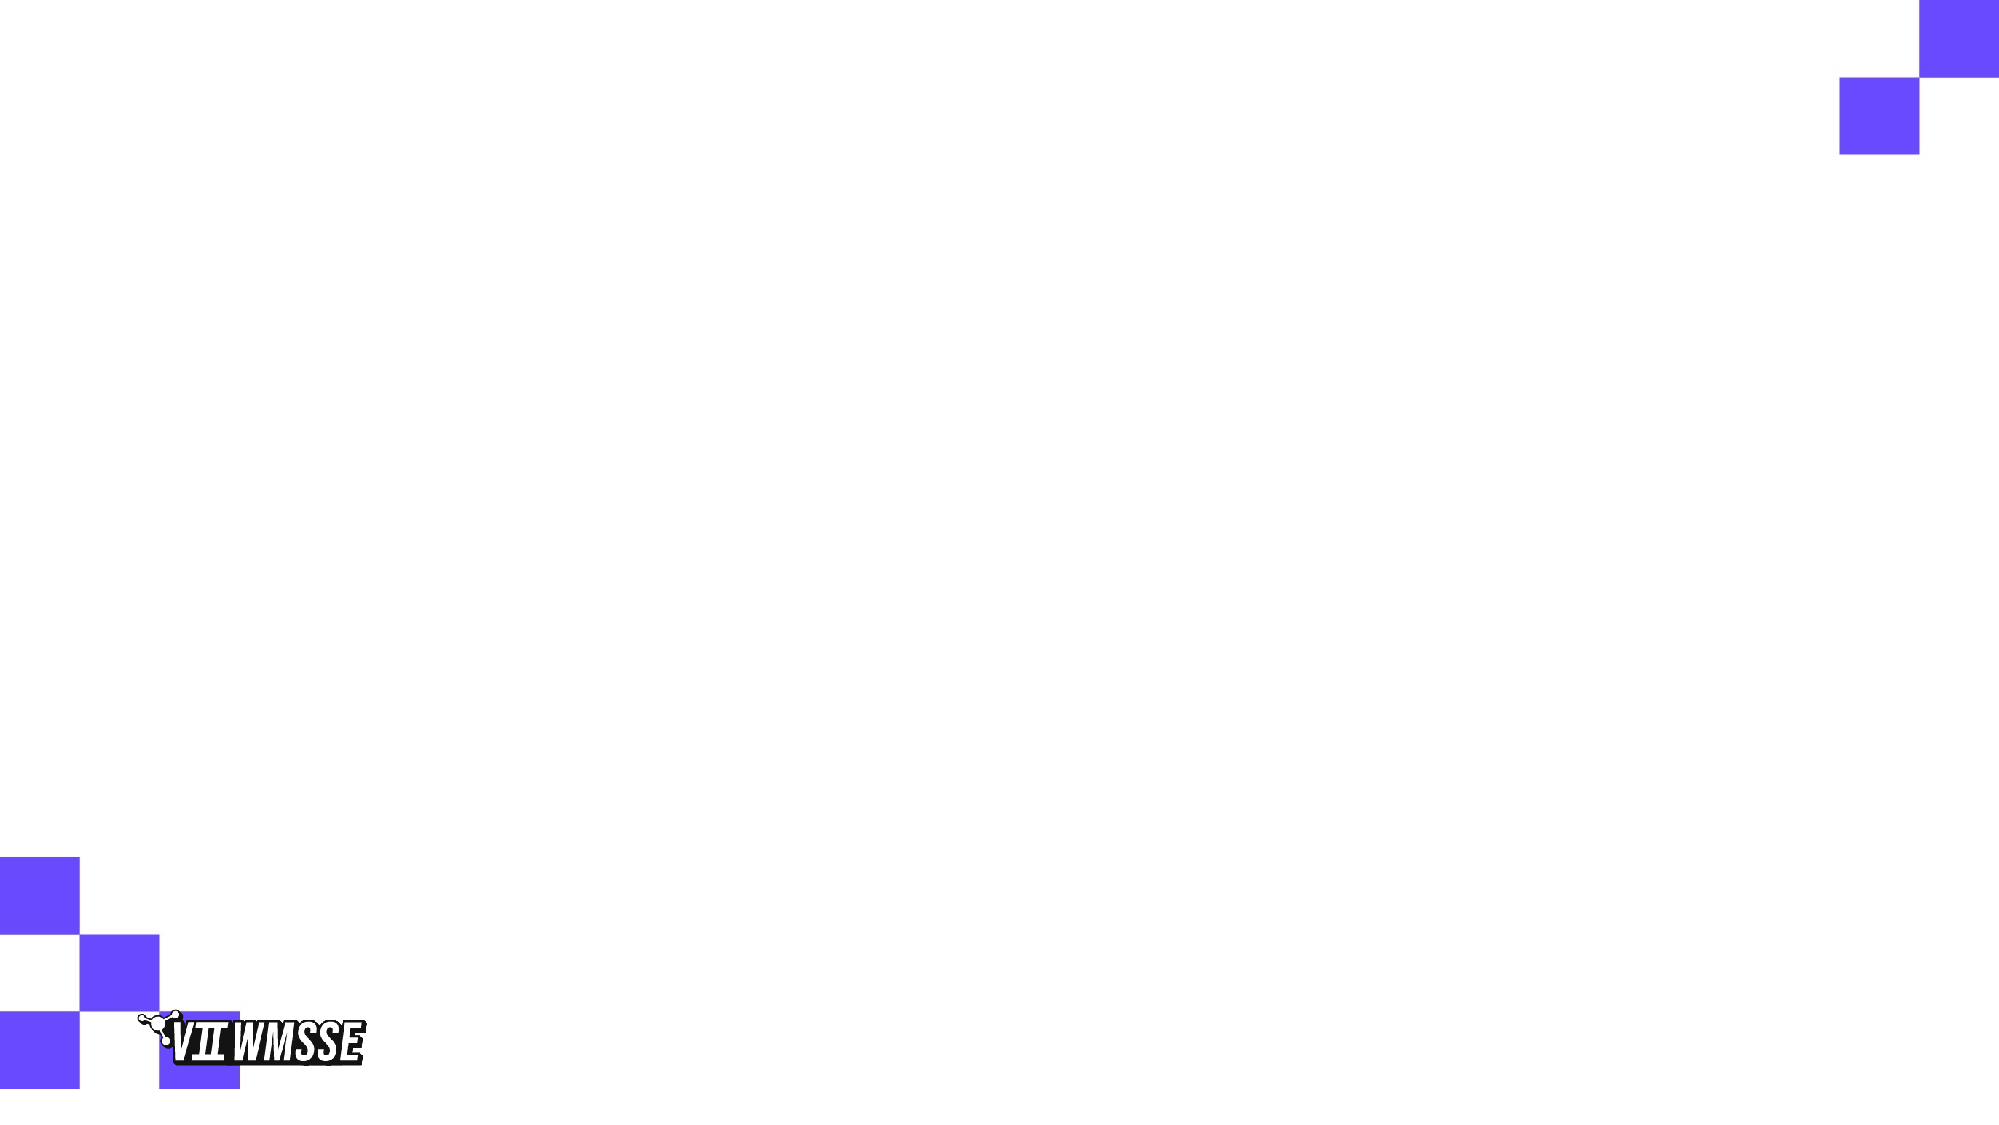
\includegraphics[width=\paperwidth,height=\paperheight]{Fondos/Cuerpo.pdf}}

  % Forzamos color negro
  \setbeamercolor{frametitle}{fg=white}
  \setbeamercolor{normal text}{fg=black}
  \setbeamercolor{structure}{fg=black}
  \setbeamercolor{itemize item}{fg=black}

\begin{frame}{Resultados}
    \framesubtitle{Subtítulo aquí}
    
    \scriptsize
        \vspace{-0.8cm}
    \begin{columns}[t]
      % COLUMNA IZQUIERDA
      \begin{column}{0.48\textwidth}
        \begin{block}{\centering Eficiencia Global}
          \centering
          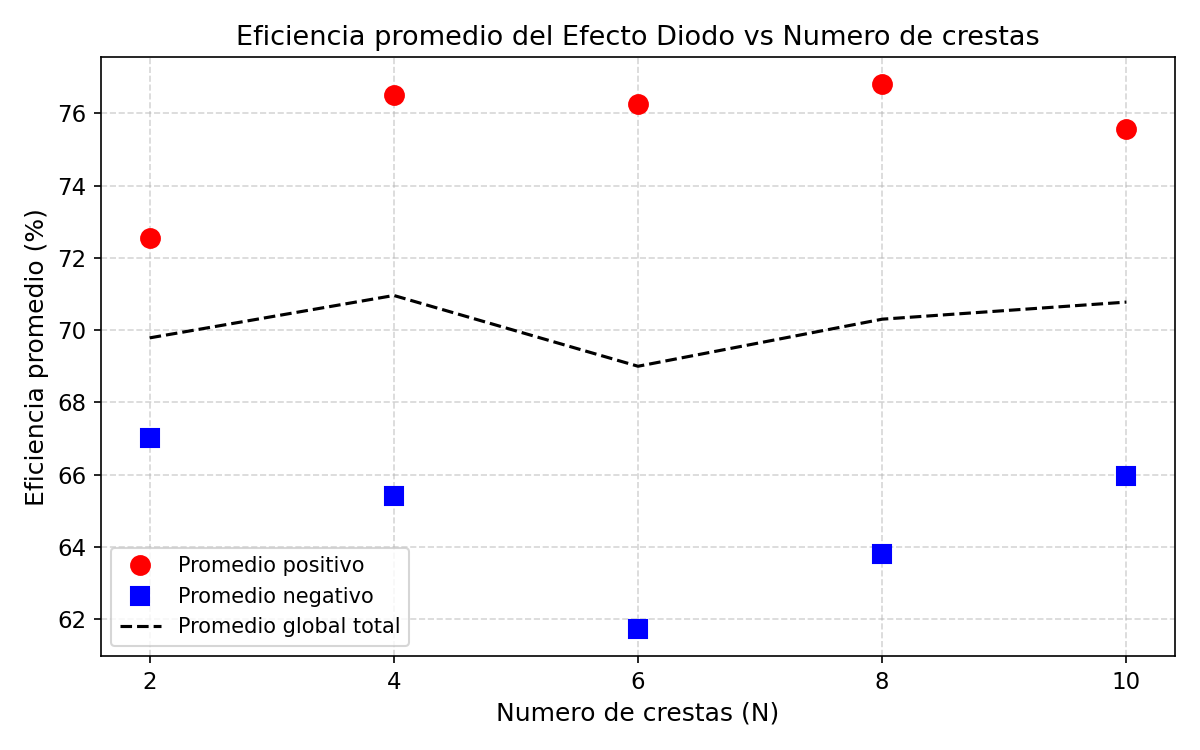
\includegraphics[width=\textwidth]{Imagenes/eficiencia_global.png}
        \end{block}
        \centering\textit{Figura: Rendimiento Global del Diodo.}
      
      \end{column}

      % COLUMNA DERECHA
    \begin{column}{0.48\textwidth}
  % Asegura el centrado de la columna
         \centering 
  
        \vspace{2.5cm}
  
  % Usamos una parbox para controlar el ancho y el centrado del texto
            \parbox{0.9\textwidth}{
                \centering
            Se ve el rendimiento general del Diodo, se puede ver los valores de eficiencia promedio a los que apuntan los resultados.
                    }
            \end{column}

    \end{columns}
  \end{frame}
}



%======================10=============================
{
\usebackgroundtemplate{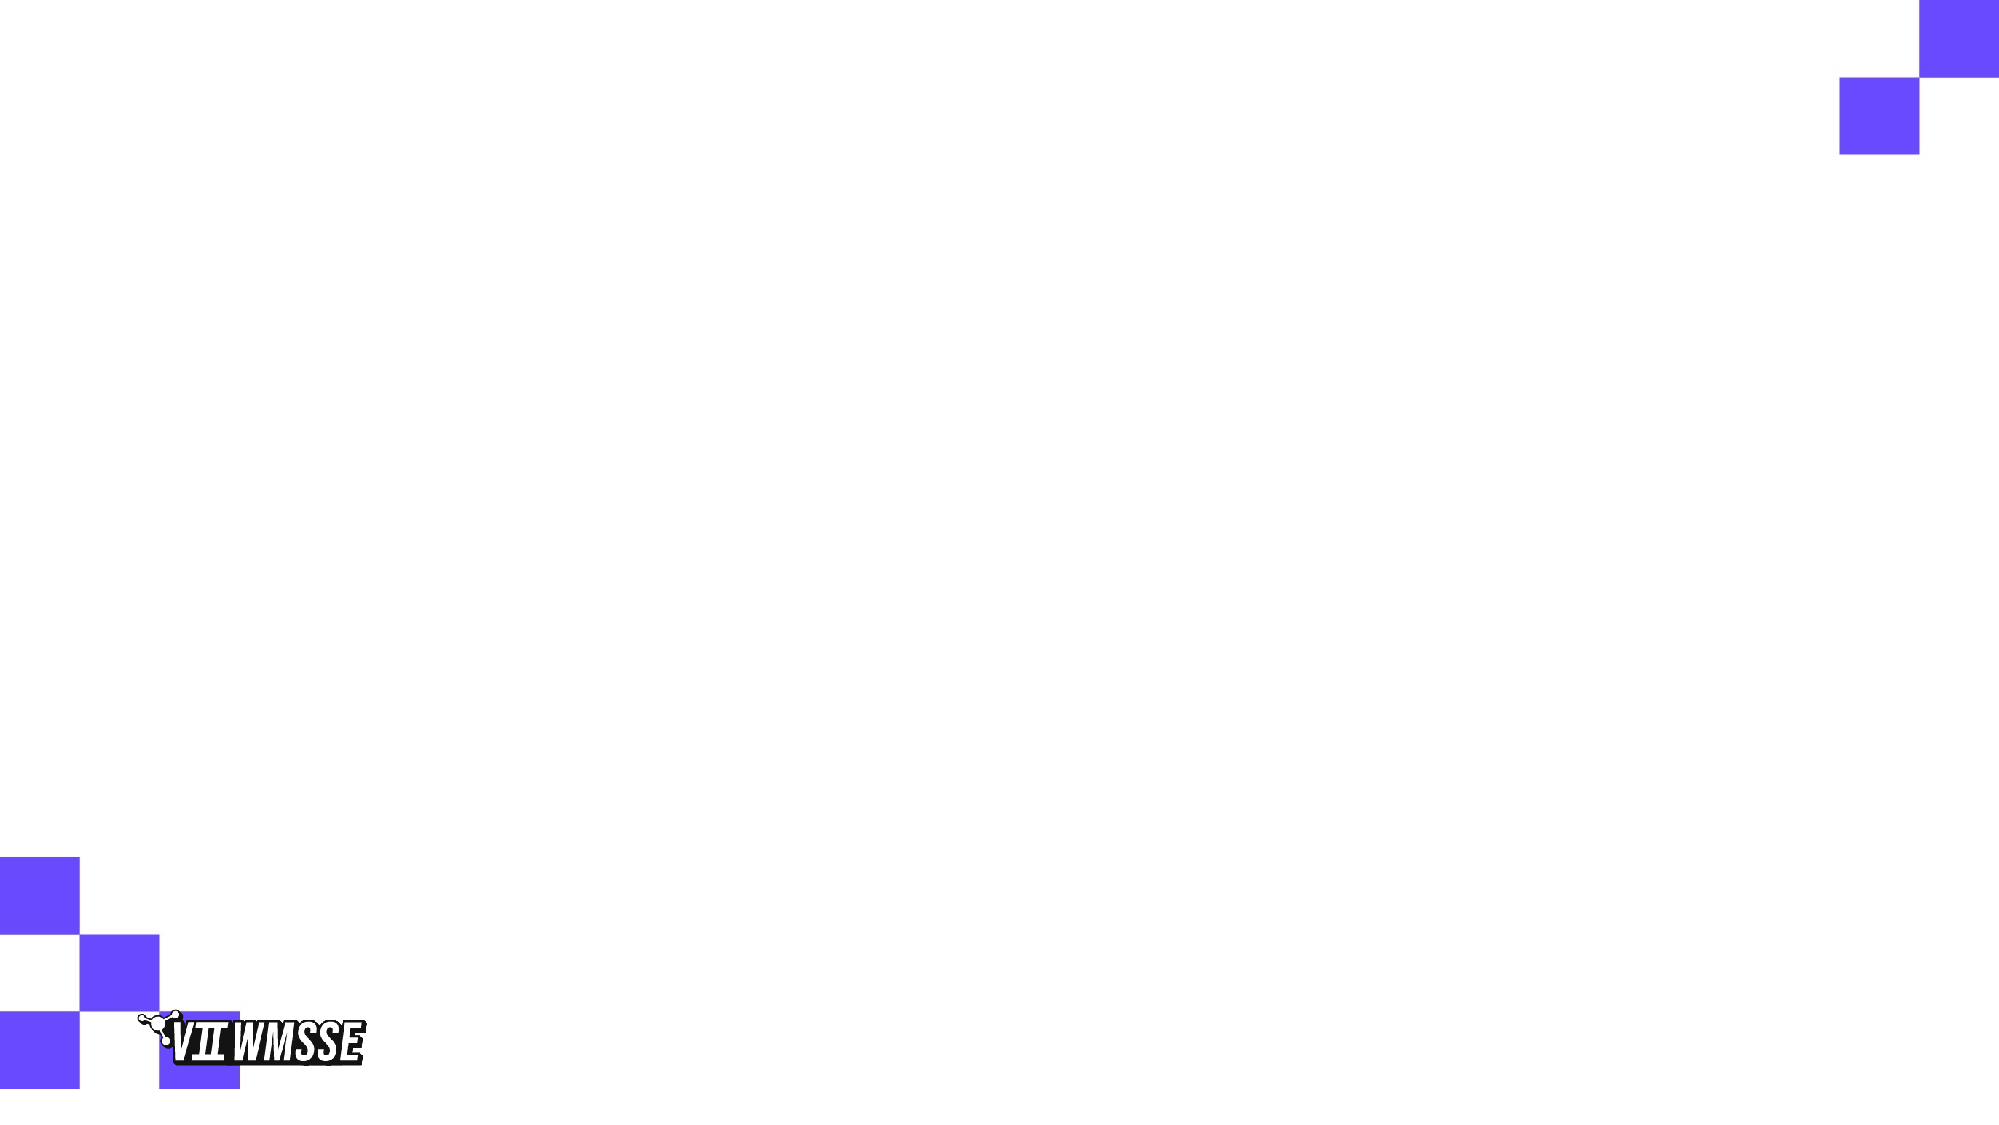
\includegraphics[width=\paperwidth,height=\paperheight]{Fondos/Cuerpo.pdf}}
\setbeamercolor{frametitle}{fg=white}
\setbeamercolor{normal text}{fg=black}
\setbeamercolor{structure}{fg=black}
\setbeamercolor{itemize item}{fg=black}
\section{Conclusiones}
\begin{frame}{Conclusiones}
\framesubtitle{Efecto Diodo Superconductor en geometría de crestas}

\begin{itemize}
    \item La eficiencia del efecto diodo alcanzó valores cercanos al \textbf{70\%}, confirmando una fuerte no-reciprocidad en la corriente crítica del sistema.

    \item La asimetría entre polaridades es directamente observable en los \textbf{saltos de la resistencia diferencial} $dV/dI$: los picos de $J_c^+$ y $J_c^-$ aparecen desplazados, evidenciando la ruptura de simetría inducida por la geometría de crestas.

    \item El efecto diodo se manifiesta en todas las configuraciones evaluadas ($N = 2, 4, 6, 8, 10$ crestas), con la eficiencia modulada por la densidad de crestas y el campo magnético aplicado.

    \item Bajo polaridad negativa, las crestas actúan como trampas direccionales de vórtices, retardando la disipación y elevando $|J_c^-|$ respecto a $|J_c^+|$.
\end{itemize}

\end{frame}
}



% ==========================================================
% FIN: Letras Blancas
% ==========================================================
{
  \usebackgroundtemplate{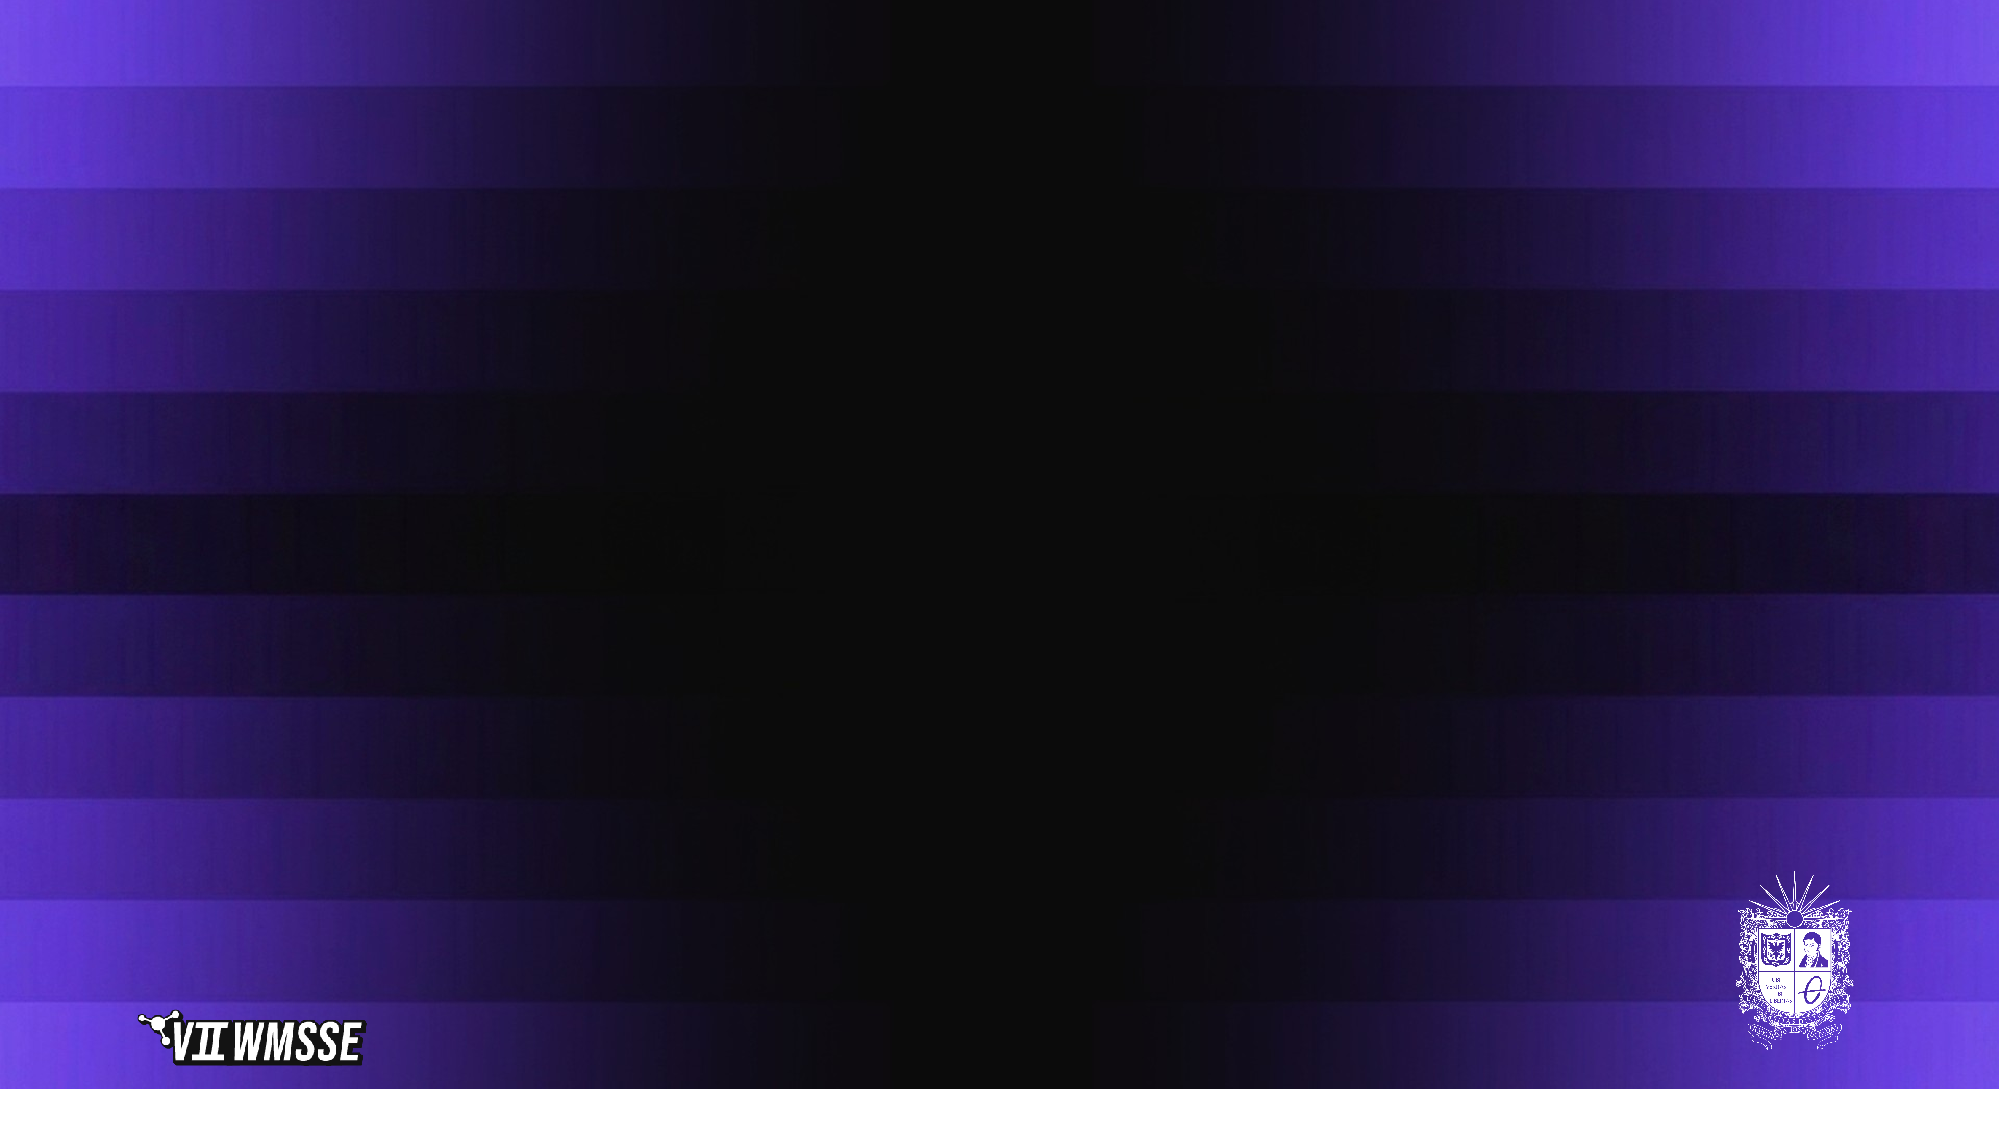
\includegraphics[width=\paperwidth,height=\paperheight]{Fondos/fin.pdf}}
  
  % Forzamos color blanco
  \setbeamercolor{frametitle}{fg=white}
  \setbeamercolor{normal text}{fg=white}
  \setbeamercolor{structure}{fg=white}

  \begin{frame}
      \centering
      \vspace{2cm}
      {\Huge \textcolor{white}{\textbf{¡Muchas gracias por su atención!}}}
      
      \vspace{1cm}
      {\large \textcolor{white}{¿Alguna pregunta?}}
  \end{frame}
}

\end{document}